\part{概率论与数理统计}

\chapter{概率论的基本概念}%============================15

\begin{flushright}
    \begin{tabular}{r|||}
        \textit{“概率论,当局限在适当的范围内,应该同样引起数学家、实验者和政治家的兴趣。”}\\
        ——\textit{德·摩根}
    \end{tabular}
\end{flushright}

概率论是数学的一个分支,研究随机事件的发生概率和随机现象的规律性. 它是研究不确定性的一种工具和方法. 

概率论的基本概念包括随机试验、样本空间、事件、概率等. 随机试验是指具有多种可能结果的试验,例如掷硬币、抛骰子等. 样本空间是指随机试验的所有可能结果的集合. 事件是样本空间的子集,表示试验中我们感兴趣的一些结果. 概率是事件发生的可能性的度量,通常用一个介于 0 和 1 之间的数来表示. 

概率论的基本原理包括古典概型、几何概型和统计概型. 古典概型适用于试验结果的数量有限且每个结果发生的可能性相等的情况,例如抛硬币、掷骰子等. 几何概型适用于试验结果的数量无限且每个结果发生的可能性相等的情况,例如在一条直线上选择一个点的位置. 统计概型适用于试验结果的数量无限且每个结果发生的可能性不相等的情况,例如从一副牌中抽取一张牌. 

概率论的应用广泛,包括统计学、金融学、物理学、工程学、生物学等领域. 它可以用于描述随机现象的规律性、进行风险评估和决策分析、进行数据分析和建模等. 概率论提供了一种量化不确定性的方法,帮助我们理解和解决各种实际问题. 
\section{随机事件及其概率}

\subsection{事件的运算}

\begin{theorem}[交换律]
    $\sj{A} \cup \sj{B}=\sj{B} \cup \sj{A},~\sj{A} \sj{B}=\sj{B} \sj{A} .$
\end{theorem}

\begin{theorem}[结合律]
    $\sj{A} \cup \sj{B} \cup \sj{C}=(\sj{A} \cup \sj{B}) \cup \sj{C}=\sj{A} \cup(\sj{B} \cup \sj{C}),~\sj{A} \sj{B} \sj{C}=(\sj{A} \sj{B}) \sj{C}=\sj{A}(\sj{B} \sj{C}) .$\\
    特别地 $(\sj{A} \cup \sj{B}) \cap \sj{C}=\sj{A} \cup(\sj{B} \cap \sj{C})$ 不一定成立,比如当 $ \sj{A} \neq \varnothing,~\sj{B}=\Omega,~\sj{C}=\varnothing $ 时,该式不成立.
\end{theorem}

\begin{theorem}[和与积的分配律]
    $(\sj{A} \cup \sj{B}) \cap \sj{C}=(\sj{A} \cap \sj{C}) \cup(\sj{B} \cap \sj{C}),~(\sj{A} \cap \sj{B}) \cup \sj{C}=(\sj{A} \cup \sj{C}) \cap(\sj{B} \cup \sj{C}) .$
\end{theorem}

\begin{theorem}[差与积的分配律]
    $(\sj{A}-\sj{B}) \cap \sj{C}=(\sj{A} \cap \sj{C})-(\sj{B} \cap \sj{C}),~(\sj{A} \cap \sj{B})-\sj{C}=(\sj{A}-\sj{C}) \cap(\sj{B}-\sj{C}) .$
\end{theorem}

\begin{theorem}[和与差的分配律]
    $(\sj{A} \cup \sj{B})-\sj{C}=(\sj{A}-\sj{C}) \cup(\sj{B}-\sj{C})$\\
    特别地 $(\sj{A}-\sj{B}) \cup \sj{C}=(\sj{A} \cup \sj{C})-(\sj{B} \cup \sj{C})$ 不一定成立,比如当 $ \sj{A}=\sj{B},~\sj{C} \neq \varnothing $ 时,该式不成立.
\end{theorem}

\begin{theorem}[对偶律]
    $\overline{\sj{A} \cup \sj{B}}=\bar{\sj{A}} \bar{\sj{B}},~\overline{\sj{A} \sj{B}}=\bar{\sj{A}} \cup \bar{\sj{B}},~\overline{\sj{A} \cup \sj{B} \cup \sj{C}}=\bar{\sj{A}} \bar{\sj{B}} \bar{\sj{C}},~\overline{\sj{A} \sj{B} \sj{C}}=\bar{\sj{A}} \cup \bar{\sj{B}} \cup \bar{\sj{C}} .$
\end{theorem}

\begin{theorem}[和差转换]
    \begin{enumerate}[label=(\arabic{*})]
        \item 差: $\sj{A}-\sj{B}=\begin{cases}
                      \sj{A}-\sj{A} \sj{B}=\sj{A} \bar{\sj{B}} \\ \sj{A}-\sj{B} \sj{A}=\bar{\sj{B}} \sj{A}.
                  \end{cases}$
        \item 和: $\sj{A} \cup \sj{B}=\begin{cases}
                      (\sj{A}-\sj{B}) \cup \sj{B}=\sj{A} \bar{\sj{B}} \cup \sj{B}=\bar{\sj{B}} \sj{A} \cup \sj{B} \\ \sj{A} \cup(\sj{B}-\sj{A})=\sj{A} \cup \bar{\sj{A}} \sj{B}=\sj{A} \cup \sj{B} \bar{\sj{A}}.
                  \end{cases}$
    \end{enumerate}
\end{theorem}

\subsection{概率的性质}

\begin{theorem}
    $P(\varnothing)=0,~ P(\Omega)=1 .$
\end{theorem}

\begin{theorem}[有限可加性]
    设 $ \sj{A}_{1},~\sj{A}_{2},~\cdots,~\sj{A}_{n} $ 是两两互不相容的事件,则有
    $$P\left(\sj{A}_{1} \cup \sj{A}_{2} \cup \cdots \cup \sj{A}_{n}\right)=P\left(\sj{A}_{1}\right)+P\left(\sj{A}_{2}\right)+\cdots+P\left(\sj{A}_{n}\right)$$
    \begin{enumerate}[label=(\arabic{*})]
        \item 事件 $\sj{S}$ 被分成两个不相容的事件 $\sj{S}_{1},~\sj{S}_{2}\left(\sj{S}_{1} \sj{S}_{2}=\varnothing,~\sj{S}_{1} \cup \sj{S}_{2}=\sj{S}\right)$,
        则 $ P(\sj{S})=P\left(\sj{S}_{1}\right)+P\left(\sj{S}_{2}\right)$;
        \item 若 $ \sj{S}_{1} \subset \sj{S}$,则 $ P\left(\sj{S}-\sj{S}_{1}\right)=P(\sj{S})-P\left(\sj{S}_{1}\right).$
    \end{enumerate}
\end{theorem}

\begin{theorem}[求逆公式]
    $P\qty(\bar{\sj{A}})=1-P(\sj{A}).$
\end{theorem}

\begin{example}
    设 $\sj{A},\sj{B}$ 为两个随机事件,若 $P(\sj{AB})=0.25,~P(\sj{B})=0.3,~P(\sj{A}\cup\sj{B})=0.6$,求 $P\qty(\sj{A}\mid\overline{\sj{B}})$.
\end{example}
\begin{solution}
    如图 \ref{figures/ven1.pdf} 所示,则 $P\qty(\sj{A}\mid\overline{\sj{B}})=\dfrac{P\qty(\sj{A\overline{B}})}{P\qty(\overline{\sj{B}})}=\dfrac{0.3}{1-P(\sj{B})}=\dfrac{3}{7}.$
\end{solution}

\begin{minipage}[b]{0.3\linewidth}
    \begin{figure}[H]
        \centering
        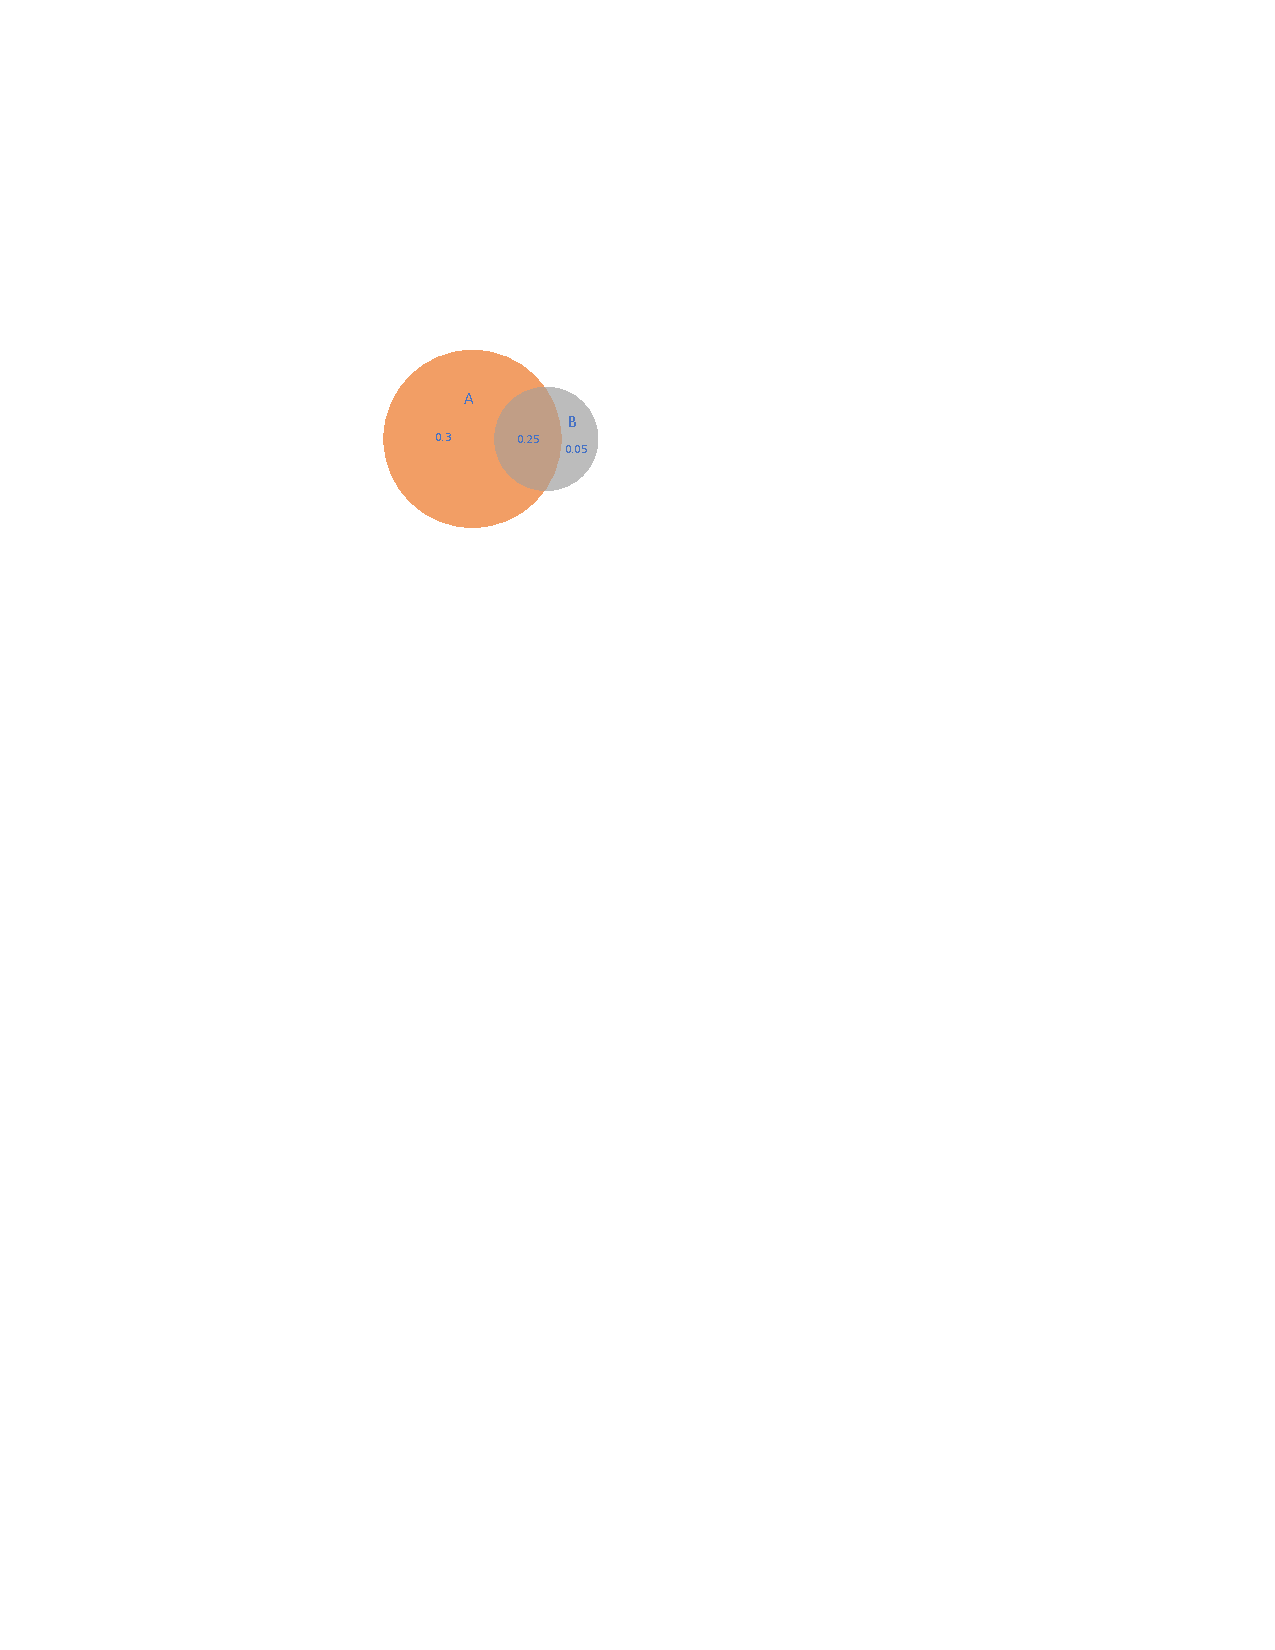
\includegraphics[scale=0.8]{figures/ven1.pdf}
        \caption{}
        \label{figures/ven1.pdf}
    \end{figure}
\end{minipage}\hfill
\begin{minipage}[b]{0.3\linewidth}
    \begin{figure}[H]
        \centering
        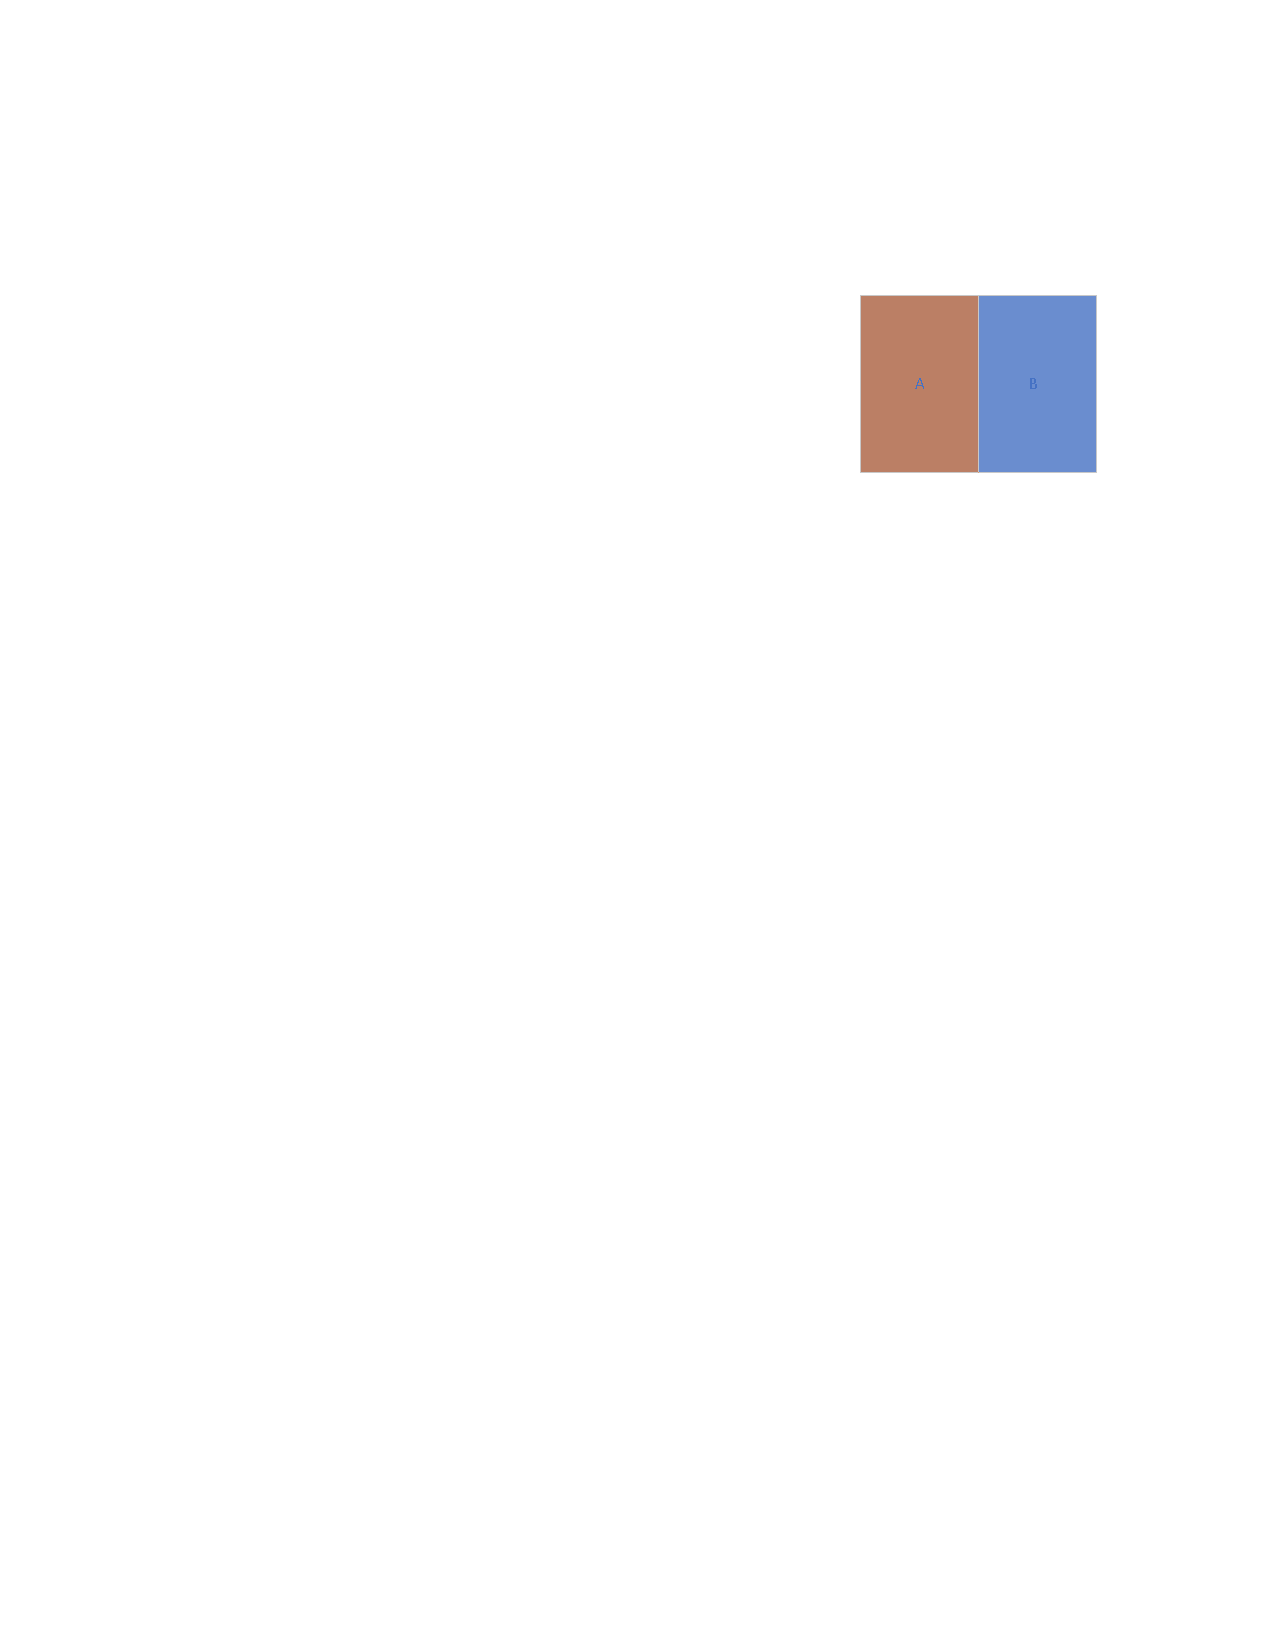
\includegraphics[scale=0.8]{figures/ven2.pdf}
        \caption{}
        \label{figures/ven2.pdf}
    \end{figure}
\end{minipage}\hfill
\begin{minipage}[b]{0.3\linewidth}
    \begin{figure}[H]
        \centering
        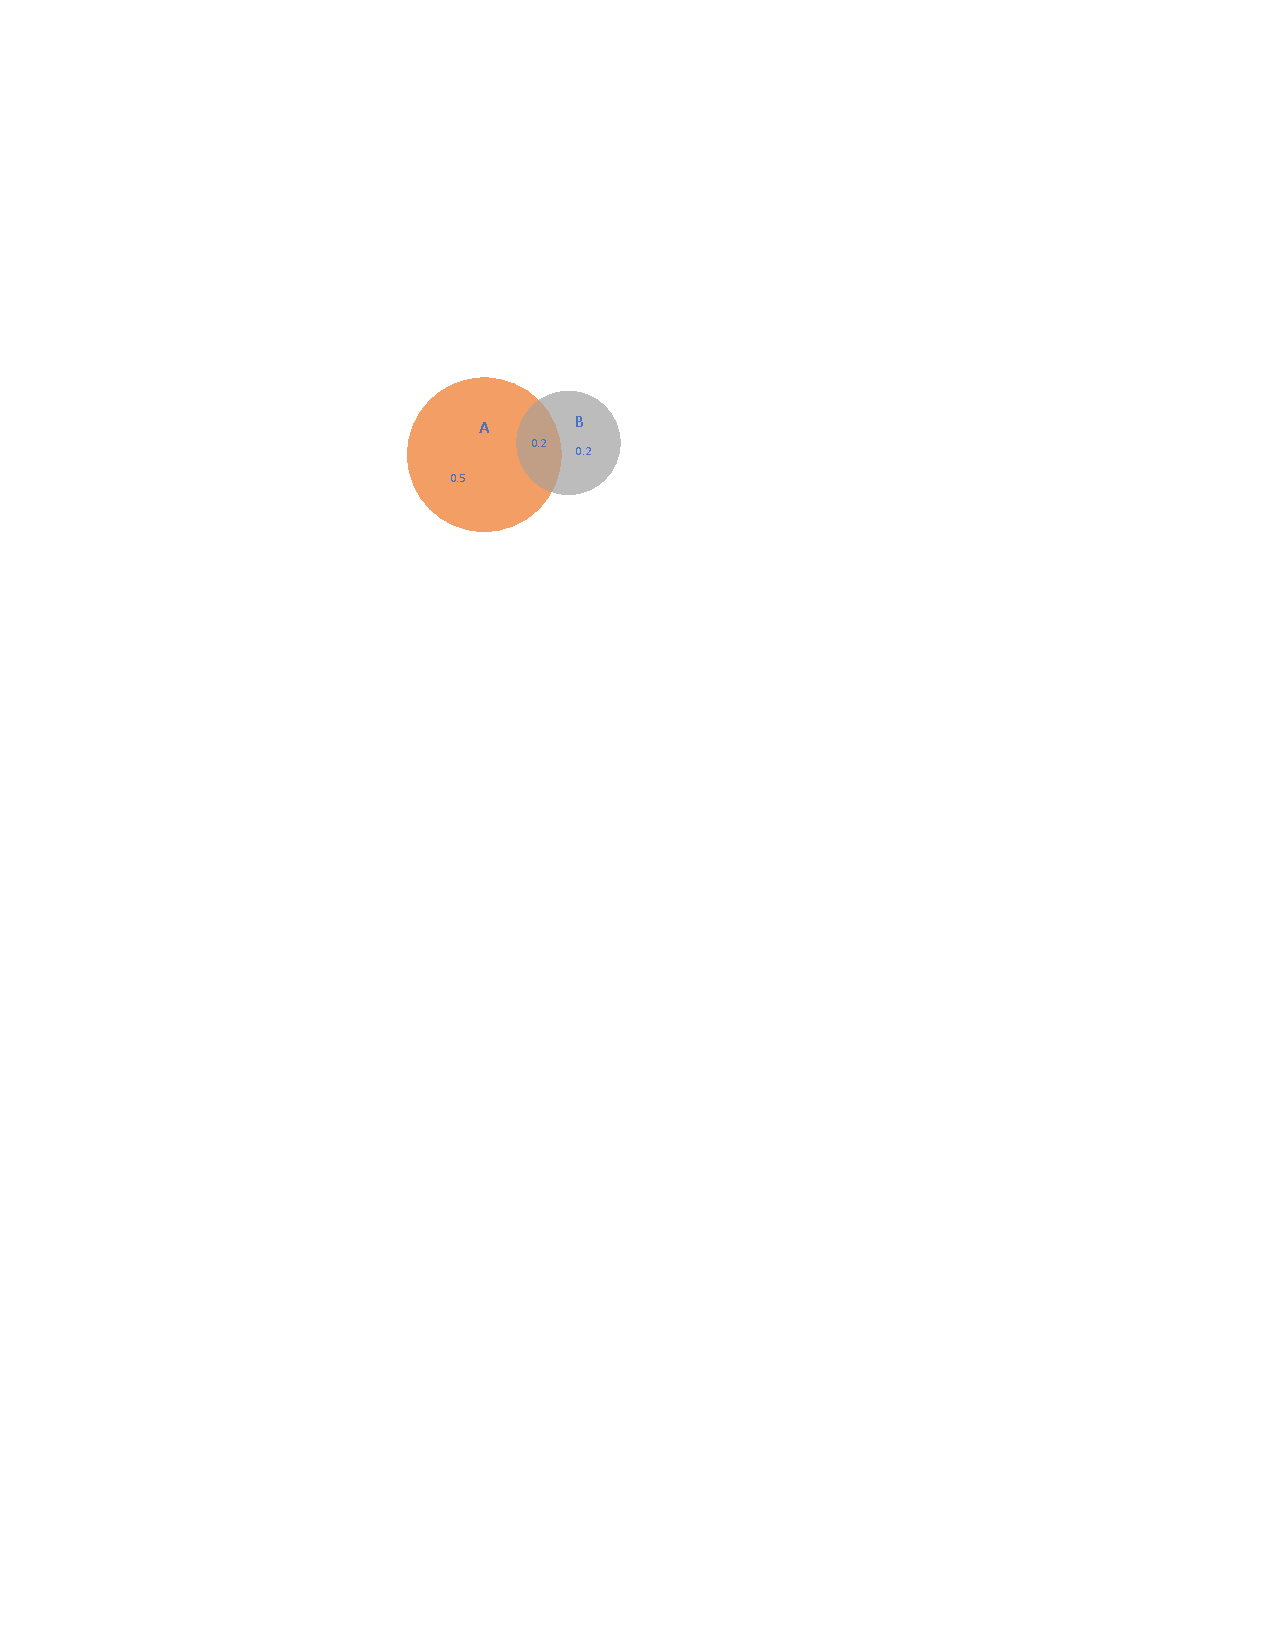
\includegraphics[scale=0.8]{figures/ven3.pdf}
        \caption{}
        \label{figures/ven3.pdf}
    \end{figure}
\end{minipage}

\begin{example}
    设 $\sj{A},\sj{B}$ 为随机事件,$\sj{AB}=\overline{\sj{A}}~\overline{\sj{B}},~0<P(\sj{B})<1$,求 $P\qty(\sj{A}\mid\overline{\sj{B}})+P\qty(\overline{\sj{A}}\mid\sj{B}).$
\end{example}
\begin{solution}
    因为 $\sj{AB}=\overline{\sj{A}}~\overline{\sj{B}}$,所以事件 $\sj{A}+\sj{B}=\Omega$,如图 \ref{figures/ven2.pdf} 所示,
    则 $P\qty(\sj{A}\mid\overline{\sj{B}})+P\qty(\overline{\sj{A}}\mid\sj{B})=P(\sj{A}\mid\sj{A})+P(\sj{B}\mid\sj{B})=1+1=2.$
\end{solution}

\begin{example}
    已知 $P\qty(\overline{\sj{A}})=0.3,~P(\sj{B})=0.4,~P(\sj{A}-\sj{B})=0.5$,求 $P\qty{\sj{B}\mid \qty(\sj{A}\cup\overline{\sj{B}})}.$
\end{example}
\begin{solution}
    由题意可作出如图 \ref{figures/ven3.pdf} 所示的 ven 图,则 $P\qty{\sj{B}\mid \qty(\sj{A}\cup\overline{\sj{B}})}=\dfrac{P\qty(\sj{B}\cap\qty(\sj{A}\cup\overline{\sj{B}}))}{P\qty(\sj{A}\cup\overline{\sj{B}})}=\dfrac{P(\sj{AB})}{1-P(\sj{AB})}=0.25.$
\end{solution}

% 子性质三:  
% 子性质四:  P(\sj{A} \bar{\sj{B}})=P(\sj{A})-P(\sj{A} \sj{B})  (减法公式)
% 性质三 (减法公式):  P(\sj{A}-\sj{B})=P(\sj{A} \bar{\sj{B}})=P(\sj{A})-P(\sj{A} \sj{B}) 
% 若  \sj{B} \subset \sj{A},~P(\sj{A}-\sj{B})=P(\sj{A})-P(\sj{B}) 
% 若  \sj{A} \sj{B}=\varnothing,~P(\sj{A}-\sj{B})=P(\sj{A}) 
% 性质四 (加法公式):  P(\sj{A} \cup \sj{B})=P(\sj{A})+P(\sj{B})-P(\sj{A} \sj{B}) 
%  P(\sj{A} \cup \sj{B} \cup C)=P(\sj{A})+P(\sj{B})+P(C)-P(\sj{A} \sj{B})-P(\sj{A} C)-P(\sj{B} C)+P(\sj{A} \sj{B} C) 
% 证明:  P(\sj{A} \sj{B})+P(\sj{A} C)+P(\sj{B} C)+1 \geqslant P(\sj{A})+P(\sj{B})+P(C) 
% 性质五:  P(\sj{A} \sj{B})=P(\sj{A}) \Leftrightarrow P(\sj{A} \cup \sj{B})=P(\sj{B}) \Leftrightarrow P(\sj{A}-\sj{B})=0 
% 性质六:  P(\sj{A} \sj{B})=0 \Leftrightarrow P(\sj{A} \bar{\sj{B}})=P(\sj{A}) \Leftrightarrow P(\sj{B} \bar{\sj{A}})=P(\sj{B}) 
% 有关不等式的性质
% 性质七:  0 \leqslant P(\sj{A}) \leqslant 1 
% 性质入: 若  \sj{S} \subset T ,~则  P(\sj{S}) \leqslant P(T) 
% 子性质一:  P(\sj{A} \sj{B}) \leqslant P(\sj{A}),~P(\sj{B}) \leqslant P(\sj{A} \cup \sj{B}),~P(\sj{A} \sj{B}) \leqslant \frac{P(\sj{A})+P(\sj{B})}{2} \leqslant P(\sj{A} \cup \sj{B}) 
% 子性质二:
% 
% \begin{array}{l}
% P(\sj{A})=0 \Rightarrow\left\{\begin{array}{l}
% P(\sj{A} \sj{B})=0 \\
% P(\sj{A} \cup \sj{B})=P(\sj{B})
% \end{array}\right. \\
% P(\sj{A})=1 \Rightarrow\left\{\begin{array}{l}
% P(\sj{A} \cup \sj{B})=1 \\
% P(\sj{A} \sj{B})=P(\sj{B})
% \end{array}\right. \\
% P(\sj{A} \sj{B})=1 \Rightarrow P(\sj{A})=P(\sj{B})=1
% \end{array}


\subsection{古典概率与几何概率}

\subsubsection{古典概率}

\begin{example}
    求 10 个不同规格的零件中混入 3 个次品,现进行逐个检查,则查完 5 个零件时正好查出 3 个次品的概率.
\end{example}
\begin{solution}
    \textbf{法一: }记 $\mathsf{A}=\text{查完 5 个零件正好查出 3 个次品}$,那么事件 $\mathsf{A}$ 由两个事件构造: $$\mathsf{B}=\text{前 4 次检查,查出 2 个次品},\mathsf{C}=\text{第 5 次检查,查出的是次品}$$
    即 $\mathsf{A}=\mathsf{BC}$,由乘法公式 $P(\mathsf{A})=P(\mathsf{BC})=P(\mathsf{B})P(\mathsf{C}|\mathsf{B})$,前 4 次检查中有 2 个正品和 2 个次品的组合为
    $$P(\mathsf{B})=\dfrac{\C_3^2\cdot\C_7^2}{\C_{10}^4}=\dfrac{3}{10}$$
    已知 $\mathsf{B}$ 发生的条件下,剩下 6 个零件中查出 1 个次品的概率为 $\dfrac{1}{6}$,即 $P(\mathsf{C}|\mathsf{B})=\dfrac{1}{6}$,于是 $P(\mathsf{A})=\dfrac{3}{10}\times\dfrac{1}{6}=\dfrac{1}{20}.$\\
    \textbf{法二: }事件 $\sj{A}$ 等价于在 3 个次品中选一个放在第 5 个位置上,然后在 7 个正品中选 2 个与余下的 2 个次品排在前 4 个位置上,最后将其余 5 个正品随意排在后面 5 个位置上,所以
    $$P(\sj{A})=\dfrac{\C_3^1\C_7^2\C_2^2\cdot 4!\cdot5!}{10!}=\dfrac{1}{20}.$$
    \textbf{法三: }考虑 3 只次品在 10 次检查中的位置,问题转化为前 4 个位置中选 2 个放次品,第 5 个位置必须放次品,于是 $$P(\sj{A})=\dfrac{\C_4^2\cdot1}{\C_{10}^3}=\dfrac{1}{20}.$$
    \textbf{法四:}只考虑放正品的位置,则前 4 个位置需要放 2 个正品,后 5 个位置全为正品,则 $P(\sj{A})=\dfrac{\C_4^2\C_5^5}{\C_{10}^3}=\dfrac{1}{20}$
\end{solution}

\subsubsection{几何概率}

\subsection{概率基本公式及条件概率}

\begin{theorem}[与独立有关的条件概率]
    设 $P(\sj{B})\in(0,1)$,则 $\sj{A} $ 与 $\sj{B}$ 相互独立的充要条件为:
    \begin{enumerate}[label=(\arabic{*})]
        \item $P(\sj{A}\mid\sj{B})=P\qty(\sj{A}\mid \bar{\sj{B}})$;
        \item $P(\sj{A}\mid\sj{B})+P\qty(\bar{\sj{A}}\mid \bar{\sj{B}})=1$;
        \item $P\qty(\bar{\sj{A}}\mid \sj{B})+P\qty(\sj{A}\mid \bar{\sj{B}})=1$.
    \end{enumerate}
\end{theorem}

\subsection{全概率公式和 Bayes 公式}

\begin{definition}[完备事件组]
    设 $ \sj{B}_{1}, \sj{B}_{2}, \cdots, \sj{B}_{n} $ 为试验 $ E $ 的一组事件,$\Omega $ 为样本空间,若满足以下两个条件:
    \begin{enumerate}[label=(\arabic{*})]
        \item $\sj{B}_{i} \sj{B}_{j}=\emptyset, i \neq j, i, j=1,2, \cdots, n $;
        \item $\sj{B}_{1} \cup \sj{B}_{2} \cup \cdots \cup \sj{B}_{n}=\Omega $.
    \end{enumerate}
    则称 $ \sj{B}_{1}, \sj{B}_{2} \cdots, \sj{B}_{n} $ 是一个完备事件组,也称 $ \sj{B}_{1}, \sj{B}_{2}, \cdots, \sj{B}_{n} $ 为样本空间 $ \Omega $ 的一个划分.
\end{definition}

\begin{theorem}[全概率公式与 Bayes 公式]
    设 $ \Omega $ 为试验 $ E $ 的样本空间,$\sj{B}_{1}, \sj{B}_{2}, \cdots, \sj{B}_{n} $ 为 $ \Omega $ 的一个划分,且 $ P\left(\sj{B}_{i}\right)>0~~(i=1,2, \cdots, n) $,则
    \begin{flalign*}
    P(\sj{A})=\sum_{i=1}^{n} P\left(\sj{B}_{i}\right) P\left(\sj{A} \mid \sj{B}_{i}\right) 
    =P\left(\sj{A} \mid \sj{B}_{1}\right) P\left(\sj{B}_{1}\right)+P\left(\sj{A} \mid \sj{B}_{2}\right) P\left(\sj{B}_{2}\right)+ 
    \cdots+P\left(\sj{A} \mid \sj{B}_{n}\right) P\left(\sj{B}_{n}\right)
    \end{flalign*}
    称为全概率公式. 而
    $$P\left(\sj{B}_{i} \mid \sj{A}\right)=\frac{P\left(\sj{B}_{i} \sj{A}\right)}{P(\sj{A})}=\frac{P\left(\sj{A} \mid \sj{B}_{i}\right) P\left(\sj{B}_{i}\right)}{\displaystyle\sum_{j=1}^{n} P\left(\sj{A} \mid \sj{B}_{j}\right) P\left(\sj{B}_{j}\right)}~~(i=1,2, \cdots, n)  $$
    称为 Bayes 公式.
\end{theorem}

\begin{example}
    一条生产线生产 $n$ 件产品不出故障的概率为 $\dfrac{\lambda^n}{n!}\e^{-\lambda}~~(n=0,1,\cdots)$ 若每件产品合格的概率为 $p~~(0<p<1)$,且各产品是否合格相互独立,
    求该生产线在两次故障之间共生产 $k~~(k=0,1,\cdots)$ 件合格品的概率.
\end{example}
\begin{solution}
    设事件 $\sj{A}_i=$“两次故障之间生产的产品总个数为 $i~~(i=0,1,\cdots)$”,事件 $\sj{B}_k=$“两次故障之间生产的合格品个数为 ”$k~~(k=0,1,\cdots,i)$,那么事件 $\sj{B}_k$ 的概率为
    \begin{flalign*}
        P\qty{\sj{B}_k} & =\sum_{i=0}^{\infty}P\qty{\sj{A}_i}\cdot P\qty{\sj{B}_k\mid \sj{A}_i}=\sum_{i=k}^{\infty}P\qty{\sj{A}_i}\cdot P\qty{\sj{B}_k\mid \sj{A}_i}=\sum_{i=k}^{\infty}\qty(\dfrac{\lambda^i}{i!}\e^{-\lambda})\cdot\qty[\C_i^kp^k(1-p)^{i-k}]                           \\
                        & =\e^{-\lambda}p^k\sum_{i=k}^{\infty}\dfrac{\lambda^i}{i!}\C_i^k(1-p)^{i-k}=\e^{-\lambda}p^k\sum_{i=0}^{\infty}\dfrac{\lambda^{i+k}}{(i+k)!}\C_{i+k}^k(1-p)^{i}=\e^{-\lambda}p^k\lambda^k\sum_{i=0}^{\infty}\dfrac{\lambda^i}{(i+k)!}\dfrac{(i+k)!}{k!i!}(1-p)^i \\
                        & =\dfrac{1}{k!}\e^{-\lambda}p^k\lambda^k\sum_{i=0}^{\infty}\dfrac{\qty[\lambda(1-p)]^i}{i!}=\dfrac{1}{k!}\e^{-\lambda}p^k\lambda^k\cdot\eval{\e^x}_{x=\lambda(1-p)}=\e^{-\lambda p}\dfrac{(p\lambda)^k}{k!}
    \end{flalign*}
\end{solution}
\section{事件的独立性}


\chapter{随机变量及其分布}%============================16

\begin{flushright}
    \begin{tabular}{r|||}
        \textit{“我创建了形貌随机征象的一种概率散布.。”}\\
        ——\textit{泊松}
    \end{tabular}
\end{flushright}

随机变量是一个可以随机取不同值的变量, 其取值是由随机事件的结果决定的. 随机变量可以是离散的, 也可以是连续的. 

随机变量的分布描述了其取不同值的概率分布情况. 常见的随机变量分布包括: 
\begin{enumerate}
    \item 离散型随机变量的分布: \begin{enumerate}
        \item 二项分布: 描述了在一次伯努利试验中成功的次数的分布. 
        \item 泊松分布: 描述了在一段时间内某事件发生次数的分布. 
        \item 几何分布: 描述了在一系列独立伯努利试验中首次成功所需的次数的分布. 
    \end{enumerate}
    \item 连续型随机变量的分布: \begin{enumerate}
        \item 正态分布: 也称为高斯分布, 是最常见的连续型随机变量分布, 具有钟形曲线. 
        \item 均匀分布: 描述了在一个区间内各个数值出现的概率相同的分布. 
        \item 指数分布: 描述了连续时间内某事件发生的间隔时间的分布. 
    \end{enumerate}
\end{enumerate}

除了以上列举的分布外, 还有众多其他类型的随机变量分布, 每种分布都有其特定的数学形式和特征. 在统计学和概率论中, 随机变量及其分布是研究的重要对象, 用来描述和分析随机现象的规律. 

\section{离散型随机变量的概率分布}

\subsection{离散型随机变量的分布函数}

\begin{definition}[分布函数]
    设离散型随机变量 $ X $ 的分布律为
    $P\left\{X=x_{k}\right\}=p_{k},~k=1,2, \cdots,$ 则 $ X $ 的分布函数为
    $$F(x)=P\{X \leqslant x\}=\sum_{x_{k} \leqslant x} p_{k}$$
    或者
    $F(x)=\begin{cases}
            0,           & x<x_{1}                 \\
            p_{1},       & x_{1} \leqslant x<x_{2} \\
            p_{1}+p_{2}, & x_{2} \leqslant x<x_{3} \\
            \vdots       & \vdots
        \end{cases}$
\end{definition}

\begin{theorem}[分布函数的性质]
    以下三条是判定一个函数是否为分布函数的充要条件.
    \begin{enumerate}[label=(\arabic{*})]
        \item 单调性: $F(x) $ 是 $ x $ 的单调不减函数,即对于任意实数 $ x_{1}<x_{2}$,有 $ F\left(x_{1}\right) \leqslant F\left(x_{2}\right) $;
        \item 有界性: $\displaystyle0 \leqslant F(x) \leqslant 1 ,~F(-\infty)=\lim _{x \rightarrow-\infty} F(x)=0,~F(+\infty)=\lim_{x\to+\infty}F(x)=1$;
        \item 右连续: $F(x)$ 是 $x$ 的右连续函数,即对任意实数 $x$,有 $F(x^+)=F(x).$
    \end{enumerate}
\end{theorem}

\subsection{二项分布}

\begin{definition}[二项分布]
    在 $ n $ 重伯努利试验中,若用随机变量 $ X $ 表示所关心事件 $ \sj{A} $ 发生的次数,$P(\sj{A})=p~~(0<p<1)$,则 $ X $ 的分布律为
    $$P\{X=k\}=\C_{n}^{k} p^{k}(1-p)^{n-k}, ~k=0,1, \cdots, n$$
    则称 $ X $ 服从参数为 $ n, p $ 的二项分布,记作 $ X \sim B(n, p) $.
    \begin{enumerate}[label=(\arabic{*})]
        \item 0-1 分布可以视为 $ n=1 $ 时的二项分布;
        \item 若 $ X \sim B(n, p) $,令 $ Y=n-X$,则 $ Y \sim B(n, 1-p) .$
    \end{enumerate}
\end{definition}

% \subsection{离散型随机变量的性质}
% 
% \begin{example}
%     设随机变量 $X$ 的概率分布 $P\qty{X=k}=\dfrac{a}{k(k+1)},k=1,2,\cdots,$,其中 $a$ 为常数,$X$ 的分布函数为 $F(x)$,已知 $F(b)=\dfrac{3}{4}$,求 $b$ 的取值范围.
% \end{example}
% \begin{solution}
%     $\displaystyle \sum_{k=1}^{+\infty}P\qty{X=k}=\sum_{k=1}^{+\infty}\dfrac{a}{k(k+1)}=a\sum_{k=1}^{+\infty}\qty(\dfrac{1}{k}-\dfrac{1}{k+1})=a\lim_{k\to\infty}\qty(1-\dfrac{1}{k+1})=1\Rightarrow a=1$
%     则,$$F(x)=\sum_{k\leqslant x}\qty(\dfrac{1}{k}-\dfrac{1}{k+1})$$
%     当 $i\leqslant x<i+1$ 时,$$F(x)=\sum_{k\leqslant i}\qty(\dfrac{1}{k}-\dfrac{1}{k+1})=1-\dfrac{1}{i+1}$$
%     则 $F(b)=\dfrac{3}{4}=1-\dfrac{1}{4}\Rightarrow 3\leqslant b<4.$
% \end{solution}
% 
% \subsection{五大离散型分布}
\section{连续型随机变量的概率分布}

\subsection{连续型随机变量概率密度}

\begin{definition}[连续型随机变量概率密度]
    设随机变量 $ X $ 的分布函数是 $ F(x) $, 若存在一个非负可积函数 $ f(x) $, 使对于任意实数 $ x $, 都有
    $$F(x)=\int_{-\infty}^{x} f(t) \dd t ~(x \in \mathbb{R})$$
    则称 $ X $ 为连续型随机变量, 称 $ f(x) $ 为 $ X $ 的概率密度函数, 简称概率密度, 记为 $ X \sim f(x) .$
\end{definition}

\begin{theorem}[连续型随机变量概率密度的性质]
    概率密度 $ f(x) $ 的性质如下:
    \begin{enumerate}[label=(\arabic{*})]
        \item 非负性: $ f(x) \geqslant 0 $;
        \item 规范性: $ \displaystyle\int_{-\infty}^{+\infty} f(x) \mathrm{d} x=1$ ;
        \item 对任意实数 $ a \leqslant b$ 都有 $\displaystyle P\{a<X \leqslant b\}=\int_{a}^{b} f(x) \mathrm{d} x $;
        \item 若 $ f(x) $ 在点 $ x $ 处连续, 则有 $ F^{\prime}(x)=f(x) .$
    \end{enumerate}
\end{theorem}

设 $ X $ 是连续型随机变量, 已知其概率密度 $ f_{X}(x) $, 则由函数 $ y=g(x) $ 确定的随机变量 $ Y $ 可能是离散型随机变量, 也可能是连续型随机变量. \\
以连续为例, 求随机变量 $ Y $ 的分布函数 $ F_{Y}(y) $.
\begin{enumerate}[label=(\arabic{*})]
    \item 定义法: $\displaystyle F_{Y}(y)=P\{Y \leqslant y\}  =P\{g(X) \leqslant y\}  =\int_{g(x) \leqslant y} f_{X}(x) \mathrm{d} x$, 做题步骤:
          \begin{enumerate}
              \item 画出 $ y=g(x) $ 在 $ f(x) $ 正概率区间的图像;
              \item 找出 $ y=g(x) $ 在 $ y=y $ (动直线) 以下的图像, 确定该部分 $ x $ 的范围, 并用 $ y $ 表示;
              \item 求出 $ F_{Y}(y) $.
          \end{enumerate}
          若求连续型随机变量 $ Y $ 的概率密度 $ f_{Y}(y) $, 则分布函数 $ F_{Y}(y) $ 对 $ y $ 求导即可.
          $$
              f_Y(y)=\begin{cases}
                  \dfrac{\mathrm{d} F_{Y}(y)}{\mathrm{d} y}, & \text { 当 } F_{Y}(y) \text { 在 } y \text { 处可导时 }   \\
                  0,                                         & \text { 当 } F_{Y}(y) \text { 在 } y \text { 处不可导时 }
              \end{cases}
          $$
    \item 公式法: 若函数 $ y=g(x) $ 处处可导且严格单调 (恒有 $ g^{\prime}(x)>0 $ 或 $ g^{\prime}(x)<0)$, $ h(y) $ 为 $ g(x) $的反函数, 则 $ Y=g(X) $ 是连续型随机变量,
          其概率密度为
          $$
              f_{Y}(y)=\begin{cases}
                  f_{X}[h(y)]\left|h^{\prime}(y)\right|, & \alpha<y<\beta \\
                  0,                                     & \text { 其他 }
              \end{cases}
          $$
          其中 $ (\alpha, \beta) $ 为函数 $ y=g(x) $ 的值域.
\end{enumerate}

\begin{theorem}
    在任何点取值的概率均为 0 的随机变量为连续型随机变量.
\end{theorem}

\subsection{均匀分布}

\begin{definition}[均匀分布]
    若随机变量 $ X $ 的概率密度为
    $$f(x)=\begin{cases}
            \dfrac{1}{b-a}, & a<x<b           \\[6pt]
            0,              & \text { 其他 .}
        \end{cases}$$
    则称 $ X $ 在区间 $ (a, b)$ 上服从均匀分布, 记为 $ X \sim U(a, b) $.
    其分布函数为
    $$F(x)=\begin{cases}
            0,                & x<a             \\
            \dfrac{x-a}{b-a}, & a \leqslant x<b \\[6pt]
            1,                & b \leqslant x.
        \end{cases}$$
\end{definition}

\subsection{指数分布}

\begin{definition}[指数分布]
    若随机变量 $ X $ 的概率密度为
    $$f(x)=\begin{cases}
            \lambda \mathrm{e}^{-\lambda x}, & x>0           \\
            0,                               & x \leqslant 0
        \end{cases}$$
    则称 $ X $ \textit{服从参数为} $ \lambda(\lambda>0) $ \textit{的指数分布}, 记为 $ X \sim E(\lambda) $, 其分布函数为
    $$F(x)=\begin{cases}
            1-\mathrm{e}^{-\lambda x}, & x>0           \\
            0,                         & x \leqslant 0
        \end{cases}$$
    \begin{enumerate}[label=(\arabic{*})]
        \item 指数分布常用来描述电子元器件的寿命, $P\{X>x\}=\mathrm{e}^{-\lambda x} $;
        \item 指数分布具有无记忆性, 对于任意 $ s, t>0$, 有 $P\{X>s+t \mid X>s\}=P\{X>t\} .$
    \end{enumerate}
    \index{指数分布}
\end{definition}

\begin{example}
    设随机变量 $X$ 服从参数为 $1$ 的指数分布, 求 $P\qty{3>X>2|X>1}$.
\end{example}
\begin{solution}
    $\displaystyle P\qty{3>X>2|X>1}=P\qty{X>2|X>1}-P\qty{X>3|X>1}=P\qty{X>1}-P\qty{X>2}=\int_{1}^{+\infty} \e ^{-x} \dd x-\int_{2}^{+\infty} \e ^{-x} \dd x=\e ^{-1}-\e ^{-2}.$
\end{solution}

\begin{example}
    设 $X$ 是服从参数为 2 的指数分布的随机变量, 求随机变量 $Y=X-\dfrac{1}{2}$ 的概率密度函数 $f_Y(y).$
\end{example}
\begin{solution}
    因为 $X\sim E(2)$, 所以其概率密度为 $f_X(x)=\begin{cases}
            2\e^{-2x}, & x>0          \\
            0,         & x\leqslant 0
        \end{cases}$, 现 $Y+x-\dfrac{1}{2}$, 所以 $$F_Y(y)=P\qty{Y\leqslant y}=P\qty{X-\dfrac{1}{2}\leqslant y}=P\qty{X\leqslant y+\dfrac{1}{2}}=\int_{-\infty}^{y+\frac{1}{2}}f_X(x)\dd x=F_X\qty(y+\dfrac{1}{2})$$
    那么 $$f_Y(y)=F'_Y(y)=F'_X(x)\qty(y+\dfrac{1}{2})=f_X(y+\dfrac{1}{2})=\begin{cases}
            2\e^{-2y-1}, & y>-\dfrac{1}{2}          \\[6pt]
            0,           & y\leqslant -\dfrac{1}{2}
        \end{cases}$$
\end{solution}

\begin{example}
    设随机变量 $X\sim E(2)$, $a$ 为大于 2 的常数, 已知 $P\qty{X\leqslant a~|~X>2}=1-\e^{-2}$, 求 $a.$
\end{example}
\begin{solution}
    \textbf{法一: }因为 $P\qty{X\leqslant a~|~X>2}=1-P\qty{X>a~|~X>2}$, 于是
    \begin{flalign*}
        P\qty{X\leqslant a~|~X>2} & =1-\dfrac{P\qty{X>a,X>2}}{P\qty{X>2}}=1-\dfrac{P\qty{X>a}}{P\qty{X>2}}=1-\dfrac{\displaystyle\int_{a}^{+\infty}2\e^{-2t}\dd t}{\displaystyle\int_{2}^{+\infty}2\e^{-2t}\dd t} \\
                                  & =1-\dfrac{\e^{-2a}}{\e^{-4}}=1-\e^{-2(a-2)}=1-\e^{-2}.
    \end{flalign*}
    解得 $a=3.$\\
    \textbf{法二: }$P\qty{X\leqslant a~|~X>2}=1-P\qty{X>a~|~X>2}=1-P\qty{X>a-2}=1-\e^{-2(a-2)}=1-\e^{-2}\Rightarrow a=3.$
\end{solution}

\begin{example}
    已知随机变量 $X\sim E(\lambda)~~(\lambda>0)$, 且随机变量 $Y=\begin{cases}
            X,  & |X|\leqslant 1 \\
            -X, & |X|> 1
        \end{cases}$, 求 $P\qty{Y\leqslant \dfrac{1}{2}}.$
\end{example}
\begin{solution}
    \begin{minipage}{0.29\linewidth}
        \begin{figure}[H]
            \centering
            \begin{tikzpicture}[->,samples=100,>=stealth,font=\footnotesize,scale=0.85]
                \draw[->,cyan](-2,0)--(0,0)node[below right]{$O$}--(2,0)node[below]{$X$};
                \draw[->,cyan](0,-4)--(0,2)node[left]{$Y$};
                \draw[densely dashed,-] (0,1)--(1,1)--(1,0)node[below right]{$1$};
                \draw[densely dashed,-,rotate=180] (0,1)--(1,1)--(1,0);
                \draw[-,black,domain=-1:1] plot({\x},{\x})node[right]{$Y=X$};
                \draw[fill=black] (1,1) circle (0.5pt);
                \draw[fill=black,rotate=180] (1,1) circle (0.5pt);
                \draw[-,black,domain=-1.5:-1] plot(\x,{-\x})node{$\circ$};
                \draw[-,black,domain=-1.5:-1,rotate=180] plot(\x,{-\x})node{$\circ$};
                \draw[-,densely dashed,black,domain=-1:1] plot(\x,{-\x});
                \draw[-,orange] (-1.5,0.5) -- (1.5,0.5)node[right]{$Y=\dfrac{1}{2}$};
                \draw[-,magenta,domain=-1.5:-1] plot(\x,{\x-2})node{$\circ$};
                \draw[-,black,domain=-1:0.5,densely dashed] plot(\x,{\x-2});
                \draw[-,magenta,domain=0.5:1,rotate=180,yshift=2.5cm,xshift=-1.5cm] plot(\x,{\x-2})node{$\circ$};
                \draw[-,densely dashed] (-1,-1)--(-1,-3);
                \draw[-,densely dashed] (0.5,0.5)--(0.5,-1.5);
            \end{tikzpicture}
            \caption{}
            \label{sjbldasd}
        \end{figure}
    \end{minipage}\hfill
    \begin{minipage}{0.7\linewidth}
        由图 \ref{sjbldasd} 可知,
        \begin{flalign*}
            P\qty{Y\leqslant \dfrac{1}{2}} & =P\qty{-1\leqslant X\leqslant \dfrac{1}{2}}+P\qty{X>1}            \\
                                           & =P\qty{-1\leqslant X\leqslant \dfrac{1}{2}}+1-P\qty{X\leqslant 1} \\
                                           & =1-P\qty{X<-1}+P\qty{\dfrac{1}{2}<X\leqslant 1}
        \end{flalign*}
        而 $P\qty{X<-1}=0$, 因此 $$P\qty{Y\leqslant \dfrac{1}{2}}=1-P\qty{\dfrac{1}{2}<X\leqslant 1}=1-\int_{\frac{1}{2}}^{1}\lambda\e^{-\lambda x}\dd x=1+\e^{-\lambda}-\e^{-\frac{\lambda}{2}}.$$
    \end{minipage}
\end{solution}

\subsection{正态分布}

\begin{definition}[正态分布及其分布函数]
    \label{normalDistributionAndItsDistributionFunction}
    \index{正态分布及其分布函数}
    若随机变量 $X$ 的密度为 $f(x)=\dfrac{1}{\sqrt{2\pi}\sigma}\e^{-\frac{(x-\mu)^2}{2\sigma^2}}$, 则称 $X$ 服从参数为 $\mu,~\sigma$ 的正态分布, 简记为 $X\sim N\qty(\mu,\sigma^2)$, $X$ 的分布函数为 $\displaystyle F(x)=\int_{-\infty}^{x}\dfrac{1}{\sqrt{2\pi}\sigma}\e^{-\frac{(t-\mu)^2}{2\sigma^2}}\dd t.$
\end{definition}

\begin{theorem}[对称性]
    \index{对称性}一般正态分布 $N\qty(\mu,\sigma^2)$ 的概率密度 $f(x)$ 满足 $f(x)=f(2\mu-x).$
\end{theorem}
\begin{theorem}[和一性]
    \index{和一性}一般正态分布 $N\qty(\mu,\sigma^2)$ 的分布函数 $F(x)$ 满足 $F(x)+F(2\mu-x)=1.$
\end{theorem}

\begin{definition}[标准正态分布]
    \index{标准正态分布}
    当定义 \ref{normalDistributionAndItsDistributionFunction} 中 $\mu=0,~\sigma=1$ 时, 称 $X$ 服从标准正态分布, 简记为 $X\sim N(0,1)$, 并且分别用 $\varphi(x)$ 与 $\varPhi(x)$ 表示其概率密度函数和分布函数.
\end{definition}

\begin{theorem}[标准正态分布的分布函数和]
    \index{标准正态分布的分布函数和}
    $1=\varPhi(x)+\varPhi(-x)$.
\end{theorem}

\begin{example}
    设 $X \sim N\qty(\mu,\sigma^2)$, 则随着 $\sigma$ 的增大, $P\qty|X-\mu|<\sigma$
    \begin{tasks}(4)
        \task 单调递减.
        \task 单调递增.
        \task 保持不变.
        \task 无法确定.
    \end{tasks}
\end{example}
\begin{solution}
    因为 $\dfrac{X-\mu}{\sigma}\sim N(0,1)$, 所以
    $$
        P\qty{|X-\mu|<\sigma}=P\qty{-\sigma<X-\mu<\sigma}=P\qty{-1<\dfrac{X-\mu}{\sigma}<1}=\varPhi(1)-\varPhi(-1)=2\varPhi(1)-1
    $$
    故保持不变, 选 C.
\end{solution}

\begin{example}
    设 $ X, Y $ 相互独立, 且 $ X \sim N(1,2), Y \sim N(0,1) $, 求 $ Z=2 X-Y+3 $ 的密度函数.
\end{example}
\begin{solution}
    因为 $X \sim N(1,2), Y \sim N(0,1)$, 所以 $$E(X)=1,~D(X)=2,~E(Y)=0,~D(Y)=1$$
    因此 \begin{flalign*}
        E(Z) & =E(2X-Y+3)=2E(X)-E(Y)+3=2-0+3=5 \\
        D(Z) & =D(2Z-Y+3)=4D(X)+D(Y)=8+1=9
    \end{flalign*}
    故 $Z\sim N(5,9)$, 于是 $f_Z(z)=\dfrac{1}{3\sqrt{2\pi}}\e^{-\frac{(x-5)^2}{18}}.$
\end{solution}

\begin{example}
    若随机变量 $X$ 服从正态分布 $N\qty(2,\sigma^2)$, 且 $P\qty{2<X<4}=0.3$, 则 $P\qty{X<0}$ 等于
    \begin{tasks}(4)
        \task 0.2
        \task 0.3
        \task 0.5
        \task 0.7
    \end{tasks}
\end{example}
\begin{solution}
    \textbf{法一: }由 $X\sim N\qty(2,\sigma^2)$ 知 $\dfrac{X-2}{\sigma}\sim N(0,1)$ 从而 $P\qty{2<X<4}=P\qty{\dfrac{2-2}{\sigma}<\dfrac{X-2}{\sigma}<\dfrac{4-2}{\sigma}}=\varPhi\qty(\dfrac{2}{\sigma})-\varPhi(0)=0.3$,
    又 $\varPhi(0)=\dfrac{1}{2}$, 得 $\varPhi\qty(\dfrac{2}{\sigma})=0.8$ 于是得 $P\qty{X<0}=P\qty{\dfrac{X-2}{\sigma}<\dfrac{0-2}{\sigma}}=1-\varPhi\qty(\dfrac{2}{\sigma})=0.2$ 故选 A.\\
    \textbf{法二: }由 $X\sim N\qty(2,\sigma^2)$ 得到分布函数关于 $x=2$ 对称, 根据对称性, 并由 $P\qty{2<X<4}=0.3$ 得到 $P\qty{0<X<2}=0.3$, 那么 $P\qty{0<X<4}=0.6$, 那么 $P\qty{X<0}=\dfrac{1}{2}\qty(1-0.6)=0.2$, 故选 A.
\end{solution}

\begin{example}
    设 $b>0$ 为常数, 且 $\varphi(x)=\displaystyle\dfrac{2}{\sqrt{\pi b}}\int_{0}^{x}\e^{-\frac{t^2}{b}}\dd t$, 求 $\displaystyle\int_{0}^{+\infty}(1-\varphi(x))\dd x$.
\end{example}
\begin{solution}
    因为 $1=\displaystyle \dfrac{2}{\sqrt{\pi b}}\int_{0}^{+\infty}\e^{-\frac{t^2}{b}}\dd t$, 于是 $1-\varphi(x)=\dfrac{2}{\sqrt{\pi b}}\displaystyle\int_{x}^{+\infty}\e^{-\frac{t^2}{b}}\dd t  $, 那么
    \begin{flalign*}
        \int_{0}^{+\infty}(1-\varphi(x))\dd x & =\dfrac{2}{\sqrt{\pi b}}\int_{0}^{+\infty}\dd x\int_{x}^{+\infty}\e^{-\frac{t^2}{b}}\dd t=\dfrac{2}{\sqrt{\pi b}}\int_{0}^{+\infty}\dd t\int_{0}^{t}\e^{-\frac{t^2}{b}}\dd x          \\
                                              & =\dfrac{2}{\sqrt{\pi b}}\int_{0}^{+\infty}t\e^{-\frac{t^2}{b}}\dd t=\dfrac{2}{\sqrt{\pi b}}\dfrac{b}{2}\int_{0}^{+\infty}\e^{-\frac{t^2}{b}}\dd \dfrac{t^2}{b}=\sqrt{\dfrac{b}{\pi}}.
    \end{flalign*}
\end{solution}

% \subsection{连续型随机变量的性质}
% 
% \begin{example}
%     连续随机变量 $X$ 的分布函数为 $$F(x)=\begin{cases}
%             a+b\e^{-x}, & x\geqslant 0 \\
%             0,          & x<0
%         \end{cases}$$
%     则其中的常数 $a$ 和 $b$ 为
%     \begin{tasks}(4)
%         \task $\begin{cases}a=1\\b=0\end{cases}$
%         \task $\begin{cases}a=1\\b=-1\end{cases}$
%         \task $\begin{cases}a=-1\\b=1\end{cases}$
%         \task $\begin{cases}a=0\\b=1\end{cases}$
%     \end{tasks}
% \end{example}
% \begin{solution}
%     $\displaystyle 1=\lim_{x\to+\infty}F(x)=\lim_{x\to+\infty}\qty(a+b\e^{-x})\Rightarrow a=1$, 以及 $$0=\lim_{x\to0^+}F(x)=\lim_{x\to0^+}\qty(a+b\e^{-x})=a+b=0\Rightarrow b=-1$$
%     故选 B.
% \end{solution}
% 
% \subsection{连续型概率密度函数}
% 
% \begin{example}
%     设 $X$ 的密度函数为 $f_X(x)=\dfrac{1}{\pi\qty(1+x^2)}~~(-\infty <x<+\infty)$, 求 $Y=1-\sqrt[3]{X}$ 的密度函数 $f_Y(y).$
% \end{example}
% \begin{solution}
%     设 $Y$ 的分布函数为 $F_Y(y)$, 则
%     \begin{flalign*}
%         F_Y(y) & =P\qty{Y\leqslant y}=P\qty{1-\sqrt[3]{X}\leqslant y}=P\qty{X\geqslant (1-y)^3}=1-P\qty{X<(1-y)^3}=1-\int_{-\infty}^{(1-y)^3}\dfrac{\dd x}{\pi\qty(1+x^2)} \\
%                & =1-\eval{\dfrac{1}{\pi}\arctan x}_{-\infty}^{(1-y)^3}=\dfrac{1}{2}-\dfrac{1}{\pi}\arctan(1-y)^3~~(-\infty <y<+\infty)
%     \end{flalign*}
%     因此 $f_Y(y)=F_Y'(y)=\dfrac{3(1-y)^2}{\pi\qty[1+(1-y)^6]}.$
% \end{solution}
% 
% \subsection{三大连续性分布}
% 
% \subsubsection{均匀分布}
% 
% \begin{definition}[均匀分布及其分布函数]
%     若随机变量 $X$ 的密度为 $f(x)=\begin{cases}
%             \dfrac{1}{b-a}, & a<x<b       \\
%             0,              & \text{其他}
%         \end{cases}$, 则称 $X$ 服从区间 $[a,b]$ 上的均匀分布, 简记为 $X\sim U(a,b)$, 并且 $X$ 的分布函数为 $$F(x)=\begin{cases}
%             0,                & x<a             \\
%             \dfrac{x-a}{b-a}, & a\leqslant x< b \\
%             1,                & x\geqslant b.
%         \end{cases}$$
% \end{definition}
% 
% \subsubsection{指数分布}
% 
% \begin{definition}[指数分布及其分布函数]
%     若随机变量 $X$ 的密度为 $f(x)=\begin{cases}
%             \lambda\e^{-\lambda x}, & x>0          \\
%             0,                      & x\leqslant 0
%         \end{cases}$, 则称 $X$ 服从参数为 $\lambda$ 的指数分布, 简记为 $X\sim E(\lambda)$, 并且 $X$ 的分布函数为 $$F(x)=\begin{cases}
%             1-\e^{-\lambda}, & x>0           \\
%             0,               & x\leqslant 0.
%         \end{cases}$$
% \end{definition}
% 
% \begin{theorem}[无记忆性]
%     \label{wujyxing}
%     对于 $\forall s,t>0$, 有 $P\qty{X>s+t~|~X>s}=P\qty{X>t}.$
% \end{theorem}
% \subsubsection{正态分布}
% 

%\section{随机变量的分布函数}

% \subsection{二项分布}
% 
% 若 $X$ 的概率分布列为
% $$P\left( X=k\right) =\binom{n}{k}p^{k}\left( 1-p\right) ^{n-k}~ (k=0,1,\cdots ,n)$$
% 则称 $X$ 服从二项分布,记为 $X\sim b(n,p)$,其中 $0<p<1.$
% 
% \begin{example}
%     设随机变量 $X\sim b(n,p)$,求 $E(X)$ 和 $D(X).$
% \end{example}
% \begin{solution}
%     由期望的定义,
%     \begin{flalign*}
%         E\left( X\right) =\sum ^{n}_{k=0}k\binom{n}{k}p^{k}\left( 1-p\right) ^{n-k}=np\sum ^{n}_{k=1}\binom{n-1}{k-1}p^{k-1}\left( 1-p\right) ^{\left( n-1\right) -\left( k-1\right) }=np[p+(1-p)]^{n-1}=np,
%     \end{flalign*}
%     因为,$D(X)=E(X^2)-E^2(X)$,下求 $E(X^2)$,
%     \begin{flalign*}
%         E(X^2) & =\sum ^{n}_{k=0}k^{2}\binom{n}{k}p^{k}\left( 1-p\right) ^{n-k}=\sum ^{n}_{k=1}\left( k-1+1\right) k\binom{n}{k}p^{k}\left( 1-p\right) ^{n-k}                                                                \\
%                & =\sum ^{n}_{k=1}\left( k-1\right) k\binom{n}{k}p^{k}\left( 1-p\right) ^{n-k}+\sum ^{n}_{k=1}k\binom{n}{k}p^{k}\left( 1-p\right) ^{n-k}                                                                      \\
%                & =\sum ^{n}_{k=2}\left( k-1\right) k\binom{n}{k}p^{k}\left( 1-p\right) ^{n-k}+np\\
%                & =n\left( n-1\right) p^{2}\sum ^{n}_{k=2}\binom{n-2}{k-2}p^{k-2}\left( 1-p\right) ^{\left( n-2\right) -\left( k-2\right) }+np\\
%                & =n\left( n-1\right) p^{2}+np,
%     \end{flalign*}
%     故 $D(X)=n(n-1)p^2+np-(np)^2=np(1-p).$
% \end{solution}
% \begin{example}
%     设随机变量 $X\sim b(n,p)$,已知 $E(X)=2.4,D(X)=1.44$,求参数 $n$ 和 $p$.
% \end{example}
% \begin{solution}
%     因为 $E(X)=np,D(X)=np(1-p)$,所以 $n=6,p=0.4.$
% \end{solution}
% 
% \subsection{0-1 分布}
% 
% \subsection{Poisson 分布}
% 
% \subsection{超几何分布}
% 
% \subsection{几何分布}
% 
% \subsection{负二项分布}
%\section{连续性随机变量及其概率密度}

% \subsection{正态分布}
% 
% \subsection{标准正态分布}
% 
% \subsection{均匀分布}
% 
% \subsection{指数分布}
% 
% \subsection{\texorpdfstring{$\Gamma$}. 分布}
% 
% \subsection{\texorpdfstring{$\mathrm{B}$}. 分布}
%\section{随机变量的函数的分布}

\chapter{多维随机变量及其分布}%============================17

%TODO: section17 Intr
\section{多维离散型随机变量}
\section{多维连续型随机变量}

% \subsection{边缘概率密度}
% 
% \begin{definition}[边缘概率密度]
%     $\displaystyle F_X(x)=F(x,+\infty)=\int_{-\infty}^{x}\qty[\int_{-\infty}^{+\infty}f(x,y)\dd y]\dd x$, 由此可得 $f_X(x)=\displaystyle\int_{-\infty}^{+\infty}f(x,y)\dd y$;
%     $\displaystyle F_Y(y)=F(+\infty,y)=\int_{-\infty}^{y}\qty[\int_{-\infty}^{+\infty}f(x,y)\dd x]\dd y$, 由此可得 $f_Y(y)=\displaystyle\int_{-\infty}^{+\infty}f(x,y)\dd x$
%     称 $f_X(x)$ 和 $f_Y(y)$ 为 $(X,Y)$ 关于 $X$ 和 $Y$ 的边缘概率密度.
% \end{definition}
% 
% \begin{example}[2011 数三]
%     \label{erwsjblxy0xy2}设二维随机变量 $(X,Y)$ 在 $G$ 上服从均匀分布, $G$ 由 $x-y=0,x+y=2$ 和 $y=0$ 围成, 求边缘概率密度 $f_X(x).$
% \end{example}
% \begin{solution}
%     $(X,Y)$ 的概率密度为 $f(x,y)=\begin{cases}
%             1, & (x,y)\in G \\0,&\text{其他}
%         \end{cases}$, 故 $$f_X(x)=\int_{-\infty}^{+\infty}f(x,y)\dd y=\begin{cases}
%             \displaystyle\int_{0}^{x}\dd y,   & 0\leqslant x\leqslant 1 \\[6pt]
%             \displaystyle\int_{0}^{2-x}\dd y, & 1< x\leqslant 2         \\[6pt]
%             0,                                & \text{其他}
%         \end{cases}=\begin{cases}
%             x,   & 0\leqslant x\leqslant1 \\
%             2-x, & 1<x\leqslant 2         \\
%             0,   & \text{其他}.
%         \end{cases}$$
% \end{solution}
% 
% \begin{definition}[相互独立]
%     若 $f(x,y)=f_X(x)\cdot f_Y(y)$, 则称 $X$ 和 $Y$ 相互独立.
% \end{definition}
% 
% \subsection{条件概率密度}
% 
% \begin{definition}[条件概率密度]
%     设 $ (X, Y) $ 为连续型随机变量, 其概率密度为 $ f(x, y) $, 边缘密度函数分别为 $ f_{X}(x) $ 和 $ f_{Y}(y) $, 若 $ f_{Y}(y)>0 $, 则称
%     $$f_{X \mid Y}(x \mid y)=\frac{f(x, y)}{f_{Y}(y)}$$
%     为在 $ Y=y $ 的条件下 $ X $ 的条件概率密度; 同样, 若 $ f_{X}(x)>0 $, 则称
%     $$f_{Y \mid X}(y \mid x)=\frac{f(x, y)}{f_{X}(x)}$$
%     为在 $ X=x $ 条件下 $ Y $ 的条件概率密度.
%     特别地, 若 $ f_{Y}(y)=0 $, 则 $ f_{X \mid Y}(x \mid y)=0 .$
% \end{definition}
% 
% \begin{example}
%     求例题 \ref{erwsjblxy0xy2} 中 $f_{X\mid Y}(x\mid y).$
% \end{example}
% \begin{solution}
%     $\displaystyle f_Y(y)=\int_{-\infty}^{+\infty}f(x,y)\dd x=\begin{cases}
%             \displaystyle\int_{y}^{2-y}\dd x, & 0\leqslant y\leqslant 1 \\[6pt]
%             0,                                & \text{其他}
%         \end{cases}=\begin{cases}
%             2(1-y), & 0\leqslant y\leqslant 1 \\
%             0,      & \text{其他}.
%         \end{cases}$ 则 $$f_{X\mid Y}(x\mid y)=\dfrac{f(x,y)}{f_Y(y)}=\begin{cases}
%             \dfrac{1}{2(1-y)}, & y<x<2-y      \\[6pt]
%             0,                 & \text{其他}.
%         \end{cases}$$
% \end{solution}
% 
% \subsection{条件分布函数}
% 
% \begin{definition}[条件分布函数 A]
%     如果任给 $ \varepsilon>0, P\{y-\varepsilon<Y \leqslant y+\varepsilon\}>0 ,$
%     $$\lim _{\varepsilon \rightarrow 0^{+}} P\{X \leqslant x \mid y-\varepsilon<Y \leqslant y+\varepsilon\}
%         =\lim _{\varepsilon \rightarrow 0^{+}} \frac{P\{X \leqslant x, y-\varepsilon<Y \leqslant y+\varepsilon\}}{P\{y-\varepsilon<Y \leqslant y+\varepsilon\}}
%     $$
%     存在, 则称此极限为在条件 $ Y=y $ 下随机变量 $ X $ 的条件分布函数, 记为 $ P\{X \leqslant x \mid Y=y\} $ 或 $ F_{X \mid Y}(x \mid y) $
%     $$F_{X \mid Y}(x \mid y)= \lim _{\varepsilon \rightarrow 0^{+}} \frac{F(x, y+\varepsilon)-F(x, y-\varepsilon)}{F_{Y}(y+\varepsilon)-F_{Y}(y-\varepsilon)}
%         =\frac{\displaystyle\int_{-\infty}^{x} \int_{y-\varepsilon}^{y+\varepsilon} f(x, y) \dd  x \mathrm{~d} y}{\displaystyle\int_{y-\varepsilon}^{y+\varepsilon} f_{Y}(y) \dd  x} .
%     $$
% \end{definition}
% \begin{definition}[条件分布函数 B]
%     设 $ f(x, y) $ 在点 $ (x, y) $ 处伡续, $f_{Y}(y) $ 连续且 $ f_{Y}(y)>0 $, 则称
%     $$F_{X \mid Y}(x \mid y)=\int_{-\infty}^{x} \frac{f(x, y)}{f_{Y}(y)} \dd  x$$
%     为在 $ Y=y $ 的条件下 $ X $ 的条件分布函数;
%     若 $ f(x, y) $ 在点 $ (x, y) $ 处连续, $f_{X}(x) $ 连续且 $ f_{X}(x)>0 $, 则称
%     $$F_{Y \mid X}(y \mid x)=\int_{-\infty}^{y} \frac{f(x, y)}{f_{X}(x)} \dd  y$$
%     为在 $ X=x $ 条件下 $ Y $ 的条件分布函数.
% \end{definition}
% 
% \begin{example}
%     设二维随机变量 $(X,Y)$ 的概率密度为 $f(x,y)=\begin{cases}
%             \dfrac{1}{4}(y-x)\e^{-y}, & |x|<y<+\infty \\[6pt]
%             0,                        & \text{其他}
%         \end{cases}$ 求
%     \begin{enumerate}[label=(\arabic{*})]
%         \item $(X,Y)$ 分别关于 $X,Y$ 的边缘概率密度;
%         \item 在条件 $X=x$ 下随机变量 $Y$ 的条件概率密度.
%     \end{enumerate}
% \end{example}
% \begin{solution}
%     \begin{enumerate}[label=(\arabic{*})]
%         \item 当 $x<0$ 时,  $$f_X(x)=\int_{-\infty}^{+\infty}f(x,y)\dd y=\int_{-x}^{+\infty}\dfrac{1}{4}(y-x)\e^{-y}\dd y=-\dfrac{\e^x}{4}(2x-1)$$
%               同理, 当 $x\geqslant 0$ 时, $$f_X(x)=\int_{-\infty}^{+\infty}f(x,y)\dd y=\int_{x}^{+\infty}\dfrac{1}{4}(y-x)\e^{-y}\dd y=\dfrac{1}{4}\e^{-x}$$
%               当 $y<0$ 时, 显然 $f_Y(x,y)=0$; 当 $y\geqslant 0$ 时
%               $$f_Y(y)=\int_{-\infty}^{+\infty}f(x,y)\dd x=\int_{-y}^{y}(y-x)\e^{-y}\dd x=\dfrac{1}{2}y^2\e^{-y}$$
%               综上, $(X,Y)$ 关于 $X$ 的边缘分布函数为 $f_X(x)=\begin{cases}
%                       -\dfrac{\e^x}{4}(2x-1), & x<0          \\[6pt]
%                       \dfrac{1}{4}\e^{-x},    & x\geqslant 0
%                   \end{cases}$ $(X,Y)$ 关于 $Y$ 的边缘分布函数为 $$f_Y(y)=\begin{cases}
%                       \dfrac{1}{2}y^2\e^{-y}, & y\geqslant 0 \\[6pt]
%                       0,y<0
%                   \end{cases}$$
%         \item 当 $x<0$ 时, 在条件 $X=x$ 下随机变量 $Y$ 的条件概率密度为
%               $$f_{Y\mid X}(y\mid x)=\dfrac{f(x,y)}{f_X(x)}=\begin{cases}
%                       \dfrac{(x-y)\e^{-x-y}}{2x-1}, & -x<y<+\infty \\[6pt]
%                       0,                            & \text{其他}
%                   \end{cases}$$
%               同理, 当 $x\geqslant 0$ 时, 在条件 $X=x$ 下随机变量 $Y$ 的条件概率密度为
%               $$f_{Y\mid X}(y\mid x)=\dfrac{f(x,y)}{f_X(x)}=\begin{cases}
%                       (y-x)\e^{x-y}, & x<y<+\infty \\
%                       0,             & \text{其他}
%                   \end{cases}$$
%     \end{enumerate}
% \end{solution}
% 
% \subsection{常见的二维连续型随机变量函数的分布}
% 
% \subsubsection{二维正态分布}
% 
% \begin{definition}[二维正态分布]
%     若二维连续型随机变量 $ (X, Y) $ 的概率密度为
%     $$f(x, y)
%     =\frac{1}{2 \pi \sigma_{1} \sigma_{2} \sqrt{1-\rho^{2}}} \cdot \exp{-\frac{1}{2\left(1-\rho^{2}\right)}\left[\frac{\left(x-\mu_{1}\right)^{2}}{\sigma_{1}^{2}}-2 \rho \frac{\left(x-\mu_{1}\right)\left(y-\mu_{2}\right)}{\sigma_{1} \sigma_{2}}+\frac{\left(y-\mu_{2}\right)^{2}}{\sigma_{2}^{2}}\right]}
%     $$
%     则称 $ (X, Y) $ 服从参数为 $ \mu_{1}, \mu_{2}, \sigma_{1}^{2}, \sigma_{2}^{2}, \rho $ 的二维正态分布, 
%     记 $ (X, Y) \sim N\qty(\mu_{1}, \mu_{2}, \sigma_{1}^{2}, \sigma_{2}^{2}, \rho)$, 其中 $ \mu_{1}, \mu_{2}, \sigma_{1}^{2}, \sigma_{2}^{2}, \rho $ 均为常数, 
%     且 $\sigma_{1}>0, \sigma_{2}>0,|\rho|<1 .$
% \end{definition}
% 
% \begin{theorem}
%     若 $ \mqty|a & b \\ c & d| \neq 0$, 则 $ (a X+b Y, c X+d Y) $ 服从二维正态分布, 且 $ a X+b Y $ 服从以下一维正态分布
%     $$a X+b Y \sim N\left(a \mu_{1}+b \mu_{2}, a^{2} \sigma_{1}^{2}+b^{2} \sigma_{2}^{2}+2 a b \rho \sigma_{1} \sigma_{2}\right) .$$
% \end{theorem}

\subsection{边缘概率密度与边缘分布函数}

\begin{definition}[边缘分布函数]
    设二维随机变量 $ (X, Y) $ 的联合分布函数为 $ F(x, y)$, 随机变量 $ X $ 和 $ Y $ 的分布函数 $ F_{X}(x) $ 与 $ F_{Y}(y) $ 分别称为关于 $ X $ 和 $ Y $ 的边缘分布函数
    $$F_{X}(x)=P\{X \leqslant x\}=P\{X \leqslant x, Y<+\infty\}=F(x,+\infty)=\lim _{y \rightarrow+\infty} F(x, y) $$
    同理 $\displaystyle F_{Y}(y)=F(+\infty, y)=\lim _{x \rightarrow+\infty} F(x, y) .$
\end{definition}

\begin{definition}[二维连续型随机变量的边缘概率密度]
    设二维连续型随机变量 $ (X, Y) $ 的概率密度为 $ f(x, y) $, 则称
    \begin{flalign*}
        F_{X}(x) & =F(x,+\infty)=\int_{-\infty}^{x}\left[\int_{-\infty}^{+\infty} f(x, y) \dd  y\right] \dd  x  \\
        F_{Y}(y) & =F(+\infty, y)=\int_{-\infty}^{y}\left[\int_{-\infty}^{+\infty} f(x, y) \dd  x\right] \dd  y
    \end{flalign*}
    分别为 $ (X, Y) $ 关于 $ X $ 和关于 $ Y $ 的边缘分布函数.
    而称
    \begin{flalign*}
        f_{X}(x) & =\int_{-\infty}^{+\infty} f(x, y) \dd  y \\
        f_{Y}(y) & =\int_{-\infty}^{+\infty} f(x, y) \dd  x
    \end{flalign*}
    分别为 $ (X, Y) $ 关于 $ X $ 和关于 $ Y $ 的边缘概率密度.
\end{definition}

\begin{example}
    设二维随机变量 $(X,Y)$ 的概率密度为 $$f(x,y)=\begin{cases}
            \dfrac{k}{2}x\e^{-(x+y)},~x,y>0 \\[6pt]
            0, & \text{其他}
        \end{cases}$$
    \begin{enumerate}[label=(\arabic{*})]
        \item 求常数 $k$;
        \item 求 $(X,Y)$ 关于 $X$ 和关于 $Y$ 的边缘概率密度函数;
        \item 判断随机变量 $X$ 和 $Y$ 是否相互独立.
    \end{enumerate}
\end{example}
\begin{solution}
    \begin{enumerate}[label=(\arabic{*})]
        \item $\displaystyle\int_{-\infty}^{+\infty}\int_{-\infty}^{+\infty}f(x,y)\dd x\dd y=1\Rightarrow 1=\int_{0}^{+\infty}\dd y\int_{0}^{+\infty}\dfrac{k}{2}x\e^{-(x+y)}\dd x=\dfrac{k}{2}\int_{0}^{+\infty}\e^{-y}\dd y\Rightarrow k=2.$
        \item $\displaystyle f_X(x)=\int_{0}^{+\infty}x\e^{-(x+y)}\dd y=x\e^{-x}~(x>0)\Rightarrow f_X(x)=\begin{cases}
                      x\e^{-x}, & x>0         \\
                      0,        & \text{其他}
                  \end{cases}$ 同理 $f_Y(y)=\begin{cases}
                      \e^{-y}, & y>0         \\
                      0,       & \text{其他}
                  \end{cases}$
        \item 因为 $f(x,y)=f_X(x)\cdot f_Y(y)$, 所以 $X,Y$ 相互独立.
    \end{enumerate}
\end{solution}

\subsection{二维连续型随机变量函数的分布}

\begin{theorem}[常见的二维连续型随机变量函数的分布]
    设二维连续型随机变量 $ (X, Y) $ 的概率密度为 $ f(x, y) $, $X $ 和 $ Y $ 概率密度分别为 $ f_{X}(x) $ 和 $ f_{Y}(y) $, 连续型随机变量 $ Z=g(X, Y) $ 是 $ X $ 和 $ Y $ 的函数, 则当
    \begin{enumerate}[label=(\arabic{*})]
        \item $Z=X+Y $ 的概率密度
              $$\begin{matrix}
                      \displaystyle f_{Z}(z)  =\int_{-\infty}^{+\infty} f(x, z-x) \dd  x \\
                      \displaystyle f_{Z}(z)  =\int_{-\infty}^{+\infty} f(z-y, y) \dd  y
                  \end{matrix}\xrightarrow{\text{当 $ X $ 和 $ Y $ 相互独立时}}\begin{matrix}
                      \displaystyle f_{Z}(z)=\int_{-\infty}^{+\infty} f_{X}(x) f_{Y}(z-x) \dd  x \\
                      \displaystyle f_{Z}(z)=\int_{-\infty}^{+\infty} f_{X}(z-y) f_{Y}(y) \dd  y
                  \end{matrix}$$
        \item $Z=\pm X\mp Y $ 的概率密度
              $$\begin{matrix}
                      \displaystyle \int_{-\infty}^{+\infty} f(x, x\mp z) \dd  x \\
                      \displaystyle \int_{-\infty}^{+\infty} f(y\pm z, y) \dd  y
                  \end{matrix}\xrightarrow{\text{当 $ X $ 和 $ Y $ 相互独立时}}\begin{matrix}
                      \displaystyle \int_{-\infty}^{+\infty} f_{X}(x) f_{Y}(x\mp z) \dd  x \\
                      \displaystyle \int_{-\infty}^{+\infty} f_{Y}(y) f_{X}(y\pm z) \dd  y
                  \end{matrix}
              $$
        \item $Z=\dfrac{Y}{X}$ 的概率密度
              $$f_{Z}(z)=\int_{-\infty}^{+\infty}|x| f(x, x z) \dd  x \xrightarrow{\text{当 $ X $ 和 $ Y $ 相互独立时}} \int_{-\infty}^{+\infty}|x| f_{X}(x) f_{Y}(x z) \dd  x$$
        \item $Z=X Y $ 的概率密度
              $$f_{Z}(z)=\int_{-\infty}^{+\infty} \frac{1}{|x|} f\left(x, \frac{z}{x}\right) \dd  x \xrightarrow{\text{当 $ X $ 和 $ Y $ 相互独立时}}\int_{-\infty}^{+\infty} \frac{1}{|x|} f_{X}(x) f_{Y}\left(\frac{z}{x}\right) \dd  x$$
        \item $Z=\max \{X, Y\} $ 的分布
              $$F_{Z}(z)=P\qty{X\leqslant z,Y\leqslant z}=F(z,z) \xrightarrow{\text{当 $ X $ 和 $ Y $ 相互独立时}} F_X(z)F_Y(y)\xrightarrow{\text{当 $ X $ 和 $ Y $ 独立同分布时}}F_X^2(x)$$
              当 $X$ 和 $Y$ 独立同分布时, $Z$ 的概率密度为 $$f_Z(z)=2F_X(z)f_X(z)$$
        \item $Z=\min \{X, Y\} $ 的分布
              \begin{flalign*}
                  F_Z(z) =1-P\qty{X>z,Y>z} & \xrightarrow{\text{当 $ X $ 和 $ Y $ 相互独立时}} 1-\qty[1-F_X(z)]\qty[1-F_Y(z)] \\
                                           & \xrightarrow{\text{当 $ X $ 和 $ Y $ 独立同分布时}} 1-\qty[1-F_X(z)]^2
              \end{flalign*}
              当 $X$ 和 $Y$ 独立同分布时, $Z$ 的概率密度为 $$f_Z(z)=2\qty[1-F_X(z)]f_X(z).$$
    \end{enumerate}
\end{theorem}

\begin{example}
    设二维随机变量 $(X,Y)$ 的概率密度为 $f(x,y)=\begin{cases}
        \dfrac{1+xy}{4}, & |x|<1,|y|<1\\ 0, & \text{其他}
    \end{cases}$ 则 
    \begin{tasks}(2)
        \task $X$ 与 $Y$  相互独立, $X^2$ 与 $Y^2$ 也相互独立.
        \task $X$ 与 $Y$  相互独立, $X^2$ 与 $Y^2$ 不相互独立.
        \task $X$ 与 $Y$  不相互独立, $X^2$ 与 $Y^2$ 相互独立.
        \task $X$ 与 $Y$  不相互独立, $X^2$ 与 $Y^2$ 也不相互独立.
    \end{tasks}
\end{example}
\begin{solution}
    第一步: 求 $f_X(x),f_Y(y)$, $ \displaystyle f_X(x)=\begin{cases}
        \displaystyle \int_{-1}^{1} \dfrac{1+xy}{4} \dd y =\dfrac{1}{2}, & |x|<1 \\ 0, & \text{其他}
    \end{cases}$, 同理 $ \displaystyle f_Y(y)=\begin{cases}
        \displaystyle \int_{-1}^{1} \dfrac{1+xy}{4} \dd y =\dfrac{1}{2}, & |y|<1 \\ 0, & \text{其他}
    \end{cases}$, 而 $f(x,y)\neq f_X\cdot f_Y$, 所以 $X$ 与 $Y$  不相互独立, \\ 
    第二步: 求 $f_{X^2}(x),f_{Y^2}(y)$, $$
    F_{X^2,Y^2}=P\qty{X^2\leqslant x,Y^2\leqslant y}=\int_{-\infty}^{x}\int_{-\infty}^y f(u,v)\dd u \dd v =\begin{cases}
        0, & x<0\text{ 或 }y<0\\
        \displaystyle \int_{-\sqrt{x}}^{\sqrt{x}} \dd u\int_{\sqrt{y}}^{\sqrt{y}} \dfrac{1+uv}{4}\dd v=\sqrt{xy}, & 0\leqslant x,y<1\\ 
        \displaystyle \int_{-\sqrt{x}}^{\sqrt{x}} \dd u\int_{-1}^{1} \dfrac{1+uv}{4} \dd v=\sqrt{x}, & 0\leqslant x<1,y\geqslant1\\ 
        \displaystyle \int_{-1}^{1} \dd u\int_{-\sqrt{y}}^{\sqrt{y}} \dfrac{1+uv}{4} \dd v=\sqrt{y}, & 0\leqslant y<1,x\geqslant 1\\ 
        1, & x,y\geqslant 1
    \end{cases}
    $$
    那么 
    $$
    f_{X^2,Y^2}=\pdv{F}{x}{y}=\begin{cases}
        \dfrac{1}{4\sqrt{xy}}, & 0<x,y<1\\ 
        0,& \text{其他}
    \end{cases}
    $$
    那么 $ \displaystyle f_{X^2} =\int_{-\infty}^{+\infty} f_{X^2,Y^2} \dd y=\begin{cases}
        \displaystyle \int_{0}^{1} \dfrac{1}{4\sqrt{xy}} \dd y=\dfrac{1}{2\sqrt{x}}, & 0<x<1\\ 
        0, &\text{其他}
    \end{cases}$ 同理可得 $f_{Y^2}$, 而 $f_{X^2,Y^2}=f_{X^2}\cdot f_{Y^2}$, 所以 $X^2$ 与 $Y^2$ 相互独立, 选 C.
\end{solution}

\subsection{二维随机变量条件概率密度与条件分布函数}

\begin{definition}[二维随机变量条件概率密度]
    设 $ (X, Y) $ 为连续型随机变量, 其概率密度为 $ f(x, y) $, 边缘密度函数分别为 $ f_{X}(x) $ 和 $ f_{Y}(y) $, 
    若 $ f_{Y}(y)>0 $, 则称
    $$f_{X \mid Y}(x \mid y)=\frac{f(x, y)}{f_{Y}(y)}$$
    为在 $ Y=y $ 的条件下 $ X $ 的条件概率密度.
    同样, 若 $ f_{X}(x)>0 $, 则称
    $$f_{Y \mid X}(y \mid x)=\frac{f(x, y)}{f_{X}(x)}$$
    为在 $ X=x $ 条件下 $ Y $ 的条件概率密度.
\end{definition}

\begin{definition}[二维随机变量条件分布函数 A]
    如果任给 $ \varepsilon>0, P\{y-\varepsilon<Y \leqslant y+\varepsilon\}>0 ,$
    $$\lim _{\varepsilon \rightarrow 0^{+}} P\{X \leqslant x \mid y-\varepsilon<Y \leqslant y+\varepsilon\}=\lim _{\varepsilon \rightarrow 0^{+}} \frac{P\{X \leqslant x, y-\varepsilon<Y \leqslant y+\varepsilon\}}{P\{y-\varepsilon<Y \leqslant y+\varepsilon\}}$$
    存在, 则称此极限为在条件 $ Y=y $ 下随机变量 $ X $ 的条件分布函数, 记为 $ P\{X \leqslant x \mid Y=y\} $ 或 $ F_{X \mid Y}(x \mid y) $.
    $$F_{X \mid Y}(x \mid y)=\lim _{\varepsilon \rightarrow 0^{+}} \frac{F(x, y+\varepsilon)-F(x, y-\varepsilon)}{F_{Y}(y+\varepsilon)-F_{Y}(y-\varepsilon)}
    =\frac{\displaystyle\int_{-\infty}^{x} \int_{y-\varepsilon}^{y+\varepsilon} f(x, y) \dd  x \dd  y}{\displaystyle \int_{y-\varepsilon}^{y+\varepsilon} f_{Y}(y) \dd  x}$$
\end{definition}

\begin{definition}[二维随机变量条件分布函数 B]
    设 $ f(x, y) $ 在点 $ (x, y) $ 处连续, $f_{Y}(y) $ 连续且 $ f_{Y}(y)>0 $, 则称
    $$F_{X \mid Y}(x \mid y)=\int_{-\infty}^{x} \frac{f(x, y)}{f_{Y}(y)} \dd  x$$
    为在 $ Y=y $ 的条件下 $ X $ 的条件分布函数.
    若 $ f(x, y) $ 在点 $ (x, y) $ 处连续, $f_{X}(x) $ 连续且 $ f_{X}(x)>0 $, 则称
    $$F_{Y \mid X}(y \mid x)=\int_{-\infty}^{y} \frac{f(x, y)}{f_{X}(x)} \dd  y$$
    为在 $ X=x $ 的条件下 $ Y $ 的条件分布函数.
\end{definition}

\begin{example}
    设二维正态随机变量 $(X,Y)$ 的概率密度为 $f(x,y)$, 已知条件概率密度 $$f_{X\mid Y}(x\mid y)=A\e^{-\frac{2}{3}\qty(x-\frac{y}{2})^2},~f_{Y\mid X}(y\mid x)=B\e^{-\frac{2}{3}\qty(y-\frac{x}{2})^2}$$
    试求: \begin{enumerate*}[label=(\arabic{*})]
        \item 常数 $A,~B$;
        \item $f_X(x),~f_Y(y)$;
        \item $f(x,y)$.
    \end{enumerate*}
\end{example}
\begin{solution}
    \begin{enumerate}[label=(\arabic{*})]
        \item 令 $\displaystyle A\e^{-\frac{2}{3}\qty(x-\frac{y}{2})^2}=\dfrac{1}{\sqrt{2\pi}\sigma}\e^{-\frac{(x-\mu)^2}{2\sigma^2}}\Rightarrow \begin{cases}
            A=\dfrac{1}{\sqrt{2\pi}\sigma}\\[6pt]
            \dfrac{2}{3}\qty(x-\dfrac{y}{3})^2=\dfrac{(x-\mu)^2}{2\sigma^2}
        \end{cases}\Rightarrow\begin{cases}
            A=\dfrac{2}{\sqrt{6\pi}}\\[6pt]
            \mu=\dfrac{y}{3}
        \end{cases}$ 由对称性知 $B=A=\dfrac{2}{\sqrt{6\pi}}.$
        \item 易得 $\dfrac{f_X(x)}{f_Y(y)}=\dfrac{f_{X\mid Y}(x\mid y)}{f_{Y\mid X}(y\mid x)}=\e^{-\frac{2}{3}\qty[\qty(x-\frac{y}{2})^2-\qty(y-\frac{x}{2})^2]}=\e^{-\frac{1}{2}\qty(x^2+y^2)}=\dfrac{\e^{-\frac{x^2}{2}}}{\e^{-\frac{y^2}{2}}}$, 故 $$f_X(x)=C\e^{-\frac{x^2}{2}},~f_Y(y)=C\e^{-\frac{y^2}{2}}$$
        由于标准差为 1, 则根据正态分布的概率密度知 $C=\dfrac{1}{\sqrt{2\pi}}$, 因此 $f_X(x)=\dfrac{1}{\sqrt{2\pi}}\e^{-\frac{x^2}{2}},~f_Y(y)=\dfrac{1}{\sqrt{2\pi}}\e^{-\frac{y^2}{2}}.$
        \item $f(x,y)=f_{X\mid Y}(x\mid y)f_Y(y)=\dfrac{2}{\sqrt{6\pi}}\e^{-\frac{2}{3}\qty(x-\frac{y}{2})^2}\cdot \dfrac{1}{\sqrt{2\pi}}\e^{-\frac{y^2}{2}}=\dfrac{1}{\sqrt{3}\pi}\e^{-\frac{2}{3}\qty(x^2-xy+y^2)}.$
    \end{enumerate}
\end{solution}

\subsection{二维正态分布}

\subsubsection{二维情况}

\begin{definition}[二维正态分布]
    若二维连续型随机变量 $ (X, Y) $ 的概率密度为
    $$f(x,y)=\frac{1}{2 \pi \sigma_{1} \sigma_{2} \sqrt{1-\rho^{2}}} \cdot \mathrm{e}^{-\frac{1}{2\left(1-\rho^{2}\right)}\left[\frac{\left(x-\mu_{1}\right)^{2}}{\sigma_{1}^{2}}-2 \rho \frac{\left(x-\mu_{1}\right)\left(y-\mu_{2}\right)}{\sigma_{1} \sigma_{2}}+\frac{\left(y-\mu_{2}\right)^{2}}{\sigma_{2}^{2}}\right]}$$
    则称 $ (X, Y) $ 服从参数为 $ \mu_{1}, \mu_{2}, \sigma_{1}^{2}, \sigma_{2}^{2}, \rho $ 的二维正态分布, 
    记 $$ (X, Y) \sim N\left(\mu_{1}, \mu_{2}; \sigma_{1}^{2}, \sigma_{2}^{2}; \rho\right) $$
    其中 $ \mu_{1}, \mu_{2}, \sigma_{1}^{2}, \sigma_{2}^{2}, \rho $ 均为常数, 且 $ \sigma_{1}>0, \sigma_{2}>0,|\rho|<1 .$
\end{definition}
\begin{theorem}[二维正态分布推出一维正态分布]
    若 $ (X, Y) \sim N\left(\mu_{1}, \mu_{2}, \sigma_{1}^{2}, \sigma_{2}^{2}, \rho\right) $, 则
    $$X \sim N\left(\mu_{1}, \sigma_{1}^{2}\right), Y \sim N\left(\mu_{2}, \sigma_{2}^{2}\right)$$
    反之不对, 即 $ X $ 与 $ Y $ 均服从一维正态, 不能保证 $ (X, Y) $ 一定服从二维正态分布.
\end{theorem}

\begin{theorem}[独立一维正态分布推出二维正态分布]
    若 $ X \sim N\left(\mu_{1}, \sigma_{1}^{2}\right), Y \sim N\left(\mu_{2}, \sigma_{2}^{2}\right)$, 且相互独立, 则 $ (X, Y) $ 一定服从二维正态分布
    $$ (X, Y) \sim N\left(\mu_{1}, \mu_{2}; \sigma_{1}^{2}, \sigma_{2}^{2}; \rho\right) .$$
\end{theorem}

\begin{theorem}
    若 $\mqty|a&b\\c&d|\neq0$, 则 $ (a X+b Y, c X+d Y) $ 服从二维正态分布, 明显 $ a X+b Y $ 服从一维正态分布
    $$a X+b Y \sim N\left(a \mu_{1}+b \mu_{2}, a^{2} \sigma_{1}^{2}+b^{2} \sigma_{2}^{2}+2 a b \rho \sigma_{1} \sigma_{2}\right) .$$
\end{theorem}

\begin{theorem}
    $X $ 和 $ Y $ 相互独立的充要条件是 $ \rho=0 .$
\end{theorem}

\begin{theorem}[二维正态分布的条件分布]
    二维正态分布联合密度为 $$
    \varphi(x,y)=\dfrac{1}{2\pi\sigma_1\sigma_2\sqrt{1-\rho^2}}\exp\qty{-\dfrac{u^2-2\rho uv+v^2}{2\qty(1-\rho^2)}}
    $$
    其中 $u=\dfrac{x-\mu_1}{\sigma_1},v=\dfrac{y-\mu_2}{\sigma_2}$,
    随机变量 $X$ 关于 $Y$ 的条件分布是正态分布 $N\qty(\mu_{1|2},\sigma^2_{1|2})$; 随机变量 $Y$ 关于 $X$ 的条件分布是正态分布 $N\qty(\mu_{2|1},\sigma^2_{2|1})$, 其中二维正态分布的条件数字特征如下:
    \begin{flalign*}
        \mu_{1|2}=\mu_2(y)=\mu_1+\dfrac{\rho\sigma_1}{\sigma_2}(y-\mu_2)=\mu_1+\rho\sigma_1v,&\quad\quad\sigma^2_{1|2}=\sigma_1^2\qty(1-\rho^2)\\ 
        \mu_{2|1}=\mu_2(x)=\mu_2+\dfrac{\rho\sigma_2}{\sigma_1}(x-\mu_1)=\mu_2+\rho\sigma_2u,&\quad\quad\sigma^2_{2|1}=\sigma_2^2\qty(1-\rho^2).
    \end{flalign*}
\end{theorem}

\begin{example}
    设二维随机变量 $(X,Y)$ 的概率密度为 $f(x,y)=A\e^{-2x^2-y^2},~-\infty<x,y<+\infty$, 
    \begin{enumerate}[label=(\arabic{*})]
        \item 求常数 $A$;
        \item 求条件概率密度 $f_{Y\mid X}(y\mid x).$
    \end{enumerate}
\end{example}
\begin{solution}
    \begin{enumerate}[label=(\arabic{*})]
        \item \textbf{法一: }因为二维正态分布的概率密度为 
        $$f(x,y)=\frac{1}{2 \pi \sigma_{1} \sigma_{2} \sqrt{1-\rho^{2}}} \cdot \mathrm{e}^{-\frac{1}{2\left(1-\rho^{2}\right)}\left[\frac{\left(x-\mu_{1}\right)^{2}}{\sigma_{1}^{2}}-2 \rho \frac{\left(x-\mu_{1}\right)\left(y-\mu_{2}\right)}{\sigma_{1} \sigma_{2}}+\frac{\left(y-\mu_{2}\right)^{2}}{\sigma_{2}^{2}}\right]}$$
        对比本题所给密度得 $(X,Y)\sim N\qty(0,0;\dfrac{1}{4},\dfrac{1}{2};0)$, 因此 $A=\dfrac{1}{2\pi\sigma_1\sigma_2\sqrt{1-\rho^2}}=\dfrac{1}{2\pi\cdot\sqrt{\dfrac{1}{4}}\cdot\sqrt{\dfrac{1}{2}}}=\dfrac{\sqrt{2}}{\pi}.$\\
        \textbf{法二: }因为 $\displaystyle\int_{-\infty}^{+\infty}\int_{-\infty}^{+\infty}f(x,y)\dd x\dd y=1,~\int_{-\infty}^{+\infty}\e^{-t^2}\dd t=\sqrt{\pi}$, 所以 
        \begin{flalign*}
            1&=\int_{-\infty}^{+\infty}\int_{-\infty}^{+\infty}f(x,y)\dd x\dd y=A\int_{-\infty}^{+\infty}\e^{-2x^2}\qty(\int_{-\infty}^{+\infty}\e^{-y^2}\dd y)\dd x=A\sqrt{\pi}\int_{-\infty}^{+\infty}\e^{-2x^2}\dd x\\
            &\xlongequal{t=\sqrt{2}x}A\sqrt{\pi}\cdot\dfrac{1}{\sqrt{2}}\int_{-\infty}^{+\infty}\e^{-t^2}\dd t=A\sqrt{\pi}\cdot\dfrac{1}{\sqrt{2}}\cdot\sqrt{\pi}\Rightarrow A=\dfrac{\sqrt{2}}{\pi}.
        \end{flalign*}
        \item 因为 $\rho=0$, 所以 $X$ 与 $Y$ 相互独立, 所以 $X\sim N\qty(0,\dfrac{1}{4}),~Y\sim N\qty(0,\dfrac{1}{2}),~f(x,y)=f_X(x)f_Y(y)$, 并且
        $$f_X(x)=\dfrac{1}{\sqrt{2\pi}\cdot\dfrac{1}{2}}\e^{-\frac{x^2}{\frac{1}{2}}}=\dfrac{2}{\sqrt{2\pi}}\e^{-2x^2},~f_Y(y)=\dfrac{1}{\sqrt{2\pi}\cdot\dfrac{1}{\sqrt{2}}}\e^{-y^2}=\dfrac{1}{\sqrt{\pi}}\e^{-y^2}$$
        所以 $f_{Y\mid X}(y\mid x)=\dfrac{f(x,y)}{f_X(x)}=f_Y(y)=\dfrac{1}{\sqrt{\pi}}\e^{-y^2},~-\infty<y<+\infty.$
    \end{enumerate}
\end{solution}

\subsubsection{多维情况}

\begin{definition}[多维正态分布]
    给定一个向量 $\vb*{\mu}\in \mathbb{R}^n$ 和正定矩阵 $\vb*{\Sigma}\in \mathbb{R}^{n\times n}$, 对任意实数向量 $\vb*{x}=\qty(x_1, x_2, \cdots , x_n)^\top$, 若随机向量 $\vb*{X}=\qty(X_1, X_2, \cdots ,X_n)$ 的密度函数为 $$
    f(\vb*{x})=(2\pi)^{-\frac{n}{2}}|\vb*{\Sigma}|^{-\frac{1}{2}}\exp\qty(-\dfrac{1}{2}(\vb*{x}-\vb*{\mu})^\top\vb*{\Sigma}^{-1}(\vb*{x}-\vb*{\mu}))
    $$
    则称随机向量 $\vb*{X}$ 服从参数为 $\vb*{\mu}$ 和 $\vb*{\Sigma}$ 的多维正态分布. 记为 $\vb*{X}\sim \mathcal{N} (\vb*{\mu},\vb*{\Sigma})$.\\ 
    特别地, 当 $n=2$ 时, $\vb*{\Sigma}=\begin{pmatrix} \sigma_x^2 & \rho\sigma_x\sigma_y \\ \rho\sigma_x\sigma_y & \sigma_y^2 \\\end{pmatrix}$.
\end{definition}

\subsection{卷积公式}

当 $Z=h(X,Y)$, 其中一个随机变量服从均匀分布时, 使用卷积公式将大大简化计算过程.

\begin{example}
    设随机变量 $ X $ 和 $ Y $ 相互独立, $X \sim N(0,1), Y \sim U[0,1], Z=X+Y $, 求 $ Z $ 的概率密度函数 $ f_{Z}(z) .$
\end{example}
\begin{solution}
    \textbf{法一: }由 $X\sim N(0,1)$ 知, $f_X(x)=\varphi(x)$, 由 $Y\sim U[0,1]$ 知, $f_Y(y)=\begin{cases}
            1, & 0\leqslant y\leqslant 1 \\
            0, & \text{其他}
        \end{cases}$, 又因为 $X$ 与 $Y$ 相互独立, 则 $$f(x,y)=f_X(x)f_Y(y)=\begin{cases}
            \varphi(x), & -\infty <x<+\infty,0\leqslant y\leqslant 1 \\
            0,          & \text{其他}
        \end{cases}$$
    下求 $f_Z(z)$, 
    \begin{flalign*}
        F_Z(z) & =P\qty{Z\leqslant z}=P\qty{X+Y\leqslant z}=\iint\limits_{x+y\leqslant z}f(x,y)\dd x\dd y=\int_{-\infty}^{z-1}\varphi(x)\dd x\int_{0}^{1}\dd y+\int_{z-1}^{z}\varphi(x)\dd x\int_{0}^{z-x}\dd y \\
               & =\int_{-\infty}^{z-1}\varphi(x)\dd x+\int_{z-1}^{z}(z-x)\varphi(x)\dd x=\varPhi(z-1)+\int_{z-1}^{z}(z-x)\varphi(x)\dd x
    \end{flalign*}
    则 $f_Z(z)=\displaystyle\dv{F_Z(z)}{z}=\varphi(z-1)+\dv{z}\qty[z\int_{z-1}^{z}\varphi(x)\dd x-\int_{z-1}^{z}x\varphi(x)\dd x]=\int_{z-1}^{z}\varphi(z)\dd z=\varPhi(z)-\varPhi(z-1).$\\
    \textbf{法二: }由卷积公式 $$f_Z(z)=\int_{-\infty}^{+\infty}f(x,z-x)\dd x=\int_{-\infty}^{+\infty}f_X(x)f_Y(z-x)\dd x=\int_{z-1}^{z}\varphi(x)\dd x=\varPhi(z)-\varPhi(z-1).$$
\end{solution}

\begin{example}
    设随机变量 $X\sim N\qty(\mu,\sigma^2),~Y\sim U[-\pi ,\pi]$, $X,Y$ 相互独立, 令 $Z=X+Y$, 求 $f_Z(z).$
\end{example}
\begin{solution}
    \textbf{法一: }因为 $X\sim N\qty(\mu,\sigma^2),~Y\sim U[-\pi ,\pi]$, 所以 $$f_X(x)=\dfrac{1}{\sqrt{2\pi}\sigma}\e^{-\frac{(x-\mu)^2}{2\sigma^2}},~f_Y(y)=\begin{cases}
            \dfrac{1}{2\pi}, & -\pi\leqslant y\leqslant y \\[6pt]
            0,               & \text{其他}
        \end{cases}$$
    并且 $X,Y$ 相互独立, 那么 $$f(x,y)=f_X(x)f_Y(y)=\begin{cases}
            \dfrac{1}{2\pi\sqrt{2\pi}\sigma}\e^{-\frac{(x-\mu)^2}{2\sigma^2}}, & -\infty<x<+\infty,-\pi\leqslant y\leqslant \pi \\[6pt]
            0,                                                                 & \text{其他}
        \end{cases}$$
    而 $F_Z(z)=P\qty{Z\leqslant z}=P\qty{X+Y\leqslant z}=\displaystyle\iint\limits_{x+y\leqslant z}f(x,y)\dd x\dd y$, 因此
    \begin{flalign*}
        F_Z(z) & =\dfrac{1}{2\pi\sqrt{2\pi}\sigma}\int_{-\pi}^{\pi}\dd y\int_{-\infty}^{z-y}\e^{-\frac{(x-\mu)^2}{2\sigma^2}}\dd x=\dfrac{1}{2\pi}\int_{-\pi}^{\pi}\dd y\int_{-\infty}^{z-y}\dfrac{1}{\sqrt{2\pi}}\e^{-\frac{1}{2}\qty(\frac{x-\mu}{\sigma})^2}\dd \qty(\dfrac{x-\mu}{\sigma})                                                 \\
               & \xlongequal{t=\frac{x=\mu}{\sigma}}\dfrac{1}{2\pi}\int_{-\pi}^{\pi}\dd y\int_{-\infty}^{\frac{z-y-\mu}{\sigma}}\e^{-\frac{1}{2}t^2}\dd t=\dfrac{1}{2\pi}\int_{-\pi}^{\pi}\varPhi\qty(\dfrac{z-y-\mu}{\sigma})\dd y=-\dfrac{\sigma}{2\pi}\int_{-\pi}^{\pi}\varPhi\qty(\dfrac{z-y-\mu}{\sigma})\dd\qty(\dfrac{z-y-\mu}{\sigma}) \\
               & \xlongequal{u=\frac{z-y-\mu}{\sigma}}\dfrac{\sigma}{2\pi}\int_{\frac{z-\pi-\mu}{\sigma}}^{\frac{z+\pi-\mu}{\sigma}}\varPhi(u)\dd u
    \end{flalign*}
    因此 $f_Z(z)=F_Z'(z)=\displaystyle \dv{z}\qty[\dfrac{\sigma}{2\pi}\int_{\frac{z-\pi-\mu}{\sigma}}^{\frac{z+\pi-\mu}{\sigma}}\varPhi(u)\dd u]=\dfrac{1}{2\pi}\qty[\varPhi\qty(\dfrac{z+\pi-\mu}{\sigma})-\varPhi\qty(\dfrac{z-\pi-\mu}{\sigma})].$\\
    \textbf{法二: }$\displaystyle f_Z(z)=\int_{-\infty}^{+\infty}f_X(x)\cdot f_Y(z-x)\dd x=\int_{z-\pi}^{z+\pi}\dfrac{1}{\sqrt{2\pi}\sigma}\e^{-\frac{(x-\mu)^2}{2\sigma^2}}\dd x=\dfrac{1}{2\pi}\qty[\varPhi\qty(\dfrac{z+\pi-\mu}{\sigma})-\varPhi\qty(\dfrac{z-\pi-\mu}{\sigma})].$
\end{solution}
\section{多维混合型随机变量}

\subsection{二维混合型随机变量的分布}

\begin{theorem}[二维混合型随机变量函数的分布]
    设二维随机变量 $ (X, Y) $, 其中离散型随机变量 $ X $ 的分布律为 $ P\left\{X=x_{i}\right\}=p_{i}(i=1,2, \cdots) $, 
    $ Y $ 为连续型随机变量, 则 $ (X, Y) $ 的函数 $ Z=g(X, Y) $ 分布函数为
    $$F_{Z}(z)=P\{Z \leqslant z\}=P\{g(X, Y) \leqslant z\} =\sum_{i=1}^{\infty} P\left\{X=x_{i}\right\} P\left\{g(X, Y) \leqslant z \mid X=x_{i}\right\}$$
\end{theorem}

\begin{example}
    设随机变量 $X,Y$ 相互独立, 且 $$P\qty{X=0}=P\qty{X=1}=\dfrac{1}{2},~P\qty{Y\leqslant x}=x,~0<x\leqslant 1$$
    求 $Z=XY$ 的分布函数.
\end{example}
\begin{solution}
    由题意可知 $Y\in(0,1]$, 故 $Z=XY=[0,1]$, 当 $z<0$ 时, $F_Z(z)=0$; 当 $z\geqslant 1$ 时, $F_Z(z)=1$;
    当 $0\leqslant z<1$ 时, 
    \begin{flalign*}
        F_Z(z) & =P\qty{Z\leqslant z}=P\qty{X=0}P\qty{Z\leqslant z\mid X=0}+P\qty{X=1}P\qty{Z\leqslant z\mid X=1}                                                   \\
               & =\dfrac{1}{2}P\qty{XY\leqslant z\mid X=0}+\dfrac{1}{2}P\qty{XY\leqslant z\mid X=1}=\dfrac{1}{2}P\qty{0\leqslant z}+\dfrac{1}{2}P\qty{Y\leqslant z} \\
               & =\dfrac{1}{2}+\dfrac{1}{2}z=\dfrac{1}{2}(1+z)
    \end{flalign*}
    因此 $F_Z(z)=\begin{cases}
            0,                 & z<0            \\
            \dfrac{1}{2}(1+z), & 0\leqslant z<1 \\[6pt]
            1,                 & z\geqslant1.
        \end{cases}$
\end{solution}

\begin{example}
    设随机变量 $X$ 与 $Y$ 相互独立, 且 $X$ 的分布为 $\begin{NiceArray}{c|cc}
            X & -1          & 1           \\ \hline
            P & \frac{1}{2} & \frac{1}{2}
        \end{NiceArray}$, $Y$ 服从 $N(0,1)$ 分布, 记 $Z=XY$, 求 $Z$ 的分布函数 $F_Z(z).$
\end{example}
\begin{solution}
    根据全概率公式, 
    \begin{flalign*}
        F_Z(z) & =P\qty{Z\leqslant z}=P\qty{XY\leqslant z}=P\qty{X=-1}P\qty{XY\leqslant z\mid X=-1}+P\qty{X=1}P\qty{XY\leqslant z\mid X=1}                           \\
               & =\dfrac{1}{2}P\qty{-Y\leqslant z\mid X=-1}+\dfrac{1}{2}P\qty{Y\leqslant z\mid X=1}=\dfrac{1}{2}P\qty{Y\geqslant -z}+\dfrac{1}{2}P\qty{Y\leqslant z} \\
               & =\dfrac{1}{2}\qty[1-P\qty{Y<-z}]+\dfrac{1}{2}\varPhi(z)=\dfrac{1}{2}\qty[1-\varPhi(-z)]+\dfrac{1}{2}\varPhi(z)                                      \\
               & =\dfrac{1}{2}\qty[1-1+\varPhi(z)]+\dfrac{1}{2}\varPhi(z)=\varPhi(z)
    \end{flalign*}
\end{solution}

\begin{example}[2008 数一]
    设随机变量 $X$ 和 $Y$ 相互独立, $X$ 概率分布为 $P\qty{X=i}=\dfrac{1}{3}~~(i=-1,0,1)$, $Y$ 的概率密度为 $f_Z(z)=\begin{cases}
            1, & 0\leqslant y\leqslant 1 \\
            0, & \text{其他}
        \end{cases}$, 记 $Z=X+Y.$
    \begin{enumerate}[label=(\arabic{*})]
        \item 求 $P\qty{Z\leqslant \dfrac{1}{2}\biggl | X=0}$;
        \item 求 $Z$ 的概率密度 $f_Z(z).$
    \end{enumerate}
\end{example}
\begin{solution}
    \begin{enumerate}[label=(\arabic{*})]
        \item $\displaystyle P\qty{Z\leqslant \dfrac{1}{2}\biggl |X=0}=P\qty{X+Y\leqslant \dfrac{1}{2}\biggl |X=0}=P\qty{Y\leqslant \dfrac{1}{2}\biggl |X=0}=P\qty{Y\leqslant \dfrac{1}{2}}=\int_{0}^{\frac{1}{2}}f_Y(y)\dd y=\dfrac{1}{2}$.
        \item 记 $Z$ 的分布函数为 $F_Z(z)$ 则
              \begin{flalign*}
                  F_Z(z) & =P\qty{Z\leqslant z}=P\qty{X+Y\leqslant z}=\sum_{i=-1}^{1}P\qty{X=i,X+Y\leqslant z}                  \\
                         & =\sum_{i=-1}^{1}P\qty{X=i,Y\leqslant z-i}=\sum_{i=-1}^{1}P\qty{X=i}P\qty{Y\leqslant z-i}             \\
                         & =\dfrac{1}{3}P\qty{Y\leqslant z+1}+\dfrac{1}{3}P\qty{Y\leqslant z}+\dfrac{1}{3}P\qty{Y\leqslant z-1}
              \end{flalign*}
              \begin{enumerate}[label=(\roman{*})]
                  \item 当 $z<-1$ 时, $F_Z(z)=0$;
                  \item 当 $-1\leqslant z<0$ 时, $F_Z(z)=\dfrac{1}{3}P\qty{Y\leqslant z+1}=\dfrac{z+1}{3}$;
                  \item 当 $0\leqslant z<1$ 时, $F_Z(z)=\dfrac{1}{3}P\qty{Y\leqslant z+1}+\dfrac{1}{3}P\qty{Y\leqslant z}=\dfrac{1}{3}+\dfrac{1}{3}z=\dfrac{z+1}{3}$;
                  \item 当 $1\leqslant z<2$ 时, $F_Z(z)=\dfrac{1}{3}P\qty{Y\leqslant z+1}+\dfrac{1}{3}P\qty{Y\leqslant z}+\dfrac{1}{3}P\qty{Y\leqslant z+1}=\dfrac{1}{3}+\dfrac{1}{3}+\dfrac{z-1}{3}=\dfrac{z+1}{3}$;
                  \item 当 $z\geqslant 2$ 时, $F_Z(z)=1.$
              \end{enumerate}
              于是 $F_Z(z)=\begin{cases}
                      0,              & z<-1            \\
                      \dfrac{z+1}{3}, & -1\leqslant z<2 \\[6pt]
                      1,              & z\geqslant 2
                  \end{cases}$, 那么 $f_Z(z)=F_Z'(z)=\begin{cases}
                      \dfrac{1}{3}, & -1\leqslant z<2 \\
                      0,            & \text{其他}
                  \end{cases}$
    \end{enumerate}
\end{solution}

\subsection{随机变量与函数性质}

\begin{example}[2009 数一]
    设随机变量 $ X $ 与 $ Y $ 相互独立, 且 $ X $ 服从标准正态分布 $ N(0,1)$, $ Y $ 的概率分布为 $ P\{Y=0\}=   P\{Y=1\}=\dfrac{1}{2} $, 
    记 $ F_{Z}(z) $ 为随机变量 $ Z=X Y $ 的分布函数, 则函数 $ F_{Z}(z) $ 的间断点个数为
    \begin{tasks}(4)
        \task 0
        \task 1
        \task 2
        \task 3
    \end{tasks}
\end{example}
\begin{solution}
    由于 $x,~y$ 相互独立, 因此
    \begin{flalign*}
        F_{Z}(z) & =P\{x y \leqslant z\} =  P\{x y \leqslant z \mid y=0\} P\{y=0\}+P\{x y \leqslant z \mid y=1\} P\{y=1\}                                           \\
                 & =  \frac{1}{2}\qty[P\{x y \leqslant z \mid y=0\}+P\{x y \leqslant z \mid y=1\}]=\dfrac{1}{2}\qty[P\qty{x\cdot 0\leqslant z}+P\qty{x\leqslant z}]
    \end{flalign*}
    若 $z<0$, 则 $F_Z(z)=\dfrac{1}{2}\varPhi(z)$; 若 $z\geqslant 0$, 则 $F_Z(z)=\dfrac{1}{2}[1+\varPhi(z)]$, 所以 $z=0$ 为间断点, 故有一个间断点, 因此选 B.
\end{solution}

%\section{相互独立的随机变量}



%\section{两个随机变量的函数的分布}

\chapter{随机变量的数字特征}%============================18

%TODO: section18 Intr
\section{数学期望与方差}

\subsection{数学期望}

\begin{definition}[离散型随机变量的数学期望]
    设离散型随机变量 $ X $ 的分布律为 $$ P\left\{X=x_{k}\right\}=p_{k}(k=1,2, \cdots) $$
    若级数 $ \displaystyle\sum_{k=1}^{\infty} x_{k} p_{k} $ 绝对收敛,则称级数 $ \displaystyle\sum_{k=1}^{\infty} x_{k} p_{k} $
    的和为随机变量 $ X $ 的数学期望,记为 $ E(X) $,即 $$ \displaystyle E(X)=\sum_{k=1}^{\infty} x_{k} p_{k}.$$
\end{definition}

不是所有的随机变量都有数学期望,数学期望是反映随机变量 $X$ 取可能值的平均值.

\begin{definition}[连续型随机变量的数学期望]
    设连续型随机变量 $ X $ 的概率密度为 $ f(x) $,若积分 $$ \displaystyle\int_{-\infty}^{+\infty} x f(x) \dd x $$ 绝对收敛,
    则称积分 $\displaystyle \int_{-\infty}^{+\infty} x f(x) \dd x $ 的值为随机变量 $ X $ 的数学期望,记为 $ E(X) $,即 $$ E(X)=\int_{-\infty}^{+\infty} x f(x) \dd x .$$
\end{definition}

\begin{example}
    设随机变量 $X$ 的概率密度函数 $f(x)=\begin{cases}
            x, & a<x<b       \\
            0, & \text{其他}
        \end{cases} (a>0)$,其中 $a,b$ 为待定常数,且 $E\qty(X^2)=2$,求 $P\qty{|X|<\sqrt{2}}$.
\end{example}
\begin{solution}
    因为 $\displaystyle\int_{-\infty}^{+\infty}f(x)\dd x=1$,得 $\displaystyle \int_{a}^{b}x\dd x=1\Rightarrow b^2-a^2=2$,又因为 $\displaystyle E\qty(X^2)=\int_{-\infty}^{+\infty}x^2f(x)\dd x=\int_{a}^{b}x^3\dd x\Rightarrow b^4-a^4=8$,又因为 $0<a<b$ 解得 $a=1,b=\sqrt{3}$,
    则 $$P\qty{|X|<\sqrt{2}}=P\qty{-\sqrt{2}<X<\sqrt{2}}=F\qty(\sqrt{2})-F\qty(-\sqrt{2})=\displaystyle\int_{-\sqrt{2}}^{\sqrt{2}}f(x)\dd x=\int_{1}^{\sqrt{2}}x\dd x=\eval{\dfrac{1}{2}x^2}_{1}^{\sqrt{2}}=\dfrac{1}{2}.$$
\end{solution}

\begin{theorem}[常数的数学期望]
    设 $ C $ 是常数,则有 $ E(C)=C.$ 
\end{theorem}
\begin{theorem}
    设 $ X $ 是一个随机变量,$ C $ 是常数,则有 $ E(C X)=C E(X) .$
\end{theorem}
\begin{theorem}
    设 $ X, Y $ 是两个随机变量,则有 $ E(X+Y)=E(X)+E(Y).$
\end{theorem}
\begin{theorem}
    设 $ X, Y $ 是相互独立的随机变量,则有 $ E(X Y)=E(X) E(Y) .$
\end{theorem}

\begin{definition}[一维随机变量函数的数学期望]
    \begin{enumerate}[label=(\arabic{*})]
        \item 离散型随机变量\\
              设 $ Y $ 是随机变量 $ X $ 的函数: $Y=g(X) $ ($g $ 连续),若 $ X $ 是离散型随机变量,其分布律为
              $$P\left\{X=x_{k}\right\}=p_{k}, k=1,2, \cdots$$
              且级数 $ \displaystyle\sum_{k=1}^{\infty} g\left(x_{k}\right) p_{k} $ 绝对收敛,则
              $$E(Y)=E[g(X)]=\sum_{k=1}^{\infty} g\left(x_{k}\right) p_{k}.$$
        \item 连续型随机变量\\
              设 $ Y $ 是随机变量 $ X $ 的函数: $Y=g(X) $ ($g $ 连续),若 $ X $ 是连续型随机变量,其概率密度为 $f(x) $,
              且反常积分 $ \displaystyle\int_{-\infty}^{+\infty} g(x) f(x) \dd  x $ 绝对收敛,则
              $$E(Y)=E[g(X)]=\int_{-\infty}^{+\infty} g(x) f(x) \dd  x .$$
    \end{enumerate}
\end{definition}

\begin{example}
    设随机变量 $X$ 的分布函数为 $F(x)=0.3\varPhi(x)+0.7\varPhi\qty(\dfrac{x-1}{2})$,其中 $\varPhi(x)$ 为标准正态分布的分布函数,求 $E(X)$.
\end{example}
\begin{solution}
    对 $F(x)$ 求导,得 $f(x)=0.3\varphi(x)+0.35\varphi\qty(\dfrac{x-1}{2})$,因此
    \begin{flalign*}
        E(X) & =\int_{-\infty}^{+\infty}xf(x)\dd x=\int_{-\infty}^{+\infty}x\qty[0.3\varphi(x)+0.35\varphi\qty(\dfrac{x-1}{2})]\dd x=0.3\int_{-\infty}^{+\infty}x\varphi(x)\dd x+0.35\int_{-\infty}^{+\infty}x\varphi\qty(\dfrac{x-1}{2})\dd x \\
             & =0.3\cdot 0+0.7\int_{-\infty}^{+\infty}(2t+1)\varphi(t)\dd t=1.4\int_{-\infty}^{+\infty}t\varphi(t)\dd t+0.7\int_{-\infty}^{+\infty}\varphi(t)\dd t=0.7
    \end{flalign*}
\end{solution}

\begin{example}[2019 数一]
    在区间 $(0,2)$ 上随机取一点,将该区间分成两段,较短一段的长度为 $X$,较长一段的长度为 $Y$,令 $Z=\dfrac{Y}{X}$
    \begin{enumerate}[label=(\arabic{*})]
        \item 求 $X$ 的概率密度;
        \item 求 $Z$ 的概率密度;
        \item 求 $E\qty(\dfrac{X}{Y}).$
    \end{enumerate}
\end{example}
\begin{solution}
    \begin{enumerate}[label=(\arabic{*})]
        \item 因为 $F_X(x)=P\qty{X\leqslant x}=\begin{cases}
                      0, & x\leqslant 0 \\
                      x, & 0<x<1        \\
                      0, & x\geqslant 1
                  \end{cases}$ 故 $f_X(x)=\begin{cases}
                      1, & 0<x<1        \\
                      0, & \text{其他}.
                  \end{cases}$
        \item $Z=\dfrac{Y}{X}=\dfrac{2-X}{X}=\dfrac{2}{X}-1$,则 $F_Z(z)=P\qty{Z\leqslant z}=P\qty{\dfrac{2}{X}-1\leqslant z}$,
              当 $z<1$ 时 $F_Z(z)=0$; 当 $Z\geqslant 1$ 时,$$F_Z(z)=P\qty{\dfrac{2}{X}-1\leqslant z}\Rightarrow P\qty{X\geqslant \dfrac{2}{z+1}}=\int_{\frac{2}{z+1}}^{1}1\dd x=\dfrac{z-1}{z+1}$$
              于是 $F_Z(z)=\begin{cases}
                      0,                & z<1          \\
                      \dfrac{z-1}{z+1}, & z\geqslant 1
                  \end{cases}\Rightarrow f_Z(z)=F'_Z(z)=\begin{cases}
                      0,                  & z\leqslant 1 \\
                      \dfrac{2}{(z+1)^2}, & z> 1.
                  \end{cases}$
        \item $E\qty(\dfrac{X}{Y})=E\qty(\dfrac{X}{2-X})=\displaystyle\int_{-\infty}^{+\infty}\dfrac{x}{2-x}\cdot1\dd x=\int_{0}^{1}\dfrac{x}{2-x}\dd x=-\int_{0}^{1}\qty(1+\dfrac{2}{x-2})\dd x=2\ln 2-1.$
    \end{enumerate}
\end{solution}

\begin{theorem}[最值表达式]
    $\max\qty{a,b}=\dfrac{a+b+|a-b|}{2},~\min\qty{a,b}=\dfrac{a+b-|a-b|}{2}.$
\end{theorem}

\begin{example}
    设 $X$ 与 $Y$ 独立,且 $E(X)$ 和 $E(Y)$ 存在,记 $U=\max\qty{X,Y},~V=\min\qty{X,Y}$,则 $E(UV)$
    \begin{tasks}(4)
        \task $E(U)\cdot E(V)$
        \task $E(X)\cdot E(Y)$
        \task $E(U)\cdot E(Y)$
        \task $E(X)\cdot E(V)$
    \end{tasks}
\end{example}
\begin{solution}
    当 $X\geqslant Y$ 时,$U=X,~V=Y,~E(UV)=E(X)\cdot E(Y)$; 当 $X<Y$ 时,$U=Y,~V=X,~E(UV)=E(X)\cdot E(Y)$,因此无论何种情况,恒有 $E(UV)=E(X)\cdot E(Y)$,故选 B.
\end{solution}

\begin{example}
    设随机变量 $X$ 与 $Y$ 独立同分布,已知 $X\sim N(\mu,\sigma^2)$,求 $Z=\min\qty{X,Y}$ 的数学期望.
\end{example}
\begin{solution}
    因为 $\min\qty{X,Y}=\dfrac{X+Y-|X-Y|}{2}$,所以 $E(Z)=E\qty(\dfrac{X+Y-|X-Y|}{2})$,$E(X)=E(Y)=\mu$,
    \begin{flalign*}
        E(|X-Y|)=\int_{-\infty}^{+\infty}\dfrac{|t|}{\sqrt{2\pi}\sqrt{2}\sigma }\e^{-\frac{t^2}{4\sigma^2}}\dd t=2\int_{0}^{+\infty}\dfrac{t}{2\sigma\sqrt{\pi}}\e^{-\frac{t^2}{4\sigma^2}}\dd t=\dfrac{2\sigma}{\sqrt{\pi}}\int_{0}^{+\infty}\e^{-\frac{t^2}{4\sigma^2}}\dd \qty(\dfrac{t^2}{4\sigma^2})=\eval{-\dfrac{2\sigma}{\sqrt{\pi}}\e^{-u}}_{0}^{+\infty}=\dfrac{2\sigma}{\sqrt{\pi}}
    \end{flalign*}
    因此 $E(Z)=\mu-\dfrac{\sigma}{\sqrt{\pi}}.$
\end{solution}

\subsection{方差}

\begin{definition}[方差]
    设 $ X $ 是一个随机变量,若 $ E\left\{[X-E(X)]^{2}\right\} $ 存在,则称其为随机变量 $ X $ 的方差,记为 $ D(X) $,即
    $$D(X)=E\left\{[X-E(X)]^{2}\right\}$$
    称 $ \sqrt{D(X)} $ 为 $ X $ 的均方差或标准差,记为 $ \sigma(X) $, 即
    $\sigma(X)=\sqrt{D(X)} .$
\end{definition}

\begin{enumerate}[label=(\arabic{*})]
    \item 离散型随机变量\\
    设离散型随机变量 $ X $ ,其分布律为 $P\left\{X=x_{k}\right\}=p_{k}, k=1,2, \cdots,$
    则方差计算公式为
    $$D(X)=\sum_{k=1}^{\infty}\left[x_{k}-E(X)\right]^{2} p_{k}.$$
    \item 连续型随机变量\\
    设连续型随机变量 $ X $,其概率密度为 $ f(x) $,则方差计算公式为
    $$D(X)=\int_{-\infty}^{+\infty}[x-E(X)]^{2} f(x) \dd  x .$$
\end{enumerate}

\begin{theorem}[方差与期望的联系]
    $D(X)=E\left(X^{2}\right)-[E(X)]^{2} .$
\end{theorem}

\begin{theorem}[二维均匀分布的随机变量的概率密度]
    若 $(X,Y)$ 在平面有界区域 $D$ 上服从均匀分布,则 $(X,Y)$ 的概率密度为:
    $$f(x,y)=\begin{cases}
            S_D^{-1}, & (x,y)\in D   \\
            0,        & \text{其他}.
        \end{cases}$$
\end{theorem}

\begin{example}
    设 $(X,Y)$ 在区域 $D:0<x<1,|y|\leqslant x$ 内服从均匀分布,
    \begin{enumerate}[label=(\arabic{*})]
        \item 求随机变量 $X$ 的边缘密度函数;
        \item 设 $Z=2X+1$,求 $D(Z)$.
    \end{enumerate}
\end{example}
\begin{solution}
    \begin{enumerate}[label=(\arabic{*})]
        \item 区域 $D$ 的面积为 $S_D=\dfrac{1}{2}\cdot1\cdot2=1$,则 $f(x,y)=\begin{cases}
                      1, & (x,y)\in D  \\
                      0, & \text{其他}
                  \end{cases}\Rightarrow f_X(x)=\displaystyle\int_{-\infty}^{+\infty}f(x,y)\dd y=\begin{cases}
                      2x, & 0<x<1        \\
                      0,  & \text{其他}.
                  \end{cases}$
        \item 由方程与期望的关系,
              \begin{flalign*}
                  D(X) & =E\qty(X^2)-E^2(X)=\int_{-\infty}^{+\infty}x^2f_X(x)\dd x-\qty(\int_{-\infty}^{+\infty}xf_X(x)\dd x)^2 \\
                       & =\int_{0}^{1}2x^3\dd x-\qty(\int_{0}^{1}2x^2\dd x)^2=\dfrac{1}{2}-\dfrac{4}{9}=\dfrac{1}{18}
              \end{flalign*}
              所以 $D(Z)=D(2X+1)=4D(X)=\dfrac{4}{18}=\dfrac{2}{9}.$
    \end{enumerate}
\end{solution}

\begin{theorem}
    若 $X_1,X_2,\cdots,X_n$ 互相独立,且 $X_i\sim N\qty(\mu_i,\sigma_i^2)$,则
    $$\sum_{i=1}^{n}a_iX_i\sim N\qty(\sum_{i=1}^{n}a_i\mu_i,\sum_{i=1}^{n}a_i^2\sigma_i^2).$$
\end{theorem}

\begin{example}[1998 数一]
    设两个随机变量相互独立,且都服从均值为 0,方差为 $\dfrac{1}{2}$ 的正态分布,求随机变量 $|X-Y|$ 的方差.
\end{example}
\begin{solution}
    令 $Z=X-Y$,由于 $X\sim N\qty(0,\dfrac{1}{2}),~Y\sim N\qty(0,\dfrac{1}{2})$,于是
    $Z\sim N\qty(0,\dfrac{1}{2}+(-1)^2\dfrac{1}{2})=N\qty(0,1)$,于是
    \begin{flalign*}
        D(|X-Y|)=D(|Z|)=E\qty(Z^2)-E^2(|Z|)=1-\qty(\int_{-\infty}^{+\infty}|z|\cdot\dfrac{1}{\sqrt{2\pi}}\e^{-\frac{z^2}{2}}\dd z)^2=1-\dfrac{2}{\pi}
    \end{flalign*}
    其中,由于 $Z$ 服从标准正态分布则方差为 1,数学期望为 0,则 $E\qty(Z^2)=D(Z)+E^2(Z)=1+0=1.$
\end{solution}

\begin{example}
    设随机变量 $X\sim N(0,1)$,在 $X=x$ 条件下,随机变量 $Y\sim N(x,1)$,求 $Y$ 的方差 $D(Y)$.
\end{example}
\begin{solution}
    $X \sim N(0,1), f_{X}(x)=\frac{1}{\sqrt{2 \pi}} \mathrm{e}^{-\frac{x^{2}}{2}},-\infty<x<+\infty $,
    当 $X=x $ 时,$f_{Y \mid X}(y \mid x) \sim N(x, 1)$,即当 $-\infty<x<+\infty$ 时,
    $$f_{Y \mid X}(y \mid x)=\frac{1}{\sqrt{2 \pi}} \mathrm{e}^{-\frac{(y-x)^{2}}{2}},~-\infty<y<+\infty $$
    那么
    $$(X, Y) \sim f(x, y)=f_{X}(x) f_{Y \mid X}(y \mid x)=\frac{1}{\sqrt{2 \pi}} \mathrm{e}^{-\frac{x^{2}}{2}} \cdot \frac{1}{\sqrt{2 \pi}} \mathrm{e}^{-\frac{(y-x)^{2}}{2}}
        \Rightarrow f(x, y)=\frac{1}{2 \pi} \mathrm{e}^{-\frac{1}{2}\left(2 x^{2}-2 x y+y^{2}\right)},~-\infty<x,y<+\infty$$
    已知二维正态 $ (X, Y) \sim N\left(\mu_{1}, \mu_{2} , \sigma_{1}^{2}, \sigma_{2}^{2} , \rho\right) $ 的密度为
    $$f_{1}(x, y)=\frac{1}{2 \pi \sigma_{1} \sigma_{2} \sqrt{1-\rho^{2}}} \cdot
        \exp \left\{-\frac{1}{2\left(1-\rho^{2}\right)}\left[\frac{\left(x-\mu_{1}\right)^{2}}{\sigma_{1}^{2}}-\frac{2 \rho\left(x-\mu_{1}\right)\left(y-\mu_{2}\right)}{\sigma_{1} \sigma_{2}}+\frac{\left(y-\mu_{2}\right)^{2}}{\sigma_{2}^{2}}\right]\right\}
        -\infty<x,y  <+\infty.$$
    对比 $f$ 与 $f_1$ 则有
    $$\begin{cases}
            \displaystyle\frac{1}{2 \pi}=\frac{1}{2 \pi \sigma_{1} \sigma_{2} \sqrt{1-\rho^{2}}} \\[6pt]
            \displaystyle-\frac{1}{2} \cdot 2 x^{2}=-\frac{1}{2\left(1-\rho^{2}\right)} \cdot \frac{\left(x-\mu_{1}\right)^{2}}{\sigma_{1}^{2}}
        \end{cases}\Rightarrow\begin{cases}
            \displaystyle 1=\frac{1}{\sigma_{2} \sqrt{1-\rho^{2}}} \\[6pt]
            \displaystyle 1=\frac{1}{2\left(1-\rho^{2}\right)} 
        \end{cases}$$
    解得 $\sigma_{2}=\sqrt{2},~ D (Y)=\sigma_{2}^{2}=2$
\end{solution}

\subsubsection{利用第二型 Euler 积分}

有关第二型 Euler 积分的相关知识可参考 \ref{sec:eulerPoints} 节.

\begin{example}
    设 $X$ 与 $Y$ 相互独立,且 $X\sim N\qty(0,\sigma^2),~Y\sim N\qty(0,\sigma^2)$,令 $Z=\sqrt{X^2+Y^2}$,求 $E(Z),~D(Z).$
\end{example}
\begin{solution}
    因为 $X\sim N\qty(0,\sigma^2),~Y\sim N\qty(0,\sigma^2)$,且 $X$ 与 $Y$ 相互独立,所以
    $$f(x,y)=f_X(x)f_Y(y)=\dfrac{1}{2\pi\sigma^2}\e^{-\frac{1}{2\sigma^2}\qty(x^2+y^2)}$$
    因此
    \begin{flalign*}
        E(Z) & =\int_{-\infty}^{+\infty}\int_{-\infty}^{+\infty}\sqrt{x^2+y^2}f(x,y)\dd x\dd y=\dfrac{1}{2\pi\sigma^2}\int_{-\infty}^{+\infty}\int_{-\infty}^{+\infty}\sqrt{x^2+y^2}\e^{-\frac{1}{2\sigma^2}\qty(x^2+y^2)}\dd x\dd y                        \\
             & =\dfrac{1}{2\pi\sigma^2}\int_{0}^{2\pi}\dd \theta\int_{0}^{+\infty}r^2\e^{-\frac{r^2}{2\sigma^2}}\dd r=\int_{0}^{2\pi}\dd \theta\int_{0}^{+\infty}\dfrac{1}{\pi}\qty(\dfrac{r}{\sqrt{2}\sigma})^2\e^{-\qty(\frac{r}{\sqrt{2}\sigma})^2}\dd r \\
             & =\dfrac{\sqrt{2}\sigma}{2\pi}\cdot 2\int_{0}^{2\pi}\dd \theta\int_{0}^{+\infty}\qty(\dfrac{r}{\sqrt{2}\sigma})^2\cdot \e^{-\qty(\frac{r}{\sqrt{2}\sigma})^2}\dd \qty(\dfrac{r}{\sqrt{2}\sigma})                                              \\
             & =\dfrac{\sqrt{2}\sigma}{2\pi}\int_{0}^{2\pi}\Gamma\qty(\dfrac{3}{2})\dd \theta=\dfrac{\sqrt{2}\sigma}{2\pi}\cdot\dfrac{1}{2}\int_{0}^{2\pi}\Gamma\qty(\dfrac{1}{2})\dd \theta                                                                \\
             & =\dfrac{\sqrt{2}\sigma}{2\pi}\cdot\dfrac{1}{2}\cdot2\pi\cdot\sqrt{\pi}=\sqrt{\dfrac{\pi}{2}}\sigma
    \end{flalign*}
    因此 $D(Z)=E\qty(Z^2)-E^2(Z)=E\qty(X^2+Y^2)-\dfrac{\pi}{2}\sigma^2=2\sigma^2-\dfrac{\pi}{2}\sigma^2=\qty(2-\dfrac{\pi}{2})\sigma^2.$
\end{solution}
\section{协方差与相关系数}

\subsection{随机变量的独立性与相关性}

\begin{definition}[随机变量的相关性定义]
    \index{随机变量的相关性定义}
    若随机变量 $ X $ 和 $ Y $ 的相关系数 $ \rho_{X Y}=0 $ 则称 $ X $ \textit{和} $ Y $ \textit{不相关}, 否则称 $ X $ \textit{和} $ Y $ \textit{相关}.
\end{definition}

\begin{theorem}[独立性与相关性的判定]
    \index{独立性与相关性的判定}
    随机变量 $X$ 和 $Y$ 不相关, 即 $\rho_{XY}=0\Leftrightarrow \cov(X,Y)=0\Leftrightarrow E(XY)=E(X)E(Y)\Leftrightarrow D(X\pm Y)=D(X)\pm D(Y)\Leftarrow X\text{ 与 }Y\text{ 相互独立}$.
    特别地, 当 $(X,Y)\sim N(\mu_1,\mu_2;\sigma_1^2,\sigma_2^2;\rho)$ 时, $X$ 和 $Y$ 不相关 $\Leftrightarrow X$ 和 $Y$ 相互独立;
    当随机变量 $X$ 和 $Y$ 都服从 (0,1) 分布, 则 $X$ 和 $Y$ 不相关 $\Leftrightarrow X$ 和 $Y$ 相互独立.
\end{theorem}

\subsection{协方差}

\begin{theorem}[协方差的性质]
    \begin{enumerate}[label=(\arabic{*})]
        \item $\cov(X,Y)=\cov(Y,X)$, $\cov(X,X)=D(X)$;
        \item $\cov(aX,bY)=ab\cov(X,Y)$, $a,b$ 是常数, $\cov(X,a)=0$;
        \item $\cov(X_1+X_2,Y)=\cov(X_1,Y)+\cov(X_2,Y)$;
        \item 若 $X,Y$ 相互独立, 则 $\cov(X,Y)=0$, 反之不对.
        \item $\cov(X,Y)=E(XY)-E(X)E(Y)$.
    \end{enumerate}
\end{theorem}

\begin{example}[2002 数三]
    设随机变量 $X$ 和 $Y$ 的联合概率分布为下表 , 求协方差 $\cov\qty(X^2,Y^2).$
\end{example}
\begin{solution}
    \begin{minipage}{0.3\linewidth}
        \begin{table}[H]
            \centering
            \caption*{联合概率分布表}
            % \label{-101007018015}
            \begin{tabular}{c | c c c}
                $X^{\displaystyle\setminus Y}$ & -1   & 0    & 1    \\
                \midrule
                0                              & 0.07 & 0.18 & 0.15 \\
                1                              & 0.08 & 0.32 & 0.20
            \end{tabular}
        \end{table}
    \end{minipage}\hfill
    \begin{minipage}{0.66\linewidth}
        $X,~Y$ 的分布律分别为 $\begin{array}{c|cc}
                X & 0   & 1   \\\hline
                P & 0.4 & 0.6
            \end{array},~\begin{array}{c|ccc}
                Y & -1   & 0   & 1    \\\hline
                P & 0.15 & 0.5 & 0.35
            \end{array}$, 那么
        $$E\qty(X^2)=0.6,~E\qty(Y^2)=0.5,~E\qty(X^2Y^2)=\sum_i\sum_j x_i^2y_j^2 p_{ij}=0.08+0.20=0.28$$
        所以 $\cov\qty(X^2,Y^2)=E\qty(X^2Y^2)-E\qty(X^2)E\qty(Y^2)=0.28-0.3=-0.02.$
    \end{minipage}
\end{solution}

\begin{example}
    设随机变量 $(X,Y)$ 的概率分布为下表, 求\newline
    \begin{enumerate*}[label=(\arabic{*})]
        \item $P\qty{X=2Y}$;
        \item $\cov(X-Y,Y)$.
    \end{enumerate*}
\end{example}
\begin{solution}
    \begin{minipage}{0.3\linewidth}
        \begin{table}[H]
            \centering
            \caption*{概率分布}
            % \label{012140140130}
            \begin{tabular}{c | c c c}
                $X^{\displaystyle\setminus Y}$ & 0               & 1              & 2               \\
                \midrule
                0                              & $\dfrac{1}{4}$  & 0              & $\dfrac{1}{4}$  \\[6pt]
                1                              & 0               & $\dfrac{1}{3}$ & 0               \\[6pt]
                2                              & $\dfrac{1}{12}$ & 0              & $\dfrac{1}{12}$
            \end{tabular}
        \end{table}
    \end{minipage}\hfill
    \begin{minipage}{0.69\linewidth}
        \begin{enumerate}[label=(\arabic{*})]
            \item $P\qty{X=2Y}=P\qty{X=0,Y=0}+P\qty{X=2,Y=1}=\dfrac{1}{4}.$
            \item $X,~Y$ 的分布律分别为 $\begin{array}{c|ccc}
                          X & 0           & 1           & 2           \\\hline
                          P & \frac{1}{2} & \frac{1}{3} & \frac{1}{6}
                      \end{array},~\begin{array}{c|ccc}
                          Y & 0           & 1           & 2           \\\hline
                          P & \frac{1}{3} & \frac{1}{3} & \frac{1}{3}
                      \end{array}$, 那么
                  \begin{flalign*}
                      \cov(X-Y,Y) & =\cov(X,Y)-\cov(Y,Y)=E(XY)-E(X)E(Y)-D(Y) \\
                                  & =E(XY)-E(X)E(Y)-E\qty(Y^2)+E^2(Y)
                  \end{flalign*}
                  其中 $\displaystyle E(XY)=\sum_i\sum_j x_iy_jp_{ij}=1\cdot\dfrac{1}{3}+2\cdot\dfrac{2}{12}=\dfrac{2}{3}$,
                  $E(X)=\dfrac{1}{3}+\dfrac{2}{6}=\dfrac{2}{3},~E(Y)=\dfrac{1}{3}+\dfrac{2}{3}=1$,
                  $E\qty(Y^2)=\dfrac{1}{3}+\dfrac{4}{3}=\dfrac{5}{3}$, 代入算得 $\cov(X-Y,Y)=-\dfrac{2}{3}.$
        \end{enumerate}
    \end{minipage}
\end{solution}

\begin{theorem}[协方差与方差]
    $D(X\pm Y)=D(X)+D(Y)\pm 2\cov(X,Y).$
\end{theorem}

\begin{example}[2011 数一]
    设随机变量 $X$ 与 $Y$ 的概率分布分别为 $\begin{array}{c|cc}
            X & 0           & 1           \\\hline
            P & \frac{1}{3} & \frac{2}{3}
        \end{array},~\begin{array}{c|ccc}
            Y & -1          & 0           & 1           \\\hline
            P & \frac{1}{3} & \frac{1}{3} & \frac{1}{3}
        \end{array}$, 且 $P\qty{X^2=Y^2}=1.$\newline
    \begin{enumerate*}[label=(\arabic{*})]
        \item 二维随机变量 $(X,Y)$ 的概率分布;
        \item $Z=XY$ 的概率分布;
        \item $X$ 和 $Y$ 的相关系数 $\rho_{XY}$.
    \end{enumerate*}
\end{example}
\begin{solution}
    \begin{minipage}{0.28\linewidth}
        $\begin{matrix}
                \begin{array}{c|cccc}
                    X^{\displaystyle\setminus Y} & -1           & 0            & 1                           \\ \hline
                    0                            & a_{11}       & a_{12}       & a_{13}       & \dfrac{1}{3} \\[6pt]
                    1                            & a_{21}       & a_{22}       & a_{23}       & \dfrac{2}{3} \\[6pt]
                                                 & \dfrac{1}{3} & \dfrac{1}{3} & \dfrac{1}{3}
                \end{array} \\
                \Downarrow                                                                                        \\
                \begin{array}{c|cccc}
                    X^{\displaystyle\setminus Y} & -1           & 0            & 1                        \\ \hline
                    0                            & 0            & \dfrac{1}{3} & 0            & ~~~~~~~~~ \\[6pt]
                    1                            & \dfrac{1}{3} & 0            & \dfrac{1}{3}
                \end{array}
            \end{matrix}$
    \end{minipage}\hfill
    \begin{minipage}{0.68\linewidth}
        \begin{enumerate}[label=(\arabic{*})]
            \item 因为 $P\qty{X^2=Y^2}=1$, 所以 $P\qty{X^2\neq Y^2}=1-1=0$, 于是有
                  $$\begin{cases}
                          a_{11}=P\qty{X=0,Y=-1}=0\Rightarrow a_{21}=\dfrac{1}{3} \\[6pt]
                          a_{22}=P\qty{X=1,Y=0}=0\Rightarrow a_{12}=\dfrac{1}{3}\Rightarrow a_{13}=0\Rightarrow a_{23}=\dfrac{1}{3}
                      \end{cases}$$
            \item $Z=XY$ 的可能取值为 $-1,0,1$, 且 $P\qty{Z=1}=P\qty{X=1,Y=1}=\dfrac{1}{3}$, $$P\qty{Z=0}=P\qty{X=0,Y=*}+P\qty{X=*,Y=0}=\dfrac{1}{3}$$
                  同理 $P\qty{Z=-1}=\dfrac{1}{3}$, 于是 $Z$ 的概率分布为 $\begin{array}{c|ccc}
                          Z & -1          & 0           & 1           \\\hline
                          P & \frac{1}{3} & \frac{1}{3} & \frac{1}{3}
                      \end{array}.$
            \item 易求得 $\cov(X,Y)=0$, 于是 $\rho_{XY}=0.\begin{array}{c|ccc}
                          Y & -1          & 0           & 1           \\\hline
                          P & \frac{1}{3} & \frac{1}{3} & \frac{1}{3}
                      \end{array}$
        \end{enumerate}
    \end{minipage}
\end{solution}

\subsection{相关系数}

\begin{definition}[相关系数]
    对于随机变量 $X,Y$, $D(X)>0,D(Y)>0$, 则称 $\dfrac{\cov(X,Y)}{\sqrt{D(X)}\sqrt{D(Y)}}$ 为随机变量 $X$ 和 $Y$ 的\textit{相关系数}, 记作 $\rho_{XY}$.
\end{definition}

\begin{theorem}[相关系数的性质]
    \begin{enumerate}[label=(\arabic{*})]
        \item $|\rho_{XY}|\leqslant 1$;
        \item $|\rho_{XY}|=1\Leftrightarrow $ 存在 $a,b$ 使得 $P{Y=aX+b}=1$, 其中 $a>0$ 时, $\rho_{XY}=1$ (正线性相关); $a<0$ 时, $\rho_{XY}=-1$ (负线性相关).
    \end{enumerate}
\end{theorem}

\begin{example}
    设随机变量 $X$ 和 $Y$ 的联合概率分布为下表, 求 $X$ 和 $Y$ 的相关系数 $\rho.$
\end{example}
\begin{solution}
    \begin{minipage}{0.3\linewidth}
        \begin{table}[H]
            \centering
            \caption*{联合概率分布表}
            \begin{tabular}{c | c c c}
                $X^{\displaystyle\setminus Y}$ & -1   & 0    & 1    \\
                \midrule
                0                              & 0.07 & 0.18 & 0.15 \\
                1                              & 0.08 & 0.32 & 0.20
            \end{tabular}
        \end{table}
    \end{minipage}\hfill
    \begin{minipage}{0.66\linewidth}
        $X,~Y$ 的分布律分别为 $\begin{array}{c|cc}
                X & 0   & 1   \\\hline
                P & 0.4 & 0.6
            \end{array},~\begin{array}{c|ccc}
                Y & -1   & 0   & 1    \\\hline
                P & 0.15 & 0.5 & 0.35
            \end{array}$, 那么
        $$E(X)=0.6,~E(Y)=0.2,~E(XY)=\sum_i\sum_j x_iy_j p_{ij}=-0.08+0.20=0.12$$
        所以 $\cov(X,Y)=E(XY)-E(X)E(Y)=0$, 所以 $\rho_{XY}=\dfrac{\cov(X,Y)}{\sqrt{D(X)}\sqrt{D(Y)}}=0.$
    \end{minipage}
\end{solution}

\begin{example}[1994 数一]
    已知随机变量 $X$ 和 $Y$ 分布服从正态分布 $N\qty(1,3^2)$ 和 $N\qty(0,4^2)$, 且 $X$ 与 $Y$ 的相关系数 $\rho_{XY}=-\dfrac{1}{2}$,
    设 $Z=\dfrac{X}{3}+\dfrac{Y}{2}$.\newline
    \begin{enumerate*}[label=(\arabic{*})]
        \item 求 $Z$ 的数学期望 $E(X)$ 和方差 $D(Z)$;
        \item 求 $X$ 和 $Z$ 的相关系数 $\rho_{XZ}.$
    \end{enumerate*}
\end{example}
\begin{solution}
    \begin{enumerate}[label=(\arabic{*})]
        \item $E(Z)=\dfrac{1}{3}E(X)+\dfrac{1}{2}E(Y)=\dfrac{1}{3}+0=\dfrac{1}{3}$,
              $$D(Z)=\dfrac{1}{9}D(X)+\dfrac{1}{4}D(X)+2\cdot\dfrac{1}{3}\cdot\dfrac{1}{2}\cov(X,Y)=\dfrac{1}{9}D(X)+\dfrac{1}{4}D(X)+2\cdot\dfrac{1}{3}\cdot\dfrac{1}{2}\rho_{XY}\sqrt{D(X)}\sqrt{D(Y)}=3.$$
        \item 由协方差的性质,
              \begin{flalign*}
                  \cov(X,Z)=\cov\qty(X,\dfrac{1}{3}X+\dfrac{1}{2}Y)=\dfrac{1}{3}\cov(X,X)+\dfrac{1}{2}\cov(X,Y)=\dfrac{1}{3}D(X)+\dfrac{1}{2}\cdot\rho_{XY}\sqrt{D(X)}\sqrt{D(Y)}=0
              \end{flalign*}
              所以 $\rho_{XZ}=0.$
    \end{enumerate}
\end{solution}

\begin{example}[2000 数一]
    设二维随机变量 $(X,Y)$ 服从二维正态分布, 则随机变量 $\xi=X+Y$ 与 $\eta=X-Y$ 不相关的充分必要条件为
    \begin{tasks}(2)
        \task $E(X)=E(Y)$
        \task $E\qty(X^2)-E^2(X)=E\qty(Y^2)-E^2(Y)$
        \task $E\qty(X^2)=E\qty(Y^2)$
        \task $E\qty(X^2)+E^2(X)=E\qty(Y^2)+E^2(Y)$
    \end{tasks}
\end{example}
\begin{solution}
    因为不相关, 所以 $\rho_{\xi\eta}=0\Rightarrow \cov(\xi,\eta)=0$, 于是
    \begin{flalign*}
        \cov(\xi,\eta)=E(\xi\eta)-E(\xi)E(\eta)=E\qty(X^2-Y^2)-E(X+Y)E(X-Y)=E\qty(X^2-Y^2)-E^2(X)+E^2(Y)=0
    \end{flalign*}
    即 $E\qty(X^2)-E^2(X)=E\qty(Y^2)-E^2(Y)$, 故选 B.
\end{solution}

\begin{theorem}
    当 $Y=aX+b$ 时, $\rho_{XY}=\sgn(a).$
\end{theorem}

\begin{example}
    设随机变量 $X\sim N(0,1),~Y\sim N(1,4)$, 且相关系数 $\rho_{XY}=1$, 则
    \begin{tasks}(2)
        \task $P\qty{Y=-2X -1}=1$
        \task $P\qty{Y=2X -1}=1$
        \task $P\qty{Y=-2X+1}=1$
        \task $P\qty{Y=2X+1}=1$
    \end{tasks}
\end{example}
\begin{solution}
    用排除法, 设 $Y=aX+b$, 由 $\rho_{XY}=1\Rightarrow a>0$, 排除 A、C,
    由 $E(X)=0,~E(Y)=1$, 且 $$E(Y)=E(aX+b)=aE(X)+b\Rightarrow b=1$$
    排除 B, 故选 D.
\end{solution}

\begin{example}
    设二维随机变量 $(X,Y)$ 的概率密度为 $$f(x,y)=\begin{cases}
            \dfrac{2}{\pi}\qty(1-x^2-y^2), & x^2+y^2\leqslant 1 \\
            0,                             & \text{其他}
        \end{cases}$$
    \begin{enumerate}[label=(\arabic{*})]
        \item $X$ 与 $Y$ 是否相互独立, 说明理由;
        \item 求 $\rho_{XY}$;
        \item 求 $Z=\sqrt{X^2+Y^2}$ 的概率密度.
    \end{enumerate}
\end{example}
\begin{solution}
    \begin{enumerate}[label=(\arabic{*})]
        \item 注意到 $X$ 与 $Y$ 轮换对此, 那么
              \begin{flalign*}
                  f_{X}(x) & =\int_{-\infty}^{+\infty} f(x, y) \dd y=\frac{2}{\pi} \int_{-\sqrt{1-x^{2}}}^{\sqrt{1-x^{2}}}\left(1-x^
                  {2}-y^{2}\right) \dd y =\frac{4}{\pi} \int_{0}^{\sqrt{1-x^{2}}}\left[\left(1-x^{2}\right)-y^{2}\right] \dd y                                                                               \\
                           & =\frac{4}{\pi}\left[\left(1-x^{2}\right)^{\frac{3}{2}}-\frac{1}{3}\left(1-x^{2}\right)^{\frac{3}{2}}\right]  =\frac{8}{3 \pi}\left(1-x^{2}\right)^{\frac{3}{2}},|x| \leqslant 1
              \end{flalign*}
              故 $$f_{X}(x)=\begin{cases}
                      \displaystyle \frac{8}{3 \pi}\left(1-x^{2}\right)^{\frac{3}{2}}, & |x| \leqslant 1 \\
                      0,                                                               & |x|>1
                  \end{cases}$$
              同理可求得
              $$f_{Y}(y)=\begin{cases}
                      \displaystyle \frac{8}{3 \pi}\left(1-y^{2}\right)^{\frac{3}{2}}, & |y| \leqslant 1 \\
                      0,                                                               & |y|>1
                  \end{cases}$$
              由于 $ f_{X}(x) \cdot f_{Y}(y) \neq f(x, y) $, 所以 $ X $ 与 $ Y $ 不相互独立.
        \item 由 $\displaystyle EX=\int_{-\infty}^{+\infty} x f_{X} \dd x=\int_{-1}^{1} x \cdot \frac{8}{3 \pi}\left(1-x^{2}\right)^{\frac{3}{2}} \dd x=0$, 且被积函数关于 $ x, y $ 均为奇函数, $$\displaystyle E_{X Y}  =\int_{-\infty}^{+\infty} \int_{-\infty}^{+\infty} x y f(x, y) \dd x \dd y
                  =\iint\limits_{x^{2}+y^{2} \leqslant 1}\frac{2}{\pi} x y\left(1-x^{2}-y^{2}\right) \dd x \dd y=0$$
              所以 $ \cov(X, Y)=E X Y-E X E Y=0 $, 从而可得 $ \rho_{X Y}=0 $.
        \item 当 $ z<0 $ 时, $ Z=\sqrt{X^{2}+Y^{2}} $ 的分布函数为 $ F_{Z}(z)=0 $.
              当 $ 0 \leqslant z<1 $ 时,
              $$
                  F_{z}(z) =P\{Z \leqslant z\}=P\left\{\sqrt{X^{2}+Y^{2}} \leqslant z\right\} \\
                  =\iint\limits_{x^{2}+y^{2} \leqslant z^{2}} f(x, y) \dd x \dd y \\
                  =\int_{0}^{2 \pi} \dd \theta \int_{0}^{z} \frac{2}{\pi}\left(1-r^{2}\right) r \dd r=2 z^{2}-z^{4}
              $$
              当 $ z \geqslant 1 $ 时, $F_{Z}(z)=1 $, 故 $ Z $ 的概率密度为
              $f_{Z}(z)=F_{Z}^{\prime}(z)=\begin{cases}
                      4 z-4 z^{3}, & 0<z<1,          \\
                      0,           & \text { 其他. }
                  \end{cases}$
    \end{enumerate}
\end{solution}

\begin{example}
    已知随机变量 $X$ 在区间 $(0,1)$ 上服从均匀分布, 在 $X=x~(0<x<1)$ 的条件下, 随机变量 $Y$ 在区间 $(0,x)$ 上服从均匀分布, 求: 
    \begin{enumerate*}[label=(\Roman{*})]
        \item $Y$ 的概率密度 $f_Y(y)$;
        \item $X$ 与 $Y$ 的相关系数 $\rho_{XY}$.
    \end{enumerate*}
\end{example}
\begin{solution}
    \begin{enumerate}[label=(\Roman{*})]
        \item 由题意可得 $f_X=\begin{cases}
            1,& 0<x<1 \\ 
            0, & \text{其他}
        \end{cases}$, 在 $0<x<1$ 时, 有 $f_{Y|X}=\begin{cases}
            \dfrac{1}{x},& 0<y<x\\ 
            0,& \text{其他}
        \end{cases}$, 那么 
        $$
        f(x,y)=f_X\cdot f_{Y|X}=\begin{cases}
            \dfrac{1}{x}, & 0<y<x<1 \\ 
            0, &\text{其他}
        \end{cases}
        $$
        因此 $$
        f_Y=\int_{-\infty}^{+\infty} f(x,y) \dd x=\begin{cases}
            \displaystyle \int_{y}^{1} \dfrac{1}{x} \dd x=-\ln y, & 0<y<1\\ 
            0,& \text{其他}
        \end{cases}
        $$
        \item \textbf{法一: }欲求相关系数 $\rho_{XY}$, 需计算 $\cov(X,Y)=E(XY)-EXEY$ 与 $\sqrt{DX}\cdot\sqrt{DY}$, 由 (I) 可知 
        \begin{flalign*}
            E(XY)&=\int_{-\infty}^{+\infty}\int_{-\infty}^{+\infty}xy\cdot f(x,y)\dd x\dd y=\int_{0}^{1}\dd x\int_{0}^{x}y\dd y=\dfrac{1}{6}\\ 
            EY&=\int_{-\infty}^{+\infty}\int_{-\infty}^{+\infty}y\cdot f(x,y)\dd x\dd y=\int_{0}^{1}\dfrac{1}{x}\dd x\int_{0}^{x}y \dd y=\dfrac{1}{4}\\ 
            EY^2&=\int_{-\infty}^{+\infty}\int_{-\infty}^{+\infty}y^2\cdot f(x,y)\dd x\dd y=\int_{0}^{1}\dfrac{1}{x}\dd x\int_{0}^{x}y^2 \dd y=\dfrac{1}{9}
        \end{flalign*}
        因此 $DY=EY^2-E^2Y=\dfrac{7}{144}$, 故 $\cov(X,Y)=\dfrac{1}{6}-\dfrac{1}{2}\cdot\dfrac{1}{4}=\dfrac{1}{24},~\sqrt{DX}\cdot\sqrt{DY}=\sqrt{\dfrac{1}{12}}\sqrt{\dfrac{7}{144}}$, $\rho_{XY}=\dfrac{\sqrt{21}}{7}$.\\ 
        \textbf{法二: }若知道重期望公式与全方差公式, 也可以这么做.
        % \begin{theorem}[重期望公式]
        %     \index{重期望公式}
        %     设 $(X,Y)$ 是二维随机变量, 且 $E(X)$ 存在, 则 
        %     $E(X)=E[E(X|Y)].$
        % \end{theorem}
        
        % \begin{inference}
        %     \begin{enumerate}[label=(\arabic{*})]
        %         \item $E(g(X)Y|X)=g(X)E(Y|X)$;
        %         \item $E(XY)=E(XE(Y|X))=E[E(XY|X)]$;
        %         \item $\cov(X,Y)=\cov(X,E(Y|X))$.
        %     \end{enumerate}
        % \end{inference}
        
        % \begin{theorem}[全方差公式]
        %     \index{全方差公式}
        %     $D(X)=E[D(X|Y)]+D[E(X|Y)].$
        % \end{theorem}
        由 (I) 可知 $EX=\dfrac{1}{2},~DX=\dfrac{1}{12},~E(Y|X=x)=\dfrac{x}{2},~D(Y|X=x)=\dfrac{x^2}{12},~E(XY|X=x)=\dfrac{x^2}{2}$, 因此 
        \begin{flalign*}
            EY& =E[E(Y|X)]=E\qty(\dfrac{X}{2})=\dfrac{1}{2}\cdot\dfrac{1}{2}=\dfrac{1}{4}\\ 
            DY& =E[D(Y|X)]+D[E(Y|X)]=E\qty(\dfrac{X^2}{12})+D\qty(\dfrac{X}{2})\\
            &=\dfrac{1}{12}EX^2+\dfrac{1}{4}DX=\dfrac{7}{144}\\ 
            EXY& =E[E(XY|X)]=E\qty(\dfrac{X^2}{2})=\dfrac{1}{2}EX^2=\dfrac{1}{6}
        \end{flalign*}
        因此 $\rho _{XY}=\dfrac{\cov(X,Y)}{\sqrt{DX}\sqrt{DY}}=\dfrac{\sqrt{21}}{7}.$
    \end{enumerate}
\end{solution}
%\section{中心极限定理}
%\input{section18/section184.tex}

\chapter{大数定律与中心极限定理}%============================19

%TODO: section19 Intr
\section{Chebyshev 不等式}

方差可以描述随机变量的离散程度, 方差越大, 说明随机变量取值越分散, 偏离其均值 $ E(X) $ 越远.
具体来讲, 设 $ \varepsilon $ 为任意正数, 事件 $ |X-E(X)| \geqslant \varepsilon $ 发生的概率 $ P\{|X-E(X)| \geqslant \varepsilon\} $ 应该与方差 $ D(X) $ 关系密切, $ D(X) $ 越大, $ P\{|X-E(X)| \geqslant \varepsilon\} $ 应该越大, 其关系就是下面著名的 Chebyshev 不等式.

\begin{theorem}[Chebyshev 不等式]
    设随机变量 $X$ 的数学期望 $E(X)$ 和方差 $D(X)$ 均存在, 则对于任意 $\varepsilon>0$, 不等式
    $$P\qty{|X-E(X)|\geqslant \varepsilon}\leqslant \dfrac{D(X)}{\varepsilon^2}\text{ 或 }P\qty{|X-E(X)|<\varepsilon}\geqslant 1-\dfrac{D(X)}{\varepsilon^2}.$$
\end{theorem}

\begin{example}
    设电站供电网有 $10000$ 盏灯, 夜晚每一盏灯开灯的概率都是 $0.7$, 假定所有电灯开或关是彼此独立的,
    试用切比雪夫不等式估计夜晚同时开着的电灯数目在 $6800$ 与 $7200$ 之间的概率.
\end{example}
\begin{solution}
    设 $ X $ 表示夜晚同时开着的电灯数目, 它服从参数 $ n=10000, p=0.7 $ 的二项分布. 于是有
    $$\begin{array}{l}
            E(X)=n p=10000 \times 0.7=7000, D(X)=n p q=10000 \times 0.7 \times 0.3=2100, \\
            P\{6800<X<7200\}=P\{|X-7000|<200\} \geqslant 1-\dfrac{2100}{200^{2}} \approx 0.95 .
        \end{array}$$
    计算结果表明, 虽然有 $10000$ 盏灯, 但是电站只要有供应 $7000$ 盏灯的电力就能够以相当大的概率保证电量够用.
\end{solution}

\begin{example}
    设随机变量 $X$ 服从指数分布 $E(1)$, 用 Chebyshev 不等式得到估计 $P\qty{X\geqslant 3}\leqslant a$, 则 
    \begin{tasks}(4)
        \task $\dfrac{1}{2}$.
        \task $\dfrac{1}{4}$.
        \task $\dfrac{1}{8}$.
        \task $\e ^{-3}$.
    \end{tasks}
\end{example}
\begin{solution}
    因为 $X\sim E(1)$, 所以 $EX=1, DX=1$, 那么 
    $$
    P\qty{x\geqslant 3}=P\qty{X-1\geqslant 2}=P\qty{|X-1|\geqslant 2}-P\qty{X-1\leqslant -2}=P\qty{|X-EX|\geqslant 2}\leqslant \dfrac{DX}{2^2}=\dfrac{1}{4}
    $$
    故答案选 B.
\end{solution}
\section{大数定律}

大数定律是概率论中的一个基本定理, 描述了随机变量序列的均值在样本数量足够大的情况下会收敛于其数学期望的概率性现象. 大数定律是概率论和统计学中的重要定理之一, 对于理解随机现象的规律和稳定性具有重要意义.

\subsection{Bernoulli 大数定律}

\begin{theorem}[Bernoulli 大数定律]
    \index{Bernoulli 大数定律}
    设 $ n_{A} $ 是 $ n $ 重 Bernoulli 试验中事件 $ A $ 发生的次数, $ p~(0<p<1)$ 是事件 $ A $ 在一次试验中发生的概率, 则对任意给定的正数 $ \varepsilon $, 有
    $$\lim _{n \rightarrow \infty} P\left\{\left|\frac{n_{A}}{n}-p\right|<\varepsilon\right\}=1 .$$
\end{theorem}

\subsection{Chebyshev 大数定律}

\begin{theorem}[Chebyshev 大数定律]
    \index{Chebyshev 大数定律}
    设 $ X_{1}, X_{2}, \cdots, X_{n}, \cdots $ 是相互独立的随机变量序列, 其数学期望与方差都存在, 且方差一致有界, 即存在正数 $ M $, 对任意 $ i~(i=1,2, \cdots) $, 有
    $$D\left(X_{i}\right) \leqslant M$$
    则对任意给定的正数 $ \varepsilon $, 恒有
    $$\lim _{n \rightarrow \infty} P\left\{\left|\frac{1}{n} \sum_{i=1}^{n} X_{i}-\frac{1}{n} \sum_{i=1}^{n} E\left(X_{i}\right)\right|>\varepsilon\right\}=0 .$$
\end{theorem}

这一定理说明, 经过算术平均后得到的随机变量 $\displaystyle \bar{X}=\frac{1}{n} \sum_{i=1}^{n} X_{i} $ 在统计上具有一种稳定性, 它的取值将比较紧密地聚集在其期望附近. 这正是大数定律的含义, 在概率论中, 大数定律是随机现象的统计稳定性的深刻描述, 同时也是数理统计的重要理论基础.

Bernoulli 大数定律是 Chebyshev 大数定律的特殊情况, 即随机变量序列 $\displaystyle X_{i} \sim b(1, p) ,  \sum_{i=1}^{n} X_{i} $ 是 $ n $ 次独立重复试验中 $ A $ 发生的次数 $ n_{A} $, 即 $\displaystyle \bar{X}=\frac{1}{n} \sum_{i=1}^{n} X_{i} $ 为事件 $ A $ 发生的频率 $\displaystyle \frac{n_{A}}{n} $, 而 $\displaystyle \frac{1}{n} \sum_{i=1}^{n} E\left(X_{i}\right)=p $.

\begin{example}
    假设随机变量 $X_1, X_2, \cdots $ 相互独立, 且服从同参数 $\lambda$ 的泊松分布, 且下列随机变量序列中不满足 Chebyshev 大数定律条件的是 (\quad).
    \begin{tasks}(2)
        \task $X_1, X_2, \cdots ,X_n, \cdots $
        \task $X_1+1, X_2+2, \cdots ,X_n+n, \cdots $
        \task $X_1, 2X_2, \cdots ,nX_n, \cdots $
        \task $X_1, \dfrac{1}{2}X_2, \cdots ,\dfrac{1}{n}X_n, \cdots $
    \end{tasks}
\end{example}
\begin{solution}
    \begin{enumerate}[label=(\arabic{*})]
        \item 判断是否相互独立,
              由题意知 $$X_1, X_2, \cdots ,X_n, \cdots ; X_1+1, X_2+2, \cdots ,X_n+n, \cdots ; X_1, 2X_2, \cdots ,nX_n, \cdots ; X_1, \dfrac{1}{2}X_2, \cdots ,\dfrac{1}{n}X_n, \cdots $$
              均相互独立;
        \item 判断随机变量的期望方差是否均存在,
        \begin{math}
            EX_n=\lambda, DX_n=\lambda, E(X_n+n)=\lambda+n, D(X_n+n)=\lambda,\\ 
            E(nX_n)=n\lambda, D(nX_n)=n^2\lambda, E\qty(\dfrac{1}{n}X_n)=\dfrac{\lambda}{n},D\qty(\dfrac{1}{n}X_n)=\dfrac{\lambda}{n^2}
        \end{math}
        \item 判断方差是否有公共上界, 
        对于 (A), 有 $DX_n=\lambda<\lambda+1$, 对于 (B), 有 $D(X_n+n)=\lambda<\lambda+1$, 对于 (C), 有 $D(nX_n)=n^2\lambda$ 没有公共上界, 对于 (D), 有 $D\qty(\dfrac{1}{n}X_n)=\dfrac{\lambda}{n^2}<\lambda+1$, 综上, 选 C.
    \end{enumerate}
\end{solution}

\subsection{Khinchin 大数定律}

\begin{theorem}[Khinchin 大数定律]
    \index{Khinchin 大数定律}
    \label{Khinchinslawoflargenumbers}
    设随机变量序列 $ X_{1}, X_{2}, \cdots, X_{n}, \cdots $ 相互独立且服从相同的分布, 具有数学期望 $ E\left(X_{i}\right)=\mu, i=1,2, \cdots $, 则对任意给定的正数 $ \varepsilon $, 有
    $$\lim _{n \rightarrow \infty} P\left\{\left|\frac{1}{n} \sum_{i=1}^{n} X_{i}-\mu\right|<\varepsilon\right\}=1 .$$
\end{theorem}

Khinchin 大数定律中对 $ D\left(X_{i}\right) $ 不再有要求, 即不用再验证方差 $ D\left(X_{i}\right) $ 是否存在.
因此, 它比 Chebyshev 大数定律使用更方便.

\begin{example}
    设随机序列变量 $X_1, X_2, \cdots ,X_n, \cdots $ 独立同分布, 且 $X_1$ 的概率密度为 $$f(x)=\begin{cases}
            1-|x|, & |x|<1 \\ 0,&\text{其他}
        \end{cases}$$ 则当 $n\to \infty$ 时, $\displaystyle \dfrac{1}{n}\sum_{i=1}^{n} X_i^2$ 依概率收敛于 (\quad).
    \begin{tasks}(4)
        \task $\dfrac{1}{8}$.
        \task $\dfrac{1}{6}$.
        \task $\dfrac{1}{3}$.
        \task $\dfrac{1}{2}$.
    \end{tasks}
\end{example}
\begin{solution}
    由于随机变量序列  $X_1, X_2, \cdots ,X_n, \cdots $ 独立同分布, 那么  $X_1^2, X_2^2, \cdots ,X_n^2, \cdots $ 也独立同分布,
    根据定理 \ref{Khinchinslawoflargenumbers} 知 $\displaystyle \dfrac{1}{n}\sum_{i=1}^{n} X_i^2$ 依概率收敛于 $E\qty(X_1^2)$,
    $$
        E\qty(X_1^2)=\int_{-1}^{1} x^2(1-|x|) \dd x=\dfrac{1}{6}
    $$
    因此选 B.
\end{solution}
\section{中心极限定理}

中心极限定理是概率论和统计学中的一个基本定理, 描述了独立同分布随机变量和其均值之间的关系. 中心极限定理指出, 对于具有有限方差的独立同分布随机变量, 它们的样本均值在样本量足够大的情况下, 以接近正态分布的形式收敛. 

\subsection{Levy Lindeberg 定理}

\begin{theorem}[Levy Lindeberg 中心极限定理]
    设随机变量 $ X_{1}, X_{2}, \cdots, X_{n}, \cdots $ 相互独立, 服从同一分布, 且具有数学期望和方差:
    $$E\left(X_{i}\right)=\mu, D\left(X_{i}\right)=\sigma^{2}>0(i=1,2, \cdots)$$
    则对任意实数 $ x $ 都有
    $$\lim _{n \rightarrow \infty} P\left\{\frac{\sum_{i=1}^{n} X_{i}-n \mu}{\sqrt{n} \sigma} \leqslant x\right\}=\int_{-\infty}^{x} \frac{1}{\sqrt{2 \pi}} \mathrm{e}^{-\frac{t^{2}}{2}}\dd t=\varPhi(x)$$
    其中 $ \varPhi(x) $ 是标准正态分布函数.\\
    当 $ n $ 充分大时, 
    $\displaystyle \sum_{i=1}^{n} X_{i} \text { 近似服从正态分布 } N\left(n \mu, n \sigma^{2}\right) $, 
    而 $\dfrac{\displaystyle \dfrac{1}{n}\sum_{i=1}^{n} X_{i}-\mu}{\sigma / \sqrt{n}} \stackrel{\text { 近似 }}{\sim} N(0,1) .$
\end{theorem}

\begin{example}[2022 数一]
    设 $ X_{1}, X_{2}, \cdots, X_{100} $ 为来自总体 $ X $ 的简单随机样本, 
    其中 $ P\{X=0\}=P\{X=1\}=\dfrac{1}{2}$, $\varPhi(x) $ 表示标准正态分布函数, 则利用中心极限定理可得 $ \displaystyle P\left\{\sum_{i=1}^{100} X_{i} \leqslant 55\right\} $ 的近似值为 
    \begin{tasks}(4)
        \task $1-\varPhi(1)$
        \task $\varPhi(1)$
        \task $1-\varPhi(0.2)$
        \task $\varPhi(0.2)$
    \end{tasks}
\end{example}
\begin{solution}
    由 $\begin{array}{c|cc}
        X & 0           & 1           \\\hline
        P & \frac{1}{2} & \frac{1}{2}
    \end{array}$, $E(X)=\dfrac{1}{2},~D(X)=\dfrac{1}{4}$, 那么 $\displaystyle E\qty(\sum_{i=1}^{100}X_i)=100E(X)=50,~D\qty(\sum_{i=1}^{100}X_i)=100 D(X)=25$, 根据中心极限定理得出
    $\displaystyle\sum_{i=1}^{100}X_i$ 近似服从正态分布 $N(50,25)$, 将其标准化为 $\dfrac{\displaystyle\sum_{i=1}^{100}X_i-50}{\sqrt{25}}\sim N(0,1)$, 因此 
    $$P\qty{\dfrac{\sum_{i=1}^{100}X_i-50}{\sqrt{25}}\leqslant \dfrac{55-50}{\sqrt{25}}}=\varPhi\qty(\dfrac{55-50}{\sqrt{25}})=\varPhi(1)$$
    故选 B.
\end{solution}

\begin{example}
    设 $ X_{1}, X_{2}, \cdots, X_{n}, \cdots $ 为独立同分布的随机变量序列, 且均服从参数为 $ \lambda(\lambda>1) $ 的指数分布, 记 $ \varPhi(x) $ 为标准正态分布函数, 则有
    \begin{tasks}(2)
        \task $\displaystyle \lim _{n \rightarrow \infty} P\left\{\dfrac{\sum_{i=1}^{n} X_{i}-n \lambda}{\lambda \sqrt{n}} \leqslant x\right\}=\varPhi(x) $
        \task $\displaystyle \lim _{n \rightarrow \infty} P\left\{\dfrac{\sum_{i=1}^{n} X_{i}-n \lambda}{\sqrt{n \lambda}} \leqslant x\right\}=\varPhi(x) $
        \task $\displaystyle \lim _{n \rightarrow \infty} P\left\{\dfrac{\lambda \sum_{i=1}^{n} X_{i}-n}{\sqrt{n}} \leqslant x\right\}=\varPhi(x) $
        \task $\displaystyle \lim _{n \rightarrow \infty} P\left\{\dfrac{\sum_{i=1}^{n} X_{i}-\lambda}{\sqrt{n \lambda}} \leqslant x\right\}=\varPhi(x) $
    \end{tasks}
\end{example}
\begin{solution}
    因为 $X\sim E(\lambda)$, 所以 $E(X)=\dfrac{1}{\lambda},~D(X)=\dfrac{1}{\lambda^2}$, 那么 $E\qty(\displaystyle\sum_{i=1}^{n}X_i)=nE(X)=\dfrac{n}{\lambda},~D\qty(\displaystyle \sum_{i=1}^{n}X_i)=nD(X)=\dfrac{n}{\lambda^2}$, 
    根据中心极限定理得出 $\displaystyle\sum_{i=1}^{n}X_i$ 近似服从正态分布 $N\qty(\dfrac{n}{\lambda},\dfrac{n}{\lambda^2})$, 将其标准化为 $\dfrac{\displaystyle\sum_{i=1}^{n}X_i-\dfrac{n}{\lambda}}{\sqrt{\dfrac{n}{\lambda^2}}}\sim N(0,1)$, 因此 
    $$P=\qty{\dfrac{\displaystyle\sum_{i=1}^{n}X_i-\dfrac{n}{\lambda}}{\sqrt{\dfrac{n}{\lambda^2}}}\leqslant x}=P\qty{\dfrac{\lambda\sum_{i=1}^{n}X_i-n}{\sqrt{n}}\leqslant x}=\varPhi(x)$$
    故选 C.
\end{solution}

\subsection{De Moivre-Laplace 定理}

\begin{theorem}[De Moivre-Laplace 中心极限定理]
    设随机变量 $ X_{n} $ 服从参数为 $ n, p~~(0<p<1)$ 的二项分布 $ X_{n} \sim B(n, p)~~(n=1,2, \cdots) $, 对于任意 $ x $, 有
    $$\lim _{n \rightarrow \infty} P\left\{\frac{X_{n}-n p}{\sqrt{n p(1-p)}} \leqslant x\right\}=\int_{-\infty}^{x} \frac{1}{\sqrt{2 \pi}} e^{-\frac{t^{2}}{2}} \dd  t=\varPhi(x).$$
\end{theorem}


\chapter{数理统计的基本概念}%============================20

\begin{flushright}
    \begin{tabular}{r|||}
        “上帝不会掷骰子。”\\
        ——爱因斯坦
    \end{tabular}
\end{flushright}

%TODO: section20 Intr
\section{随机样本}

在数理统计中, 总体 $ X $ 的分布通常是未知的, 或者在形式上是已知的但含有未知参数. 
那么为了获得总体的分布信息, 从理论上讲, 需要对总体 $ X $ 中的所有个体进行观察测试, 但这往往是做不到的. 
例如, 由于测试砖的耐压性的试验具有破坏性, 一旦我们获得每块砖的耐压数据, 这批砖也就全部报废了. 
所以, 我们不可能对所有个体逐一观察测试, 而是从总体 $ X $ 中随机抽取若干个个休进行观察测试. 从总体中抽取若干个个体的过程叫做抽样, 抽取的若干个个体称为样本, 样本中所含个体的数量称为样本容量.

由上知, 抽取样本是为了研究总体的性质, 为了保证所抽取的样本具有代表性, 抽样方法必须满足以下两个条件:
\begin{enumerate}[label=(\arabic{*})]
    \item 随机性. 每次抽取时, 总体中每个个体被抽到的可能性均等, 可以通过编号抽签的方法或利用随机数表的方法产生.
    \item 独立性. 每次抽取必须是相互独立的,即每次抽取的结果既不影响其他各次抽取的结果, 也不受其他各次抽取结果的影响.
\end{enumerate}

这种随机的、独立的抽样方法称为简单随机抽样, 由此得到的样本称为简单随机样本. 今后, 如无特殊说明, 样本专指简单随机样本.

\begin{definition}[样本与样本值]
    设总体 $ X $ 的分布函数为 $ F(x) $, 若随机变量 $ X_{1}, X_{2}, \cdots, X_{n} $ 相互独立, 且都与总体 $ X $ 具有相同的分布函数, 则称 $ X_{1}, X_{2}, \cdots, X_{n} $ 是来自总体 $ X $ 的\textit{简单随机样本}, 简称为\textit{样本}, $ n $ 称为\textit{样本容量}. 
    在对总体 $ X $ 进行一次具体的抽样并作观测之后, 得到样本 $ X_{1} ,  X_{2}, \cdots, X_{n} $ 的确切数值 $ x_{1}, x_{2}, \cdots, x_{n} $, 称为\textit{样本观测值}, 简称为\textit{样本值}.
\end{definition}

根据定义, 若 $ X_{1}, X_{2}, \cdots, X_{n} $ 是分布函数为 $ F(x) $ 的总体 $ X $ 的容量为 $ n $ 的简单随机样本, 则 $ X_{1}, X_{2}, \cdots, X_{n} $ 的联合分布函数为 $\displaystyle F^{*}\left(x_{1}, x_{2}, \cdots, x_{n}\right)=\prod_{i=1}^{n} F\left(x_{i}\right) $.

若总体 $ X $ 是离散型随机变量, 其分布律为 $ P\left\{X=x_{i}\right\}=p_{i}(i=1,2, \cdots) $, 则 $ X_{1}, X_{2}, \cdots ,  X_{n} $ 的联合分布律为
$$P\left\{X_{1}=x_{1}, X_{2}=x_{2}, \cdots, X_{n}=x_{n}\right\}=\prod_{i=1}^{n} P\left\{X_{i}=x_{i}\right\}=\prod_{i=1}^{n} p_{i} .$$

若总体 $ X $ 是连续型随机变量, 其概率密度为 $ f(x) $, 则 $ X_{1}, X_{2}, \cdots, X_{n} $ 的联合概率密度为 $$ f^{*}\left(x_{1}, x_{2}, \cdots, x_{n}\right)=\prod_{i=1}^{n} f\left(x_{i}\right).$$

\begin{definition}[统计量与其观测值]
    设 $ X_{1}, X_{2}, \cdots, X_{n} $ 是来自总体 $ X $ 的一个样本, $ x_{1}, x_{2}, \cdots, x_{n} $ 是样本观测值, $ g\left(X_{1}, X_{2}, \cdots, X_{n}\right) $ 是 $ X_{1}, X_{2}, \cdots, X_{n} $ 的函数. 如果 $ g\left(X_{1}, X_{2}, \cdots, X_{n}\right) $ 中不含未知参数, 则称 $ g\left(X_{1}, X_{2}, \cdots, X_{n}\right) $ 为一个\textit{统计量}, 而 $ g\left(x_{1}, x_{2}, \cdots, x_{n}\right) $ 称为\textit{统计量的观测值}.
\end{definition}

\subsection{常用统计量}

\begin{definition}[常用统计量]
    设 $ X_{1}, X_{2}, \cdots, X_{n} $ 是来自总体 $ X $ 的简单随机样本, 以下为常用统计量:
    \begin{enumerate}[label=(\arabic{*})]
        \item 样本均值 $ \bar{X}=\dfrac{1}{n} \displaystyle\sum_{i=1}^{n} X_{i} $;
        \item 样本方差 $S^{2}=\dfrac{1}{n-1} \displaystyle\sum_{i=1}^{n}\left(X_{i}-\bar{X}\right)^{2}=\dfrac{1}{n-1}\left(\displaystyle\sum_{i=1}^{n} X_{i}^{2}-n \bar{X}^{2}\right) $;
        \item 样本标准差 $ S=\sqrt{S^{2}} $;
        \item 样本 $ k $ 阶原点矩 $A_{k}=\dfrac{1}{n} \displaystyle\sum_{i=1}^{n} X_{i}^{k}(k=1,2, \cdots) $;
        \item 样本 $ k $ 阶中心矩 $B_{k}=\dfrac{1}{n} \displaystyle\sum_{i=1}^{n}\left(X_{i}-\bar{X}\right)^{k}(k=2,3, \cdots) $;
        其中 $ B_{1}=0, B_{2}=\dfrac{n-1}{n} S^{2} $;
        \item 最小顺序统计量 $X_{(1)}=\min \left\{X_{1}, X_{2}, \cdots, X_{n}\right\}$
        $$F_{(1)}(x)=P\left\{\min \left\{X_{1}, X_{2}, \cdots, X_{n}\right\} \leqslant x\right\}=1-[1-F(x)]^{n}$$
        对连续型随机变量, 概率密度函数为 $f_{(1)}(x)=n[1-F(x)]^{n-1} f(x) $;
        \item 最大顺序统计量 $X_{(n)}=\max \left\{X_{1}, X_{2}, \cdots, X_{n}\right\}$
        $$F_{(n)}(x)=P\left\{\max \left\{X_{1}, X_{2}, \cdots, X_{n}\right\} \leqslant x\right\}=[F(x)]^{n}$$
        对连续型随机变量, 概率密度函数为 $f_{(n)}(x)=n[F(x)]^{n-1} f(x) .$
    \end{enumerate}
\end{definition}

\subsection{样本数字特征的性质}

\begin{theorem}[样本数字特征的性质]
    \begin{enumerate}[label=(\arabic{*})]
        \item 若总体 $ X $ 的数学期望 $ E(X)=\mu$, 则 $E(\bar{X})=E(X)=\mu ;$
        \item 若总体 $ X $ 的方差为 $ D(X)=\sigma^{2} $, 则 $D(\bar{X})=\dfrac{1}{n} D(X)=\dfrac{\sigma^{2}}{n},~E\left(S^{2}\right)=D(X)=\sigma^{2} .$
    \end{enumerate}
\end{theorem}

\begin{example}
    设 $X_1,X_2,\cdots,X_n$ 是来自指数分布总体 $E(\lambda)$ 的简单随机样本 $\bar{X}$ 和 $S^2$ 分别是样本均值和样本方差, 记统计量 $T=\bar{X}-S^2$, 求 $E(T).$
\end{example}
\begin{solution}
    $E(T)=E\qty(\bar{X}-S^2)=E\qty(\bar{X})-E\qty(S^2)=E\qty(\bar{X})-D(X)$, 因为 $X\sim E(\lambda)$, 所以 $E(X)=\dfrac{1}{\lambda},~D(X)=\dfrac{1}{\lambda^2}$, 因此 $E(T)=\dfrac{1}{\lambda}-\dfrac{1}{\lambda^2}=\dfrac{\lambda-1}{\lambda^2}.$
\end{solution}

\begin{example}
    设 $X_1,X_2,\cdots,X_n$ 是来自 $X\sim P(\lambda)$ 的简单随机样本, $\bar{X}$ 和 $S^2$ 分布为样本均值和方差, 求统计量 $T=\bar{X}^2-\dfrac{S^2}{n}$ 的数学期望 $E(T).$
\end{example}
\begin{solution}
    $E(T)=E\qty(\bar{X}^2-\dfrac{S^2}{n})=E\qty(\bar{X}^2)-E\qty(\dfrac{S^2}{n})=E\qty(\bar{X}^2)-\dfrac{1}{n}E\qty(S^2)=D\qty(\bar{X})+E^2\qty(\bar{X})-\dfrac{1}{n}D(X)$, 
    因为 $X\sim P(\lambda)$, 所以 $E(X)=D(X)=\lambda$, 且 
    \begin{flalign*}
        E\qty(\bar{X})&=E\qty(\dfrac{1}{n}\sum_{i=1}^{n}X_i)=\dfrac{1}{n}\sum_{i=1}^{n}E(X_i)=\dfrac{1}{n}\cdot n\lambda=\lambda\\
        D\qty(\bar{X})&=D\qty(\dfrac{1}{n}\sum_{i=1}^{n}X_i)=\dfrac{1}{n^2}\sum_{i=1}^{n}D(X_i)=\dfrac{1}{n^2}\cdot n\lambda=\dfrac{\lambda}{n}
    \end{flalign*}
    因此 $E(T)=\dfrac{\lambda}{n}+\lambda^2-\dfrac{\lambda}{n}=\lambda^2.$
\end{solution}

\section{三大抽样分布}

\subsection{\texorpdfstring{$\chi^2$}. 分布}

\begin{definition}[卡方分布]
    设 $ X_{1}, X_{2}, \cdots, X_{n} $ 相互独立, 且都服从标准正态分布 $ N(0,1) $, 则称\textit{统计量}
    $$\chi^{2}=X_{1}^{2}+X_{2}^{2}+\cdots+X_{n}^{2}$$
    \textit{服从自由度为} $ n $ \textit{的} $ \chi^{2} $ \textit{分布}, 记为 $ \chi^{2} \sim \chi^{2}(n) .$\index{卡方分布}
\end{definition}

\begin{figure}[H]
    \centering
    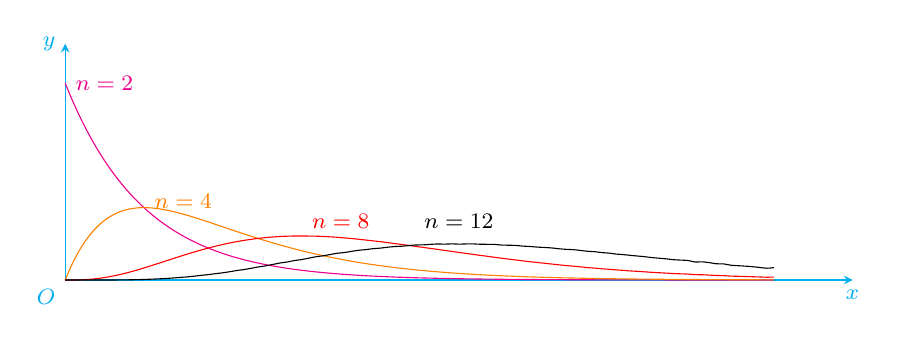
\begin{tikzpicture}[->,samples=100,>=stealth,font=\footnotesize,yscale=5,xscale=0.5]
        \def\xmin{0}
        \def\xmax{20}
        \def\ymin{0}
        \def\ymax{.6}
        \def\a{0.0104167}
        \def\b{0.000130208}
        
        \draw[->,cyan](\xmin,0)--(0,0)node[below left]{$O$}--(\xmax,0)node[below]{$x$};
        \draw[->,cyan](0,\ymin)--(0,\ymax)node[left]{$y$};
    
        \draw[domain=0:18,smooth,variable=\x,magenta,-] plot ({\x},{0.5*exp(-\x/2)}) node[magenta] at (1,0.5) {$n=2$};
        \draw[domain=0:18,smooth,variable=\x,orange,-] plot ({\x},{0.25*\x*exp(-\x/2)}) node[orange] at (3,0.2) {$n=4$};
        \draw[domain=0:18,smooth,variable=\x,red,-] plot ({\x},{\a*\x*\x*\x*exp(-\x/2)}) node[red] at (7,0.15) {$n=8$};
        \draw[domain=0:18,smooth,variable=\x,black,-] plot ({\x},{\b*\x*\x*\x*\x*\x*exp(-\x/2)}) node[black] at (10,0.15) {$n=12$};
    \end{tikzpicture}
    \caption{}
\end{figure}

\begin{theorem}
    若 $ X \sim \chi^{2}(n)$, 则
    $E(X)=n, D(X)=2 n .$
\end{theorem}

\begin{example}
    设 $X_1,X_2,\cdots,X_n,X_{n+1}$ 为总体 $X\sim N\qty(\mu,\sigma^2)$ 的简单随机样本, 且有 $$\bar{X}=\dfrac{1}{n}\displaystyle\sum_{i=1}^{n}X_i,~T=\dfrac{n}{(n+1)\sigma^2}\qty(X_{n+1}-\bar{X})^2$$
    求 $T$ 服从的分布, 并计算 $E(T)$ 和 $D(T)$.
\end{example}
\begin{errorSolution}
    由题意知 $X_{n+1}\sim N\qty(\mu,\sigma^2),~\bar{X}\sim N\qty(\mu,\dfrac{1}{n}\sigma^2)$, 且 $X_{n+1}$ 与 $\bar{X}$ 相互独立, 故 $X_{n+1}-\bar{X}\sim N\qty(0,\dfrac{n-1}{n}\sigma^2)$, \\
    \textbf{错因: }不能简单的加减法, 要从期望和方差的角度进行计算.\\
\end{errorSolution}
\begin{solution}
    由题意知 $X_{n+1}\sim N\qty(\mu,\sigma^2),~\bar{X}\sim N\qty(\mu,\dfrac{1}{n}\sigma^2)$, 且 $X_{n+1}$ 与 $\bar{X}$ 相互独立, 
    $$E\qty(X_{n+1}-\bar{X})=E(X_{n+1})-E\qty(\bar{X})=\mu-\mu=0,~D\qty(X_{n+1}-\bar{X})=D(X_{n+1})+D\qty(\bar{X})=\sigma^2+\dfrac{\sigma^2}{n}=\dfrac{n+1}{n}\sigma^2$$
    因此 $X_{n+1}-\bar{X}\sim N\qty(0,\dfrac{n+1}{n}\sigma^2)$, 则 $\dfrac{X_{n+1}-\bar{X}-0}{\sqrt{\dfrac{n+1}{n}}\sigma}\sim N(0,1)$, 两边平方有
    $$\qty(\dfrac{X_{n+1}-\bar{X}-0}{\sqrt{\dfrac{n+1}{n}}\sigma})^2=\dfrac{n}{(n+1)\sigma^2}\qty(X_{n+1}-\bar{X})^2=T\sim\chi^2(1)$$
    故 $E(T)=1,~D(T)=2.$
\end{solution}

\begin{theorem}[分布的可加性]
    设 $ X \sim \chi^{2}\left(n_{1}\right), Y \sim \chi^{2}\left(n_{2}\right) $, 且 $ X, Y $ 相互独立, 则
    $$X+Y \sim \chi^{2}\left(n_{1}+n_{2}\right) .$$
\end{theorem}

\begin{theorem}[$\chi^2$ 分布上 $ \alpha $ 分位点]
    设 $ \chi^{2} \sim \chi^{2}(n) $, 对于给定的 $ \alpha~~(0<\alpha<1) $, 满足条件
    $$P\left\{\chi^{2}>\chi_{\alpha}^{2}(n)\right\}=\int_{\chi_{\alpha}^{2}(n)}^{+\infty} f(y) \mathrm{d} y=\alpha$$
    的点 $ \chi_{\alpha}^{2}(n) $ 称为 $ \chi^{2}(n) $ 分布的上 $ \alpha $ 分位点.
\end{theorem}

\begin{example}
    已知 $(X,Y)$ 的概率密度函数为 $\displaystyle f(x,y)=\dfrac{1}{2\pi}\e^{-\frac{1}{2}\qty(x^2+y^2-2y+1)},-\infty<x,y<+\infty$, 求 $\dfrac{X^2}{(Y-1)^2}$ 服从的分布及参数.
\end{example}
\begin{solution}
    已知二维正态分布概率密度函数为 $$f(x,y)=\dfrac{1}{2\pi\sigma_1\sigma_2\sqrt{1-\rho^2}}\e^{-\frac{1}{2\qty(1-\rho^2)}\qty[\frac{(x-\mu_1)^2}{\sigma_1^2}-2\rho\frac{(x-\mu_1)(x-\mu_2)}{\sigma_1\sigma_2}+\frac{(y-\mu_2)^2}{\sigma_2^2}]}$$
    因此 $f(x,y)=\dfrac{1}{2\pi}\e^{-\frac{1}{2}\qty(x^2+y^2-2y+1)}\sim N(0,1;1,1;0)$, 故 $X\sim N(0,1),~Y\sim N(1,1)$ 且 $X,Y$ 相互独立, 那么 $\dfrac{X^2}{(Y-1)^2}\sim F(1,1).$
\end{solution}

\begin{example}
    设 $X_1,X_2$ 是来自总体 $X$ 的简单随机样本, 且 $$\bar{X}=\dfrac{1}{2}\displaystyle \sum_{i=1}^{2}X_i,S_2^2=\sum_{i=1}^{2}\qty(X-\bar{X})^2,Y=\sqrt{X_1X_2}$$
    \begin{enumerate}[label=(\arabic{*})]
        \item 若 $X$ 服从参数为 $\dfrac{1}{2}$ 的指数分布, 求 $EY$;
        \item 若 $X\sim N\qty(\mu,\sigma^2)$, 求 $E\qty[\qty(\bar{X}S_2^2)^2].$
    \end{enumerate}
\end{example}
\begin{solution}
    \begin{enumerate}[label=(\arabic{*})]
        \item $EY=E\qty(\sqrt{X_1X_2})=\qty[E\qty(\sqrt{X})]^2$, 下求 $E\sqrt{X}$, 
              \begin{flalign*}
                  E\sqrt{X}=\int_{-\infty}^{+\infty}\sqrt{x}\cdot f(x)\dd x=\int_{0}^{+\infty}\sqrt{x}\cdot\dfrac{1}{2}\e^{-\frac{1}{2}x}\dd x\xlongequal{\frac{1}{2}x=t}\sqrt{2}\int_{0}^{+\infty}\sqrt{t}\e^{-t}\dd t=\sqrt{2}\Gamma\qty(\dfrac{3}{2})=\dfrac{\sqrt{2}}{2}\Gamma\qty(\dfrac{1}{2})=\dfrac{\sqrt{2\pi}}{2}
              \end{flalign*}
              于是 $EY=\qty(\dfrac{\sqrt{2\pi}}{2})^2=\dfrac{\pi}{2}.$
        \item 因为 $\bar{X}$ 与 $S_2^2$ 相互独立, 所以
              \begin{flalign*}
                  E\qty[\qty(\bar{X}S_2^2)^2] & =E\qty(\bar{X}^2)E\qty[\qty(S_2^2)^2]=\qty[D\bar{X}+\qty(E\bar{X})^2]\qty[D\qty(S_2^2)+E^2\qty(S_2^2)]                        \\
                                              & =\qty[\dfrac{1}{n}DX+E^2X]\qty[\qty(\sigma^2)^2D\qty(\dfrac{S_2^2}{\sigma^2})+\qty(\sigma^2E\qty(\dfrac{S_2^2}{\sigma^2}))^2] \\
                                              & =\qty(\dfrac{1}{2}\sigma^2+\mu^2)\qty(2\sigma^4+\sigma^4)=3\sigma^4\qty(\dfrac{1}{2}\sigma^2+\mu^2).
              \end{flalign*}
    \end{enumerate}
\end{solution}

\subsection{\texorpdfstring{$t$}. 分布}

\begin{definition}[$t$ 分布]
    设随机变量 $ X \sim N(0,1), Y \sim \chi^{2}(n)$, 且 $ X, Y $ 相互独立, 则称随机变量
    $$T=\frac{X}{\sqrt{Y / n}}$$
    服从自由度为 $ n $ 的 $ t $ 分布, 记为 $ T \sim t(n) .$
\end{definition}

\begin{theorem}
    $ t $ 分布的概率密度函数 $ h(t) $ 为偶函数, 即 $ t_{1-\alpha}(n)=-t_{\alpha}(n) .$
\end{theorem}

\begin{theorem}
    当 $ n $ 足够大时, $t $ 分布近似于 $ N(0,1) $ 分布.
\end{theorem}
\begin{theorem}[$t$ 分布与 $F$ 分布]
    $ t^{2} \sim F(1, n) .$
\end{theorem}

\begin{definition}[$t $ 分布上 $ \alpha $ 分位点]
    设 $ t \sim t(n) $, 对于给定的 $ \alpha~~(0<\alpha<1) $, 满足条件
    $$P\left\{t>t_{\alpha}(n)\right\}=\int_{t_{\alpha}(n)}^{+\infty} h(t) \mathrm{d} t=\alpha$$
    的点 $ t_{\alpha}(n) $ 称为 $ t(n) $ 分布的上 $ \alpha $ 分位点.
\end{definition}

\begin{example}
    设 $(X_1, X_2, X_3)$ 为总体 $X\sim N\qty(0,\sigma^2)$ 的简单随机样本, 则统计量 $U=\dfrac{X_1-X_2}{\sqrt{2}|X_3|}$ 服从的分布为 
    \begin{tasks}(4)
        \task $t(1)$
        \task $t(2)$
        \task $F(1,1)$
        \task $F(2,1)$
    \end{tasks}
\end{example}
\begin{solution}
    第一步找出分子上的标准正态分布, 由题意 $\dfrac{X_1-X_2}{\sqrt{2}\sigma}\sim N(0,1)$,
    第二步找出分母上的卡方分布, $\qty(\dfrac{X_3}{\sigma})\sim \chi^2(1)$,
    第三步写出 $t$ 分布 $$
    \dfrac{\dfrac{X_1-X_2}{\sqrt{2}\sigma}}{\sqrt{\dfrac{\qty(\dfrac{X_3}{\sigma})^2}{1}}}=\dfrac{X_1-X_2}{\sqrt{2}\sigma\cdot\qty|\dfrac{X_3}{\sigma}|}\xlongequal{\sigma>0}\dfrac{X_1-X_2}{\sqrt{2}|X_3|}\sim t(1)
    $$
    因此选 A.
\end{solution}

\subsection{\texorpdfstring{$F$}. 分布}

\begin{definition}[$F$ 分布]
    设随机变量 $ X \sim \chi^{2}\left(n_{1}\right), Y \sim \chi^{2}\left(n_{2}\right)$, 且 $ X, Y $ 相互独立, 则称随机变量
    $$F=\frac{X / n_{1}}{Y / n_{2}}$$
    服从自由度为 $ \left(n_{1}, n_{2}\right) $ 的 $ F $ 分布, 记为 $ F \sim F\left(n_{1}, n_{2}\right)$ .
\end{definition}

\begin{theorem}
    若 $ F \sim F\left(n_{1}, n_{2}\right) $, 则有 $ \dfrac{1}{F} \sim F\left(n_{2}, n_{1}\right) ,~F_{1-\alpha}\left(n_{1}, n_{2}\right)=\dfrac{1}{F_{\alpha}\left(n_{2}, n_{1}\right)}$.
\end{theorem}

\begin{theorem}[$F $ 分布上 $ \alpha $ 分位点]
    设 $ F \sim F\left(n_{1}, n_{2}\right) $, 对于给定的 $ \alpha(0<\alpha<1) $, 满足条件
    $$P\left\{F>F_{\alpha}\left(n_{1}, n_{2}\right)\right\}=\int_{F_{\alpha}\left(n_{1}, n_{2}\right)}^{+\infty} \psi(y) \mathrm{d} y=\alpha$$
    的点 $ F_{\alpha}\left(n_{1}, n_{2}\right) $ 称为 $ F\left(n_{1}, n_{2}\right) $ 分布的上 $ \alpha $ 分位点.
\end{theorem}

\begin{example}
    设随机变量 $X\sim F(2,4)$, 对任意的 $\alpha\in(0,1)$, 若 $P\qty{X\leqslant a}=\alpha$, 则 $a$ 等于
    \begin{tasks}(4)
        \task $F_\alpha(2,4)$
        \task $\dfrac{1}{F_\alpha(2,4)}$
        \task $\dfrac{1}{F_{1-\alpha}(4,2)}$
        \task $\dfrac{1}{F_\alpha(4,2)}$
    \end{tasks}
\end{example}
\begin{solution}
    由 $P\qty{X\leqslant a}=\alpha$ 得 $a=F_{1-\alpha}(2,4)$, 因为 $F_{1-\alpha}(2,4)=\dfrac{1}{F_\alpha(4,2)}$, 故 $a=\dfrac{1}{F_\alpha(4,2)}$, 选 D.
\end{solution}

\begin{example}
    设随机变量 $X\sim  N(0,4)$, $X_1, X_2, \cdots ,X_n~(n>2)$ 是来自总体 $X$ 的简单随机样本, 则 
    \begin{tasks}(2)
        \task $\displaystyle \dfrac{1}{2n}\qty(\sum_{i=1}^{n}X_i)^2\sim \chi^2(1)$
        \task $\displaystyle \dfrac{1}{16}\qty(\sum_{i=1}^{n}X_i)^2\sim \chi^2(n)$
        \task $\sqrt{\dfrac{(n-1)X_n^2}{\displaystyle \sum_{i=1}^{n} X_i^2}}\sim t(n-1)$
        \task $\dfrac{(n-1)X_1^2}{\displaystyle \sum_{i=1}^{n} X_i^2}\sim F(1,n-1)$
    \end{tasks}
\end{example}
\begin{solution}
    对 A 选项, 因为 $\dfrac{\bar{X}}{\dfrac{2}{\sqrt{n}}}\sim N(0,1)$, 其中 $\bar{X}=\dfrac{1}{n}\displaystyle \sum_{i=1}^{n} X_i$, 所以 $$\dfrac{1}{2\sqrt{n}}\displaystyle \sum_{i=1}^{n} X_i\sim N(0,1)$$ 即 $\dfrac{1}{4n}\displaystyle \sum_{i=1}^{n} X_i\sim \chi^2(1)$ A 错误;
    对 B 选项, 因为 $\dfrac{X}{2}\sim N(0,1)$, 所以 $$\displaystyle \sum_{i=1}^{n} \qty(\dfrac{X_i}{2})^2\sim \chi^2(n)$$ B 错误;
    对 C 选项, $$\displaystyle \dfrac{\dfrac{X_n}{2}}{\sqrt{\dfrac{\dfrac{1}{4}\displaystyle \sum_{i=1}^{n-1} X_i^2}{n-1}}}=\dfrac{X_n\sqrt{n-1}}{\sqrt{\displaystyle \sum_{i=1}^{n-1} X_i^2}}\sim t(n-1)$$ C 错误;
    对 D 选项, $\qty(\dfrac{1}{2}X_1)^2\sim \chi^2(1), \displaystyle \sum_{i=2}^{n} \qty(\dfrac{1}{2}X_i)^2\sim \chi^2(n-1)$, 那么 $$\dfrac{\qty(\dfrac{1}{2}X_1)^2/1}{\displaystyle \sum_{i=2}^{n}\qty(\dfrac{1}{2}X_i)^2 / (n-1)}=\dfrac{(n-1)X_1}{\displaystyle \sum_{i=2}^{n} X_i^2}\sim F(1,n-1)$$
    因此选 D.
\end{solution}

\begin{example}
    设 $X_1,X_2,\cdots,X_n$ 为来自正态总体 $N\qty(\mu,\sigma^2)$ 的简单随机样本, 则数学期望 $$E\qty{\displaystyle\qty(\sum_{i=1}^{n}X_i)\qty[\sum_{j=1}^{n}\qty(nX_j-\sum_{k=1}^{n}X_k)^2]}$$ 等于
    \begin{tasks}(4)
        \task $n^3(n-1)\mu\cdot\sigma^2$
        \task $n^2(n-1)\mu\cdot\sigma^2$
        \task $n(n-1)\mu\cdot\sigma^2$
        \task $n^3(n-1)\mu\cdot\sigma$
    \end{tasks}
\end{example}
\begin{solution}
    令 $\bar{X}=\dfrac{1}{n}\displaystyle\sum_{i=1}^{n}X_i$, 那么 $\displaystyle\sum_{i=1}^{n}X_i=n\bar{X}$, 
    $$\sum_{j=1}^{n}\qty(nX_j-\sum_{k=1}^{n}X_k)^2=\sum_{j=1}^{n}\qty(nX_j-n\bar{X})^2=n^2\sum_{j=1}^{n}\qty(X_j-\bar{X})^2=n^2(n-1)S^2$$
    因此
    $$E\qty{\displaystyle\qty(\sum_{i=1}^{n}X_i)\qty[\sum_{j=1}^{n}\qty(nX_j-\sum_{k=1}^{n}X_k)^2]}=E\qty[n\bar{X}\cdot n^2(n-1)S^2]=n^3(n-1)E\qty(\bar{X}\cdot S^2)\xlongequal{\bar{X},S^2\text{ 相互独立}}n^3(n-1)\mu\sigma^2$$
    故选 A.
\end{solution}

\begin{example}
    设 $X_1,X_2,\cdots,X_n~~(n\geqslant 2)$ 为来自总体 $N(\mu,1)$ 的简单随机样本, 及 $\bar{X}=\dfrac{1}{n}\displaystyle\sum_{i=1}^{n}X_i$, 则 不能得出结论
    \begin{tasks}(2)
        \task $\displaystyle \sum_{i=1}^{n}(X_i-\mu)^2$ 服从 $\chi^2$ 分布
        \task $\displaystyle 2(X_n-X_1)^2$ 服从 $\chi^2$ 分布
        \task $\displaystyle \sum_{i=1}^{n}\qty(X_i-\bar{X})^2$ 服从 $\chi^2$ 分布
        \task $\displaystyle n\qty(\bar{X}-\mu)^2$ 服从 $\chi^2$ 分布
    \end{tasks}
\end{example}
\begin{solution}
    $X_i-\mu\sim N(0,1)$, 由卡方分布的定义知 $\displaystyle\sum_{i=1}^{n}(X_i-\mu)^2\sim \chi^2(n)$, A 正确;
    $X_n\sim N(\mu,1),~X_1\sim N(\mu,1)$, 标准化处理有 $\dfrac{X_n-X_1}{\sqrt{2}}\sim N(0,1)$, 即 $\qty(\dfrac{X_n-X_1}{\sqrt{2}})^2\sim \chi^2(1)\Rightarrow \dfrac{\qty(X_n-X_1)^2}{2}\sim \chi^2(1)$, 故选项 B 错误;
    由于 $\displaystyle \sum_{i=1}^{n}\qty(X_i-\bar{X})^2=(n-1)S^2$, 而 $\dfrac{(n-1)S^2}{\sigma^2}\sim \chi^2(n-1)$, 则 $\dfrac{(n-1)S^2}{1}\sim \chi^2(n-1)$, 即 $\displaystyle \sum_{i=1}^{n}\qty(X_i-\bar{X})^2\sim \chi^2(n-1)$, C 正确;
    由于 $\dfrac{\bar{X}-\mu}{\sqrt{\dfrac{1}{n}}}\sim N(0,1)$, 则 $\displaystyle\qty(\dfrac{\bar{X}-\mu}{1/ \sqrt{n}})^2=n\qty(\bar{X}-\mu)^2\sim \chi^2(1)$, D 正确.
\end{solution}

\begin{example}
    已知 $(X,Y)$ 的概率密度函数为 $\displaystyle f(x,y)=\dfrac{1}{2\pi}\e^{-\frac{1}{2}\qty(x^2+y^2-2y+1)},-\infty<x,y<+\infty$, 求 $\dfrac{X^2}{(Y-1)^2}$ 服从的分布及参数.
\end{example}
\begin{solution}
    已知二维正态分布概率密度函数为 $$f(x,y)=\dfrac{1}{2\pi\sigma_1\sigma_2\sqrt{1-\rho^2}}\e^{-\frac{1}{2\qty(1-\rho^2)}\qty[\frac{(x-\mu_1)^2}{\sigma_1^2}-2\rho\frac{(x-\mu_1)(x-\mu_2)}{\sigma_1\sigma_2}+\frac{(y-\mu_2)^2}{\sigma_2^2}]}$$
    因此 $f(x,y)=\dfrac{1}{2\pi}\e^{-\frac{1}{2}\qty(x^2+y^2-2y+1)}\sim N(0,1;1,1;0)$, 故 $X\sim N(0,1),~Y\sim N(1,1)$ 且 $X,Y$ 相互独立, 那么 $\dfrac{X^2}{(Y-1)^2}\sim F(1,1).$
\end{solution}

\begin{example}
    设总体 $X\sim N(0,1),~(X_1,X_2,\cdots,X_{10})$ 为 $X$ 的简单随机样本, 
    \begin{enumerate}[label=(\arabic{*})]
        \item 若 $T=\displaystyle\dfrac{1}{3}\qty(\sum_{i=1}^{3}X_i)^3+\dfrac{1}{7}\qty(\sum_{i=4}^{10}X_i)^2$, 求 $T$ 服从的分布;
        \item 若 $T=\dfrac{\displaystyle7\sum_{i=1}^{3}X_i^2}{\displaystyle 3\sum_{i=4}^{10}X_i^2}$, 求 $T$ 服从的分布;
        \item 若 $T=\dfrac{3X_1}{\sqrt{\displaystyle\sum_{i=2}^{10}X_i^2}}$, 求 $T$ 服从的分布.
    \end{enumerate}
\end{example}
\begin{solution}
    \begin{enumerate}[label=(\arabic{*})]
        \item 因为 $\displaystyle\sum_{i=1}^{3}X_i=X_1+X_2+X_3\sim N(0+0+0,1+1+1)=N(0,3)$, 所以
              $$\dfrac{1}{3}\qty(\sum_{i=1}^{3}X_i)^2=\dfrac{\displaystyle\qty(\sum_{i=1}^{3}X_i)^2}{\qty(\sqrt{3})^2}=\qty(\dfrac{\sum_{i=1}^{3}X_i-0}{\sqrt{3}})^2\sim \chi^2(1)$$
              同理 $\dfrac{1}{7}\qty(\displaystyle\sum_{i=4}^{10}X_i)^2=\dfrac{\qty(\displaystyle\sum_{i=4}^{10}X_i)^2}{\qty(\sqrt{7})^2}=\qty(\dfrac{\sum_{i=4}^{10}X_i-0}{\sqrt{7}})^2\sim\chi^2(1)$, 
              于是 $T=\displaystyle\dfrac{1}{3}\qty(\sum_{i=1}^{3}X_i)^3+\dfrac{1}{7}\qty(\sum_{i=4}^{10}X_i)^2\sim\chi^2(2).$
        \item $T=\dfrac{\displaystyle7\sum_{i=1}^{3}X_i^2}{\displaystyle 3\sum_{i=4}^{10}X_i^2}=\dfrac{\dfrac{\sum_{i=1}^{3}X_i^2}{3}}{\dfrac{\sum_{i=4}^{10}X_i^2}{7}}\sim F(3,7).$
        \item $T=\dfrac{3X_1}{\sqrt{\displaystyle\sum_{i=2}^{10}X_i^2}}=\dfrac{X_1}{\dfrac{\sqrt{\sum_{i=2}^{10}X_i^2}}{3}}=\dfrac{X_1}{\sqrt{\dfrac{\sum_{i=2}^{10}X_i^2}{9}}}\sim t(9).$
    \end{enumerate}
\end{solution}

常用分布及其数学期望与方差.
\setcounter{magicrownumbers}{0}
\begin{table}[H]
    \centering
    \caption{常用分布及其数学期望与方差}
    \resizebox{.99\textwidth}{!}{
        \begin{tabular}{l l | c c}
            \textbf{分布名称及记号}                              & \textbf{概率函数或概率密度}                                                                                                                                                                                                                                                                    & \textbf{数学期望}             & \textbf{方差}                                             \\
            \toprule
            (\rownumber) “0-1” 分布                     & $p(x)=p^xq^{1-x},~x=0,1,~0<p<1,~p+q=1$                                                                                                                                                                                                                                                & $p$                  & $pq$                                             \\
            (\rownumber) 二项分布 $B(n,p)$              & $p(x)=\C_n^xp^xq^{n-x},~x=0,1,2,\cdots,n,~0<p<1,~p+q=1$                                                                                                                                                                                                                               & $np$                 & $npq$                                            \\
            (\rownumber) 超几何分布 $H(n,M,N)$          & $p(x)=\dfrac{\C_M^x\C_{N-M}^{n-x}}{\C_N^n},~x=0,1,\cdots,\min\qty{n,M},~0\leqslant n,M\leqslant N$                                                                                                                                                                                    & \makecell[c]{$np$\\ $p=M/N$}      & $npq\dfrac{N-n}{N-1}$                 \\
            (\rownumber) 泊松分布 $\pi(\lambda)$          & $p(x)=\dfrac{\lambda^x\e^{-\lambda}}{x!},~x=0,1,2,\cdots,~\lambda>0$                                                                                                                                                                                                                  & $\lambda$            & $\lambda$                                        \\
            (\rownumber) 几何分布 $G(p)$                & $p(x)=pq^{x-1},~x=1,2,\cdots,~0<p<1,~p+q=1$                                                                                                                                                                                                                                           & $\dfrac{1}{p}$       & $\dfrac{q}{p^2}$                                 \\
            \midrule
            (\rownumber) 均匀分布 $U(a,b)$              & $f(x)=\begin{cases}\dfrac{1}{b-a},&a\leqslant x\leqslant b\\0,&\text{其他}\end{cases}$                                                                                                                                                                                                & $\dfrac{a+b}{2}$     & $\dfrac{(b-a)^2}{12}$                            \\
            (\rownumber) 指数分布 $e(\lambda)$          & $f(x)=\begin{cases}\lambda\e^{-\lambda x},&x>0\\0,&\text{其他}\end{cases}\lambda>0$                                                                                                                                                                                                   & $\dfrac{1}{\lambda}$ & $\dfrac{1}{\lambda^2}$                           \\
            (\rownumber) 正态分布 $N\qty(\mu,\sigma^2)$ & $f(x)=\dfrac{1}{\sqrt{2\pi}\sigma}\e^{-\frac{(x-\mu)^2}{2\sigma^2}},~-\infty<x+\infty,~\sigma>0$                                                                                                                                                                                      & $\mu$                & $\sigma^2$                                       \\
            \midrule
            (\rownumber) $\chi^2$ 分布 $\chi^2(k)$      & $f(x)=\begin{cases}\dfrac{x^{\frac{k}{2}-1}\e^{-\frac{x}{2}}}{2^{\frac{k}{2}}\Gamma\qty(\dfrac{k}{2})},&x>0\\0,&x\leqslant 0\end{cases}k\in\mathbb{Z}$                                                                                         & $k$                  & $2k$                                             \\
            (\rownumber) $t$ 分布 $t(k)$                & $f(x)=\dfrac{\Gamma\qty(\dfrac{k+1}{2})}{\sqrt{k\pi}\Gamma\qty(\dfrac{k}{2})}\qty(1+\dfrac{x^2}{k})^{-\frac{k+1}{2}}$                                                                                                                                                                 & \makecell[c]{$0$\\$(k>1)$}                  & \makecell[c]{$\dfrac{k}{k-2}$\\ $(k>2)$}                                 \\
            (\rownumber) $F$ 分布 $F(k_1,k_2)$          & $f(x)=\begin{cases}\dfrac{\Gamma\qty(\dfrac{k_1+k_2}{2})}{\Gamma\qty(\dfrac{k_1}{2})\Gamma\qty(\dfrac{k_2}{2})}k_1^{\frac{k_1}{2}}k_2^{\frac{k_2}{2}}\dfrac{x^{\frac{k_1}{2}-1}}{(k_1x+k_2)^{\frac{k_1+k_2}{2}}},&x>0\\0,&x\leqslant 0\end{cases}$ & \makecell[c]{$\dfrac{k_2}{k_2-2}$\\ $(k_2>2)$} & \makecell[c]{$\dfrac{2k_2^2(k_1+k_2-2)}{k_1(k_2-2)^2(k_2-4)}$\\ $(k_2>4)$}
        \end{tabular}}
\end{table}

\section{正态总体的抽样分布}

设总体 $ X $ (不管服从什么分布, 只要均值和方差存在) 的均值为 $ \mu $, 方差为 $ \sigma^{2}, X_{1}, X_{2}, \cdots ,  X_{n} $ 为来自 $ X $ 的一个样本, 样本均值 $\displaystyle \bar{X}=\frac{1}{n} \sum_{i=1}^{n} X_{i} $, 样本方差 $\displaystyle S^{2}=\frac{1}{n-1} \sum_{i=1}^{n}\left(X_{i}-\bar{X}\right)^{2} $, 则有 $\displaystyle E(\bar{X})=\mu, D(\bar{X})=\frac{\sigma^{2}}{n}, E\left(S^{2}\right)=\sigma^{2} $.

鉴于正态总体在数理统计中的重要性, 我们将不加证明地给出有关来自于正态总体样本均值及样本方差的统计量分布的结论. 这些结论将在总体参数的区间估计和假设检验问题中用到.

\subsection{单正态总体的抽样分布}

\begin{theorem}[单正态总体的抽样分布]
    设 $ X_{1}, X_{2}, \cdots, X_{n} $ 是来自正态总体 $ X \sim N\left(\mu, \sigma^{2}\right) $ 的简单随机样本, 样本均值为 $ \bar{X} $, 样本方差为 $ S^{2}$, 则
    \begin{enumerate}[label=(\arabic{*})]
        \item $\bar{X} \sim N\left(\mu, \dfrac{\sigma^{2}}{n}\right), \dfrac{\bar{X}-\mu}{\sigma / \sqrt{n}} \sim N(0,1) $;
        \item $\bar{X} $ 与 $ S^{2} $ 相互独立, 且
              $\displaystyle \dfrac{(n-1) S^{2}}{\sigma^{2}}=\dfrac{1}{\sigma^{2}} \sum_{i=1}^{n}\left(X_{i}-\bar{X}\right)^{2} \sim \chi^{2}(n-1)$;
        \item $\displaystyle \dfrac{\bar{X}-\mu}{S / \sqrt{n}} \sim t(n-1) $;
        \item $\displaystyle \dfrac{1}{\sigma^{2}} \sum_{i=1}^{n}\left(X_{i}-\mu\right)^{2} \sim \chi^{2}(n) .$
    \end{enumerate}
\end{theorem}

\subsection{双正态总体的抽样分布}

\begin{theorem}[双正态总体的抽样分布]
    设 $ X_{1}, X_{2}, \cdots, X_{n_{1}} $ 与 $ Y_{1}, Y_{2}, \cdots, Y_{n_{2}} $ 分别为来自于总体 $ X \sim N\left(\mu_{1}, \sigma_{1}^{2}\right) $ 和 $ Y \sim N\left(\mu_{2}, \sigma_{2}^{2}\right) $ 的样本, 且这两个样本相互独立. 设 $\displaystyle \bar{X}=\dfrac{1}{n_{1}} \sum_{i=1}^{n_{1}} X_{i} $, $\displaystyle \bar{Y}=\dfrac{1}{n_{2}} \sum_{i=1}^{n_{2}} Y_{i} $ 分别是两个样本的样本均值, $$\displaystyle S_{1}^{2}=\dfrac{1}{n_{1}-1} \sum_{i=1}^{n_{1}}\left(X_{i}-\bar{X}\right)^{2}, S_{2}^{2}=\dfrac{1}{n_{2}-1} \sum_{i=1}^{n_{2}}\left(Y_{i}-\bar{Y}\right)^{2}$$ 分别是两个样本的样本方差, 则有:
    \begin{enumerate}[label=(\arabic{*})]
        \item $\displaystyle \dfrac{\bar{X}-\bar{Y}-\left(\mu_{1}-\mu_{2}\right)}{\sqrt{\dfrac{\sigma_{1}^{2}}{n_{1}}+\dfrac{\sigma_{2}^{2}}{n_{2}}}} \sim N(0,1) ;$
        \item $\displaystyle \dfrac{S_{1}^{2} / S_{2}^{2}}{\sigma_{1}^{2} / \sigma_{2}^{2}} \sim F\left(n_{1}-1, n_{2}-1\right) ;$
        \item $\displaystyle \dfrac{\bar{X}-\bar{Y}-\left(\mu_{1}-\mu_{2}\right)}{S_{\mathrm{w}} \sqrt{\dfrac{1}{n_{1}}+\dfrac{1}{n_{2}}}} \sim t\left(n_{1}+n_{2}-2\right) $, 其中 $\displaystyle S_{\mathrm{w}}^{2}=\dfrac{\left(n_{1}-1\right) S_{1}^{2}+\left(n_{2}-1\right) S_{2}^{2}}{n_{1}+n_{2}-2} .$
    \end{enumerate}
\end{theorem}

\chapter{正态总体参数的区间估计与假设检验}%============================21

\begin{flushright}
    \begin{tabular}{r|||}
        \textit{“在波兰, 没有谁能考我!”于是, 传记作家问他, 那谁算你的导师呢?}\\
        \textit{他丝毫不迟疑的回答: “亨利.勒贝格!”}\\
        ——\textit{乔治·内曼}
    \end{tabular}
\end{flushright}

在统计学中, 对于正态总体参数的区间估计和假设检验是非常常见的问题. 正态总体是指总体服从正态分布的情况, 对于正态总体的参数(如均值和方差)的区间估计和假设检验有着特定的方法和步骤. 

1. 正态总体参数的区间估计: 

   均值的区间估计: 对于正态总体均值的区间估计, 常用的方法是利用样本均值和样本标准差构造置信区间. 当总体方差已知时, 可以使用正态分布进行区间估计; 当总体方差未知时, 可以使用 $t$ 分布进行区间估计. 

   方差的区间估计: 对于正态总体方差的区间估计, 可以使用卡方分布构造置信区间. 

2. 正态总体参数的假设检验: 
   均值的假设检验: 对于正态总体均值的假设检验, 常用的方法包括单样本 $t$ 检验、双样本 $t$ 检验、配对样本 $t$ 检验等. 假设检验的步骤包括设定原假设和备择假设、计算检验统计量、确定显著性水平、做出决策. 

   方差的假设检验: 对于正态总体方差的假设检验, 可以使用 $F$ 检验. 

3. 置信水平和显著性水平: 在区间估计和假设检验中, 置信水平和显著性水平是非常重要的概念. 置信水平表示我们对参数估计的信心程度, 通常取常见的置信水平有 95\%、99\% 等; 显著性水平表示拒绝原假设的程度, 通常取 0.05、0.01 等. 

4. 统计软件的应用: 对于复杂的正态总体参数的区间估计和假设检验问题, 可以使用统计软件 (如R、Python、SPSS等) 进行计算和分析, 以提高效率和准确性. 

通过对正态总体参数的区间估计和假设检验的研究, 我们可以更好地理解样本数据中的信息, 对总体参数进行推断和判断, 为决策提供统计学依据. 这些方法在实际问题分析和科学研究中有着广泛的应用. 
\section{区间估计}

区间估计是统计学中一种常用的方法, 用于估计一个参数的值在一个给定的区间内的范围.
在实际应用中, 我们往往无法得到一个参数的精确值, 而是通过收集样本数据, 利用统计方法来估计这个参数的取值范围.

\subsection{区间估计的定义}

\begin{definition}[区间估计]
    设总体 $ X $ 的分布函数为 $ F(x ; \theta)$, 含有未知参数 $ \theta \in \Theta$ ($\Theta $ 是 $ \theta $ 的取值范围), 
    对于给定的 $ \alpha(0<\alpha<1), \underline{\theta}=\underline{\theta}\left(X_{1}, X_{2}, \cdots, X_{n}\right) $ 和 $ \bar{\theta}=\bar{\theta}\left(X_{1}, X_{2}, \cdots, X_{n}\right)(\underline{\theta}<\bar{\theta}) $
    是来自 $ X $ 的样本 $ X_{1}, X_{2}, \cdots, X_{n} $ 确定的两个统计量, 若对于任意 $ \theta \in \Theta $ 满足
    $$P\left\{\underline{\theta}\left(X_{1}, X_{2}, \cdots, X_{n}\right)<\theta<\bar{\theta}\left(X_{1}, X_{2}, \cdots, X_{n}\right)\right\} \geqslant 1-\alpha$$
    则称随机区间 $ (\underline{\theta}, \bar{\theta}) $ 为\textit{参数} $ \theta $ \textit{的置信水平为} $ 1-\alpha $ \textit{的置信区间}, $\theta $ 和 $ \bar{\theta} $
    分别称为\textit{置信水平为} $ 1-\alpha $ 的双侧置信区间的\textit{置信下限}和\textit{置信上限}, $1-\alpha $ 称为\textit{置信水平}.
\end{definition}

置信水平 $ 1-\alpha $ 的含义: 在随机抽样中, 若重复抽样多次 (每次的样本容量相同), 
得到样本 $ X_{1}, X_{2}, \cdots, X_{n} $ 的多个样本值, 对应每个样本值都确定了一个置信区间 $ (\underline{\theta}, \bar{\theta}) $, 
每个这样的置信区间要么包含了 $ \theta $ 的真值, 要么不包含 $ \theta $ 的真值.

根据伯努利大数定理, 当抽样次数充分大时, 这些置信区间中包含 $ \theta $ 的真值的频率接近于置信水平 (即概率) $ 1-\alpha $, 
即在这些置信区间中包含 $ \theta $ 的真值的置信区间大约有 $ (1-\alpha) \times 100 \% $ 个, 
不包含 $ \theta $ 的真值的置信区间大约有 $ \alpha \times 100 \% $ 个.
例如, 给定 $ \alpha=0.05 $, 则置信水平是 $0.95$, 若重复抽样 $10000$ 次, 对应每次抽样都确定了一个置信区间 $ (\underline{\theta}, \bar{\theta}) $, 
则其中大约有 $9500$ 个置信区间包含 $ \theta $ 的真值, 大约有 $500$ 个置信区间不包含 $ \theta $ 的真值.
也就是说, 某一置信区间中包含 $ \theta $ 的真值的概率是 $0.95$.

\begin{example}
    已知某种袋装食盐的质量 $ X $ 服从正态分布 $ N\left(\mu, \sigma^{2}\right)$, 
    从一批食盐中随机抽取 $9$ 袋, 测得其质量 (单位: $ g $) 分别为
    $$\begin{array}{lllllllll}
            502 & 503 & 501 & 503 & 498 & 502 & 499 & 500 & 501
        \end{array}$$
    已知 $ \sigma=1 $, 求总体均值 $ \mu $ 的置信水平为 $0.95$ 的置信区间.
\end{example}
\begin{solution}
    由于统计量 $Z=\dfrac{\bar{X}-\mu}{\sigma/\sqrt{n}}\sim N(0,1)$, 按标准正态分布上 $\alpha$ 分位点的定义 (见图 \ref{alphafweidian}), 
    有 $$P\qty{\qty|\dfrac{\bar{X}-\mu}{\sigma/\sqrt{n}}|<z_{\alpha/2}}=1-\alpha$$
    即 $$P\qty{\bar{X}-z_{\alpha/2}\sigma/\sqrt{n}<\mu<\bar{X}+z_{\alpha/2}\sigma/\sqrt{n}}=1-\alpha$$
    故此置信区间为
    \begin{equation}
        \qty(\bar{X}-z_{\alpha/2}\sigma/\sqrt{n},\bar{X}+z_{\alpha/2}\sigma/\sqrt{n})
        \tag{1}
    \end{equation}
    常缩写为 $\qty(\bar{X}\pm z_{\alpha/2}\sigma/\sqrt{n})$.
\end{solution}

\begin{figure}[H]
    \centering
    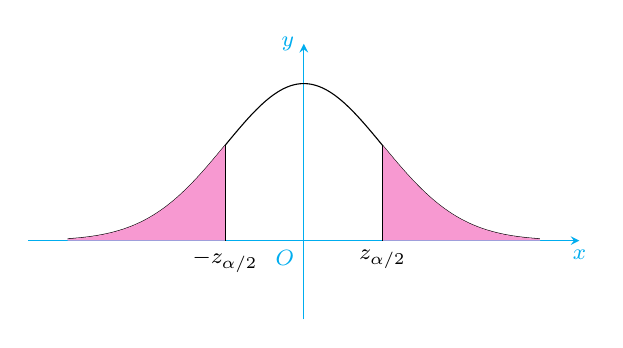
\begin{tikzpicture}[->,samples=100,>=stealth,font=\footnotesize,yscale=5]
        \def\xmin{-3.5}
        \def\xmax{3.5}
        \def\ymin{-.2}
        \def\ymax{.5}
        \def\a{0.398942}
        \draw[->,cyan](\xmin,0)--(0,0)node[below left]{$O$}--(\xmax,0)node[below]{$x$};
        \draw[->,cyan](0,\ymin)--(0,\ymax)node[left]{$y$};

        \draw[scale=1,domain=-3:3,smooth,variable=\x,black,-] plot ({\x},{\a*exp(-\x*\x/2)});

        \fill[color=magenta!40] (1,0) -- plot[domain=1:3,smooth,variable=\x] ({\x},{\a*exp(-\x*\x/2)}) -- (3,0) --cycle;
        \node[below] at (1,0) {$z_{\alpha/2}$};
        \draw[-] (1,0)--plot[domain=1:1,smooth,variable=\x] ({\x},{\a*exp(-\x*\x/2)});

        \fill[color=magenta!40] (-1,0) -- plot[domain=-1:-3,smooth,variable=\x] ({\x},{\a*exp(-\x*\x/2)}) -- (-3,0) --cycle;
        \node[below] at (-1,0) {$-z_{\alpha/2}$};
        \draw[-] (-1,0)--plot[domain=-1:-1,smooth,variable=\x] ({\x},{\a*exp(-\x*\x/2)});
    \end{tikzpicture}
    \caption{}
    \label{alphafweidian}
\end{figure}

由于 $ \alpha=0.05$, 查表知 $ z_{0.025}=1.96$, 
且由于 $ \sigma=1, n=9, \bar{x}=501 $, 由式 (1), 
得到 $ \mu $ 的置信水平为 $0.95$ 的置信区间为 $\qty(501 \pm 1.96 \times 1 / \sqrt{9}) $, 即  $(500.35,501.65)$ .

这个区间的含义是: 若反复抽样多次, 每次抽样均确定一个置信区间, 在这些置信区间中, 包含 $ \mu $ 的约占 $ 95 \% $, 
或者说某一置信区间是包含 $ \mu $ 的区间的可信程度为 $ 95 \% $.
置信区间长度的一半是 $0.65$, 表示用 $ \bar{x}=501 $ 来估计参数 $ \mu $ 的误差不大于 $0.65$, 这个误差估计的可信程度是 $ 95 \% .$

若给定置信水平 $0.99$ 时, 则 $ \alpha=0.01$, 查表知 $ z_{0.005}=2.58$, 
得到置信区间为 $ (500.14 , 501. 86)$. 可以看出, 当给定的置信水平越大时, 即 $ 1-\alpha $ 越大, 
则 $ \alpha $ 值越小, $z_{\alpha / 2} $ 越大, 从而置信区间长度 $\displaystyle 2 z_{\alpha / 2} \frac{\sigma}{\sqrt{n}} $ 越大, 
参数估计的精确程度越差.

\subsection{区间估计的一般步骤}

求置信区间的基本步骤如下:
\begin{enumerate}[label=(\arabic{*})]
    \item 选择一个与样本 $ X_{1}, X_{2}, \cdots, X_{n} $ 及 $ \theta $ 有关的函数 $ W\left(X_{1}, X_{2}, \cdots, X_{n} ; \theta\right) $, 
          使得 $ W $的分布不依赖于 $ \theta $ 和其他未知参数, 称具有这种性质的函数 $ W $ 为枢轴量.
          枢轴量选取的标准为:
          \begin{enumerate}
              \item 必须含有要估计的参数 $ \theta $, 不含有其他未知参数;
              \item 尽量使用总体的已知信息.
          \end{enumerate}
    \item 对于给定的置信水平 $ 1-\alpha$, 根据 $\displaystyle P\left\{a<W\left(X_{1}, X_{2}, \cdots, X_{n} ; \theta\right)<b\right\}=1-\alpha $, 
          在枢轴量 $ W $ 为常用分布的情况下, $a$ 和 $ b $ 可由分位数表查得.

          选择分位数 $ a $ 和 $ b $ 的标准是使区间 $ (a, b) $ 最小, 实际应用中很难实现这一点, 因此通常选取 $ a $ 和 $ b $ 使得
          $\displaystyle P\left\{W\left(X_{1}, X_{2}, \cdots, X_{n} ; \theta\right) \leqslant a\right\}=P\left\{W\left(X_{1}, X_{2}, \cdots, X_{n} ; \theta\right) \geqslant b\right\}=\alpha / 2 .$
    \item 由 $ a<W\left(X_{1}, X_{2}, \cdots, X_{n} ; \theta\right)<b$, 作恒等变形后解出参数 $ \theta $ 的取值范围, 即为所求的置信区间 $ (\underline{\theta}, \bar{\theta}) $.
    \item 代人已知样本数据进行计算.
\end{enumerate}

\section{正态总体均值和方差的区间估计}

\subsection{单个正态总体参数的置信区间}

正态总体 $ N\left(\mu, \sigma^{2}\right) $ 是最常见的分布,
下面我们讨论它的两个参数 $ \mu $ 和 $ \sigma^{2} $ 的置信区间.
设 $ X_{1}, X_{2}, \cdots, X_{n} $ 是来自总体 $ X $ 的样本.
\begin{theorem}[$\sigma^{2} $ 已知时 $ \mu $ 的置信区间]
    $\sigma^{2} $ 已知,选择枢轴量 $\displaystyle \frac{\bar{X}-\mu}{\sigma / \sqrt{n}}$,
    得到 $ \mu $ 的置信水平为 $ 1-\alpha $ 的置信区间为 $ \left(\bar{X} \pm z_{\alpha / 2} \sigma / \sqrt{n}\right) .$
\end{theorem}
\begin{theorem}[$\sigma^{2} $ 未知时 $ \mu $ 的置信区间]
    $\sigma^{2} $ 未知,由于枢轴量 $\displaystyle \frac{\bar{X}-\mu}{\sigma / \sqrt{n}} \sim N(0,1) $ 中含有未知参数 $ \sigma $,
    故不能采用. 而 $\displaystyle \frac{\bar{X}-\mu}{S / \sqrt{n}} \sim t(n-1)$ 含有待估计参数 $ \mu $,
    且不含有其他未知参数,则使用 $\displaystyle \frac{\bar{X}-\mu}{S / \sqrt{n}} $ 作为枢轴量 (见图 \ref{tfweidian}(a)), 得
    $$P\left\{-t_{\alpha / 2}(n-1)<\frac{\bar{X}-\mu}{S / \sqrt{n}}<t_{\alpha / 2}(n-1)\right\}=1-\alpha$$
    即
    $$P\left\{\bar{X}-t_{\alpha / 2}(n-1) S / \sqrt{n}<\mu<\bar{X}+t_{\alpha / 2}(n-1) S / \sqrt{n}\right\}=1-\alpha$$
    因此,$\mu $ 的置信水平为 $ 1-\alpha $ 的置信区间为
    $$\left(\bar{X}-t_{\alpha / 2}(n-1) S / \sqrt{n}, \bar{X}+t_{\alpha / 2}(n-1) S / \sqrt{n}\right)$$
    常缩写为 $$\left(\bar{X} \pm t_{a / 2}(n-1) S / \sqrt{n}\right) .$$
\end{theorem}

\begin{figure}[H]
    \centering
    \subfigure[]{
        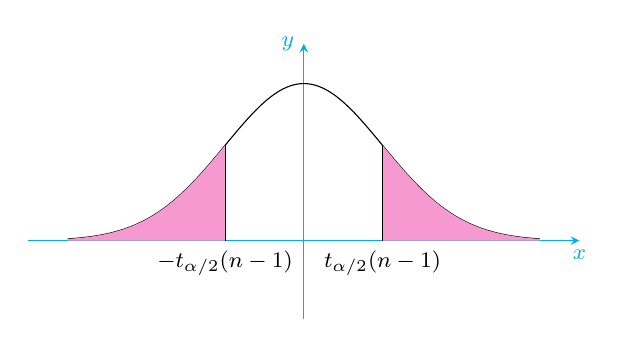
\begin{tikzpicture}[->,samples=100,>=stealth,font=\footnotesize,yscale=5]
            \def\xmin{-3.5}
            \def\xmax{3.5}
            \def\ymin{-.2}
            \def\ymax{.5}
            \def\a{0.398942}
            \draw[->,cyan](\xmin,0)--(0,0)--(\xmax,0)node[below]{$x$};
            \draw[->,cyan](0,\ymin)--(0,\ymax)node[left]{$y$};

            \draw[scale=1,domain=-3:3,smooth,variable=\x,black,-] plot ({\x},{\a*exp(-\x*\x/2)});

            \fill[color=magenta!40] (1,0) -- plot[domain=1:3,smooth,variable=\x] ({\x},{\a*exp(-\x*\x/2)}) -- (3,0) --cycle;
            \node[below] at (1,0) {$t_{\alpha/2}(n-1)$};
            \draw[-] (1,0)--plot[domain=1:1,smooth,variable=\x] ({\x},{\a*exp(-\x*\x/2)});

            \fill[color=magenta!40] (-1,0) -- plot[domain=-1:-3,smooth,variable=\x] ({\x},{\a*exp(-\x*\x/2)}) -- (-3,0) --cycle;
            \node[below] at (-1,0) {$-t_{\alpha/2}(n-1)$};
            \draw[-] (-1,0)--plot[domain=-1:-1,smooth,variable=\x] ({\x},{\a*exp(-\x*\x/2)});
        \end{tikzpicture}
    }
    \subfigure[]{
        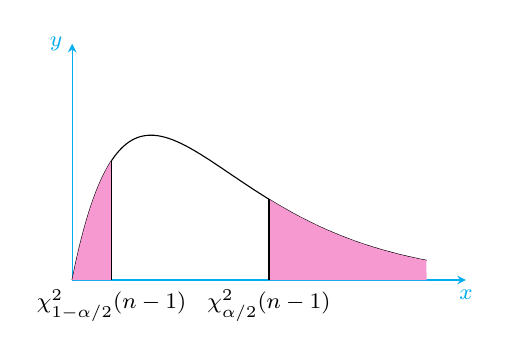
\begin{tikzpicture}[->,samples=100,>=stealth,font=\footnotesize,yscale=10,xscale=0.5]
            \def\xmin{0}
            \def\xmax{10}
            \def\ymin{0}
            \def\ymax{.3}

            \draw[->,cyan](\xmin,0)--(0,0)--(\xmax,0)node[below]{$x$};
            \draw[->,cyan](0,\ymin)--(0,\ymax)node[left]{$y$};

            \draw[domain=0:9,smooth,variable=\x,black,-] plot ({\x},{0.25*\x*exp(-\x/2)});

            \fill[color=magenta!40] (0,0) -- plot[domain=0:1,smooth,variable=\x] ({\x},{0.25*\x*exp(-\x/2)}) -- (1,0) --cycle;
            \fill[color=magenta!40] (5,0) -- plot[domain=5:9,smooth,variable=\x] ({\x},{0.25*\x*exp(-\x/2)}) -- (9,0) --cycle;

            \draw[-] (1,0) -- plot[domain=1:1,smooth,variable=\x] ({\x},{0.25*\x*exp(-\x/2)});
            \draw[-] (5,0) -- plot[domain=5:5,smooth,variable=\x] ({\x},{0.25*\x*exp(-\x/2)});

            \node[below] at (1,0) {$\chi^2_{1-\alpha/2}(n-1)$};
            \node[below] at (5,0) {$\chi^2_{\alpha/2}(n-1)$};

        \end{tikzpicture}
    }
    \caption{}
    \label{tfweidian}
\end{figure}

在实际中,$\sigma^{2} $ 未知且 $ \mu $ 已知的情形是极为少见的,因此这里只讨论 $ \mu $ 未知时 $ \sigma^{2} $ 的置信区间.

\begin{theorem}[$\mu$ 未知时 $\sigma^2$ 的置信区间]
    由于 $ \mu $ 未知,枢轴量 $\displaystyle U=\frac{\bar{X}-\mu}{\sqrt{\sigma^{2} / n}} \sim N(0,1) $ 和 $\displaystyle t=\frac{\bar{X}-\mu}{S / \sqrt{n}} \sim t(n-1) $ 中都包含 $ \mu$,
    故此不能采用, 而 $\displaystyle \frac{(n-1) S^{2}}{\sigma^{2}} \sim \chi^{2}(n-1) $ 不含有其他未知参数,
    我们采用统计量 $\displaystyle \frac{(n-1) S^{2}}{\sigma^{2}} $ 作为枢轴量 (见图 \ref{tfweidian}(b)),由
    $$P\left\{\chi_{1-\alpha / 2}^{2}(n-1)<\frac{(n-1) S^{2}}{\sigma^{2}}<\chi_{\alpha / 2}^{2}(n-1)\right\}=1-\alpha$$
    即
    $$P\left\{(n-1) S^{2} / \chi_{\alpha / 2}^{2}(n-1)<\sigma^{2}<(n-1) S^{2} / \chi_{1-\alpha / 2}^{2}(n-1)\right\}=1-\alpha$$
    则方差 $ \sigma^{2} $ 的置信水平为 $ 1-\alpha $ 的置信区间为
    $$\left((n-1) S^{2} / \chi_{\alpha / 2}^{2}(n-1),(n-1) S^{2} / \chi_{1-\alpha / 2}^{2}(n-1)\right)$$
    且标准差 $ \sigma $ 的置信水平为 $ 1-\alpha $ 的置信区间为
    $$\left(\sqrt{(n-1)} S / \sqrt{\chi_{\alpha / 2}^{2}(n-1)}, \sqrt{(n-1)} S / \sqrt{\chi_{1-\alpha / 2}^{2}(n-1)}\right) .$$
\end{theorem}

\subsection{双正态总体均值差与方差比的置信区间}

% TODO

\newpage
\begin{sidewaystable}[thp]
    \captionsetup{justification=raggedright}  % Left: using raggedleft; right: using raggedright
    \caption{正态总体参数区间估计表}
    \label{normalPopulationParameterIntervalEstimationTable}
    \centering
    \resizebox{.99\textwidth}{!}{
        \begin{tabular}{cccccc}
            \textbf{总体} & \textbf{参数} & \textbf{统计量} & \textbf{双侧置信区间} & \multicolumn{2}{c}{\textbf{单侧置信区间}} \\
            \toprule
            \makecell[c]{$X\sim N\qty(\mu,\sigma_0^2)$                                                                          \\ $\sigma^2$ 已知} & $\mu$ & $Z=\dfrac{\bar{X}-\mu}{\sigma/\sqrt{n}}\sim N(0,1)$ & $\qty(\bar{X}\pm \dfrac{\sigma}{\sqrt{n}}z_{\alpha/2})$ & $\qty(-\infty,\bar{X}+\dfrac{\sigma}{\sqrt{n}}z_{\alpha})$ & $\qty(\bar{X}-\dfrac{\sigma}{\sqrt{n}}z_\alpha,+\infty)$\\
            \makecell[c]{$X\sim N\qty(\mu,\sigma^2)$                                                                            \\ $\sigma^2$ 未知} & $\mu$ & $t=\dfrac{\bar{X}-\mu}{S/\sqrt{n}}\sim t(n-1)$ & $\qty(\bar{X}\pm t_{\alpha/2}(n-1)\dfrac{S}{\sqrt{n}})$ & $\qty(-\infty,\bar{X}+t_{\alpha}(n-1)\dfrac{S}{\sqrt{n}})$ & $\qty(\bar{X}-t_{\alpha}(n-1)\dfrac{S}{\sqrt{n}},+\infty)$\\
            \makecell[c]{$X\sim N\qty(\mu,\sigma^2)$                                                                            \\ $\mu$ 未知} & $\sigma^2$ & \makecell[l]{$\chi^2=\dfrac{(n-1)S^2}{\sigma^2}$\\$\sim \chi^2(n-1)$} & $\qty(\dfrac{(n-1)S^2}{\chi^2_{\alpha/2}(n-1)},\dfrac{(n-1)S^2}{\chi^2_{1-\alpha/2}(n-1)})$ & $\qty(0,\dfrac{(n-1)S^2}{\chi^2_{1-\alpha}(n-1)})$ & $\qty(\dfrac{(n-1)S^2}{\chi^2_{\alpha}(n-1)},+\infty)$ \\
            \midrule
            \makecell[c]{$X\sim N\qty(\mu_1,\sigma_1^2)$                                                                        \\ $Y\sim N\qty(\mu_2,\sigma_2^2)$\\ $\sigma_1^2,\sigma_2^2$ 已知} & $\mu_1-\mu_2$ & \makecell[l]{$Z=\dfrac{\bar{X}-\bar{Y}-(\mu_1-\mu_2)}{\sqrt{\dfrac{\sigma_1^2}{n_1}+\dfrac{\sigma_2^2}{n_2}}}$\\$\sim N(0,1)$} & $\qty(X-Y\pm z_{\alpha/2}\sqrt{\dfrac{\sigma_1^2}{n_1}+\dfrac{\sigma_2^2}{n_2}})$ & \makecell[l]{$\left (-\infty, \bar{X}-\bar{Y}\right .$\\$\left .+z_{\alpha}\sqrt{\dfrac{\sigma_1^2}{n_1}+\dfrac{\sigma_2^2}{n_2}}\right )$} & \makecell[l]{$\left (\bar{X}-\bar{Y}\right .$\\$\left .-z_{\alpha}\sqrt{\dfrac{\sigma_1^2}{n_1}+\dfrac{\sigma_2^2}{n_2}},+\infty\right )$}\\
            \makecell[c]{$X\sim N\qty(\mu_1,\sigma^2)$                                                                          \\ $Y\sim N\qty(\mu_2,\sigma^2)$\\ $\sigma^2$ 未知} & $\mu_1-\mu_2$ & \makecell[l]{$t=\dfrac{\bar{X}-\bar{Y}-(\mu_1-\mu_2)}{S_w\sqrt{\dfrac{1}{n_1}+\dfrac{1}{n_2}}}$\\ $\sim t(n_1+n_2-2)$} & \makecell[l]{$\left ( \bar{X}-\bar{Y}+\pm t_{\alpha/2}\left (n_1+n_2\right .\right .$\\ $-2)\cdot \left .S_w\sqrt{\dfrac{1}{n_1}+\dfrac{1}{n_2}}\right )$} & \makecell[l]{$\left (-\infty,\bar{X}-\bar{Y}+t_{\alpha}\left (n_1+n_2\right .\right .$\\ $\left .-2)\cdot S_w\sqrt{\dfrac{1}{n_1}+\dfrac{1}{n_2}}\right )$} & \makecell[l]{$\left (\bar{X}-\bar{Y}-t_{\alpha}\left (n_1+n_2\right .\right .$\\ $\left .-2)\cdot S_w\sqrt{\dfrac{1}{n_1}+\dfrac{1}{n_2}},+\infty\right )$}\\
            \makecell[c]{$X\sim N\qty(\mu_1,\sigma_1^2)$                                                                        \\ $Y\sim N\qty(\mu_2,\sigma_2^2)$\\ $\mu_1,\mu_2$ 未知} & $\dfrac{\sigma_1^2}{\sigma_2^2}$ & \makecell[l]{$F=\dfrac{S_1^2/S_2^2}{\sigma_1^2/\sigma_2^2}$\\ $\sim F(n_1-1,n_2-1)$} & \makecell[l]{$\left (\dfrac{S_1^2}{S_2^2}\cdot F_{\alpha/2}^{-1}(n_1-1,n_2-1)\right .$\\ $\left .\dfrac{S_1^2}{S_2^2}\cdot F_{1-\alpha/2}^{-1}(n_1-1,n_2-1)\right )$} & $\qty(0,\dfrac{S_1^2}{S_2^2}\cdot F_{1-\alpha}^{-1}(n_1-1,n_2-1))$ & $\qty(\dfrac{S_1^2}{S_2^2}\cdot F_{\alpha}^{-1}(n_1-1,n_2-1),+\infty)$
        \end{tabular}
    }
\end{sidewaystable}
\section{单侧置信区间}

单侧置信区间是指在统计学中用于估计参数的一种区间估计方法,只考虑了参数的一个方向. 单侧置信区间通常用于确定参数的下限或上限,而不是同时确定参数的上限和下限. 

\begin{definition}[单侧置信下限]
    对于给定值 $ \alpha(0<\alpha<1), \underline{\theta}=\theta\left(X_{1}, X_{2}, \cdots, X_{n}\right) $ 是由样本 $ X_{1}, X_{2}, \cdots, X_{n}$ 确定的统计量,对于任意的 $ \theta \in \Theta $ 满足 $ P\qty{\theta>\underline{\theta}} \geqslant 1-\alpha$,称随机区间 $ (\underline{\theta},+\infty) $ 为参数 $ \theta $ 的置信水平为 $ 1-\alpha $ 的\textit{单侧置信区间},$ \theta $ 称为 $ \theta $ 的置信水平为 $ 1-\alpha $ 的\textit{单侧置信下限}.
\end{definition}

\begin{definition}[单侧置信上限]
    对于给定值 $ \alpha(0<\alpha<1), \bar{\theta}=\bar{\theta}\left(X_{1}, X_{2}, \cdots, X_{n}\right) $ 是由样本 $ X_{1}, X_{2}, \cdots, X_{n} $ 确定的统计量,对于任意的 $ \theta \in \Theta $ 满足 $ P\{\theta<\bar{\theta}\} \geqslant 1-\alpha$,称随机区间 $ (-\infty, \bar{\theta}) $ 为参数 $ \theta $ 的置信水平为 $ 1-\alpha $ 的\textit{单侧置信区间},$ \bar{\theta} $ 称为 $ \theta $ 的置信水平为 $ 1-\alpha $ 的\textit{单侧置信上限}.
\end{definition}

单侧置信上限和单侧置信下限的求法与双侧置信区间的求法类似, 步骤如下:
\begin{enumerate}[label=(\arabic{*})]
    \item 选择枢轴量的方法与双侧置信区间枢轴量的确定方法是相同的;
    \item 对于给定的置信水平 $ 1-\alpha $,若求单侧置信下限,根据 $ P\{\theta>\underline{\theta}\} \geqslant 1-\alpha $,若求单侧置信上限,根据 $ P\{\theta<\bar{\theta}\} \geqslant 1-\alpha$,求出分位数 $ \underline{\theta} $ 或者 $ \bar{\theta} $;
    \item 由 $ \theta>\underline{\theta} $ 或者 $ \theta<\bar{\theta} $,作恒等变形后解出参数 $ \theta $ 的取值范围,即所求的单侧置信区间;
    \item 代人已知样本数据进行计算,求出具体区间.
\end{enumerate}

\begin{example}
    从一批电视机中随机地抽取 $6$ 台做寿命试验,测得寿命 (单位: h) 为
    $$\begin{array}{llllll}
            24000 & 25500 & 30100 & 28530 & 30150 & 29870
        \end{array}$$
    设电视机的寿命服从正态分布,求电视机平均寿命的单侧置信下限 ($\alpha=0.1$) .
\end{example}
\begin{solution}
    设电视机的寿命 $X\sim N\qty(\mu,\sigma^2)$,$\sigma^2$ 未知,由于 $\dfrac{\bar{X}-\mu}{S/\sqrt{n}}\sim t(n-1)$ 含有待估计参数 $\mu$,且不含有其他未知参数,故使用 $\dfrac{\bar{X}-\mu}{S/\sqrt{n}}\sim t(n-1)$ 作为枢纽量,则 
    $$P\qty{\dfrac{\bar{X}-\mu}{S/\sqrt{n}}\sim t(n-1)<t_{\alpha}(n-1)}=1-\alpha$$
    即 
    $$P\qty{\mu>\bar{X}-t_{\alpha}(n-1)S/\sqrt{n}}=1-\alpha$$
    于是得到 $\mu$ 的置信水平为 $1-\alpha$ 的单侧置信下限为 $$\bar{X}-t_{\alpha}(n-1)S/\sqrt{n}$$
    根据已知数据,得 $ \bar{x}=28025, s=2647.9, n=6 , $由 $ \alpha=0.1 $,
    查表知 $ t_{\alpha}(n-1)=t_{0.1}(5)=  1.4759 $,于是得到 $ \mu $ 的置信水平为 $0.9$ 的单侧置信下限为 $ 28025-1.4759 \times 2647.9 / \sqrt{6}=  26430.$
\end{solution}
\section{假设检验}

假设检验是一种统计推断方法, 用于判断关于总体参数的某种假设是否成立. 在假设检验中, 我们通常会提出一个关于总体参数的假设, 然后利用样本数据来判断这个假设是否成立. 

\subsection{假设检验的基本思想}

\begin{example}
    某厂生产一种袋装白糖, 每袋白糖的净重是一个随机变量, 服从正态分布 $ N\left(\mu, \sigma^{2}\right)$, \label{baitjq}
    机器正常工作时, 均值是 $0.5$ (单位: $ \mathrm{kg}$), 标准差是 $ 0.01 \mathrm{~kg}$, 某天随机地抽取 $5$ 袋白糖, 称得净重为
    $$\begin{array}{lllll}
            0.54 & 0.58 & 0.47 & 0.49 & 0.52
        \end{array}$$
    问当日机器是否正常工作?
\end{example}
\begin{solution}
    由题意知, 方差 $ \sigma^{2} $ 已知, $\mu $ 未知, 要判断机器是否正常工作, 就是要判断该日生产的白糖净重的均值是否为 $ 0.5 \mathrm{~kg} $, 
    即检验假设“$\mu=0.5$”是否正确. 因此, 提出两个相互对立的假设:\\
    原假设 $ H_{0}: \mu=\mu_{0}=0.5 $, 备择假设 $ H_{1}: \mu \neq 0.5 .$\\
    如果假设 $ H_{0}: \mu=\mu_{0}=0.5 $ 为真, 那么机器正常工作; 如果假设 $ H_{1}: \mu \neq 0.5 $ 为真, 则机器工作不正常.\\
    在假设 $ H_{0}: \mu=\mu_{0}=0.5 $ 条件下, 统计量 $\displaystyle Z=\frac{\bar{X}-\mu_{0}}{\sigma / \sqrt{n}} \sim N(0,1) $, 
    由标准正态分布的分位点的定义 (见图 \ref{alphafweidian}), 知 $ P_{\mu_{0}}\left\{\left|\frac{\bar{X}-\mu_{0}}{\sigma / \sqrt{n}}\right| \geqslant z_{\alpha / 2}\right\}=\alpha $, 
    若给定 $ \alpha=0.05$, 查表知 $ z_{0.025}=1.96$, 代人样本数据: $ n=5, \bar{x}=0.52 $, 
    则 $$\displaystyle z=\frac{\bar{x}-\mu_{0}}{\sigma / \sqrt{n}}=\frac{0.52-0.5}{0.01 / \sqrt{5}}=4.47>1.96 .$$

    这说明小概率事件发生了, 所以应该拒绝假设 $ H_{0}: \mu=\mu_{0}=0.5 $, 接受备择假设 $ H_{1}: \mu \neq 0.5 $, 即机器工作不正常.
\end{solution}

\begin{definition}[接收域和拒绝域]
    上述例题中, 若 $ z $ 取值在区间 $ (-1.96,1.96) $ 范围内, 则接受假设 $ H_{0} $, 即 $ |z|<z_{\alpha / 2} $ 称为\textit{接受域}, 
    而 $ |z| \geqslant z_{\alpha / 2} $ 称为\textit{拒绝域}, $z_{\alpha / 2} $ 称为\textit{临界值}, $\displaystyle Z=\frac{\bar{X}-\mu_{0}}{\sigma / \sqrt{n}} $ 称为\textit{检验统计量}.
\end{definition}

在根据样本作推断时, 由于样本的随机性, 难免会做出错误的决定.

\begin{definition}[第一类错误]
    当原假设 $ H_{0} $ 为真时, 而做出拒绝 $ H_{0} $ 的判断, 称为犯\textit{第一类错误} (\textit{拒真错误})
\end{definition}

\begin{definition}[第二类错误]
    当原假设 $ H_{0} $ 不真时, 而作出接受 $ H_{0} $ 的判断, 称为犯\textit{第二类错误} (\textit{取伪错误}).
\end{definition}

\begin{definition}[显著性水平]
    在实际应用中, 控制犯第一类错误的概率, 使其不大于一个较小的正数 $ \alpha(0<\alpha<1)$, 称 $ \alpha $ 为检验的\textit{显著性水平}.
\end{definition}

\begin{definition}[双边备择假设与双边假设检验]
    形如 $ H_{1}: \mu \neq \mu_{0} $ 的假设, 表示 $ \mu $ 可能大于 $ \mu_{0} $, 也可能小于 $ \mu_{0}$, 称为\textit{双边备择假设};
    形如 $ H_{0}: \mu=\mu_{0} $ 的假设, 称为\textit{双边假设检验}.
\end{definition}

在实际中, 有时只关心均值是否减小. 例如某机器的生产效率问题, 此时我们应该关注的是生产时间, 时间越短越好.
对于采用新工艺来提高生产效率, 生产时间是否显著缩短的问题, 需要考虑如下假设检验:
原假设 $ H_{0}: \mu \geqslant \mu_{0}$, 备择假设 $ H_{1}: \mu<\mu_{0} .$

\begin{definition}[单边检验]
    形如 $ H_{0}: \mu \geqslant \mu_{0} $ 的假设称为\textit{左边检验}, 类似的形如 $ H_{0}: \mu \leqslant \mu_{0} $ 的假设称为\textit{右边检验}.
    左边检验和右边检验统称为\textit{单边检验}.
\end{definition}

\subsection{假设检验的解题步骤}

\begin{enumerate}[label=(\arabic{*})]
    \item 确定原假设 $H_0$ 与备择假设 $H_1$;
    \item 选择合适的检验统计量, 在原假设成立的条件下求其发布;
    \item 根据显著性水平 $\alpha$, 再原假设成立的条件下确定临界值和拒绝域;
    \item 判断是否落入拒绝域, 落入拒绝域则拒绝 $H_0$, 否则拒绝 $H_1$.
\end{enumerate}

\subsection{单个正态总体的假设检验}

\subsubsection{\texorpdfstring{$\sigma^2$}. 已知, 关于 \texorpdfstring{$\mu$}. 的检验 (\texorpdfstring{$Z$}. 检验)}

设总体 $ X \sim N\left(\mu, \sigma^{2}\right)$, 其中 $ \sigma^{2} $ 已知, 要检验假设:
\begin{enumerate}[label=(\arabic{*})]
    \item 双边检验. $ H_{0}: \mu=\mu_{0} $, 备择假设 $ H_{1}: \mu \neq \mu_{0} $, 
          由例题 \ref{baitjq} 知, 选取检验统计量为 $\displaystyle Z=\frac{\bar{X}-\mu_{0}}{\sigma / \sqrt{n}}$, 拒绝域为 $ |z| \geqslant z_{\alpha / 2} .$
    \item 右边检验. $ H_{0}: \mu \leqslant \mu_{0}, H_{1}: \mu>\mu_{0} $, 
          选择统计量 $\displaystyle Z=\frac{\bar{X}-\mu_{0}}{\sigma / \sqrt{n}} \sim N(0,1) $, 根据标准正态分布分位点的定义 (见图 \ref{biaozfweidian}(a)) 可知 $\displaystyle P_{\mu_{0}}\left\{\frac{\bar{X}-\mu_{0}}{\sigma / \sqrt{n}} \geqslant z_{\alpha}\right\}=\alpha $, 则拒绝域为 $ z \geqslant z_{\alpha} .$
    \item 左边检验. $ H_{0}: \mu \geqslant \mu_{0}, H_{1}: \mu<\mu_{0} $, 
          选取统计量 $\displaystyle  Z=\frac{\bar{X}-\mu_{0}}{\sigma / \sqrt{n}} \sim N(0,1)$, 由标准正态分布分位点的定义 (见图 \ref{biaozfweidian}(b)) 可知 $\displaystyle P_{\mu_{0}}\left\{\frac{\bar{X}-\mu_{0}}{\sigma / \sqrt{n}} \leqslant-z_{\alpha}\right\}=\alpha$, 则拒绝域为 $ z \leqslant-z_{\alpha} .$
\end{enumerate}

\begin{figure}[H]
    \centering
    \subfigure[]{
        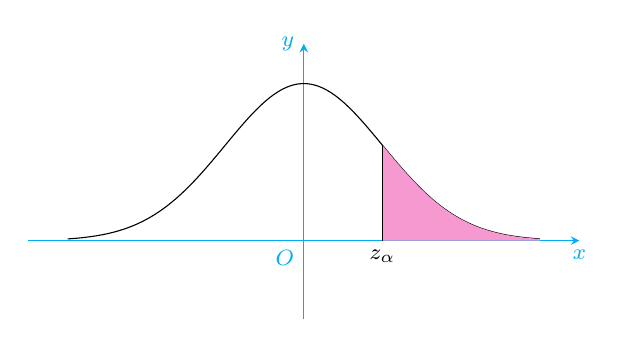
\begin{tikzpicture}[->,samples=100,>=stealth,font=\footnotesize,yscale=5]
            \def\xmin{-3.5}
            \def\xmax{3.5}
            \def\ymin{-.2}
            \def\ymax{.5}
            \def\a{0.398942}
            \draw[->,cyan](\xmin,0)--(0,0)node[below left]{$O$}--(\xmax,0)node[below]{$x$};
            \draw[->,cyan](0,\ymin)--(0,\ymax)node[left]{$y$};

            \draw[scale=1,domain=-3:3,smooth,variable=\x,black,-] plot ({\x},{\a*exp(-\x*\x/2)});

            \fill[color=magenta!40] (1,0) -- plot[domain=1:3,smooth,variable=\x] ({\x},{\a*exp(-\x*\x/2)}) -- (3,0) --cycle;
            \node[below] at (1,0) {$z_{\alpha}$};
            \draw[-] (1,0)--plot[domain=1:1,smooth,variable=\x] ({\x},{\a*exp(-\x*\x/2)});

            % \fill[color=magenta!40] (-1,0) -- plot[domain=-1:-3,smooth,variable=\x] ({\x},{\a*exp(-\x*\x/2)}) -- (-3,0) --cycle;
            % \node[below] at (-1,0) {$-z_{\alpha/2}$};
            % \draw[-] (-1,0)--plot[domain=-1:-1,smooth,variable=\x] ({\x},{\a*exp(-\x*\x/2)});
        \end{tikzpicture}
    }
    \subfigure[]{
        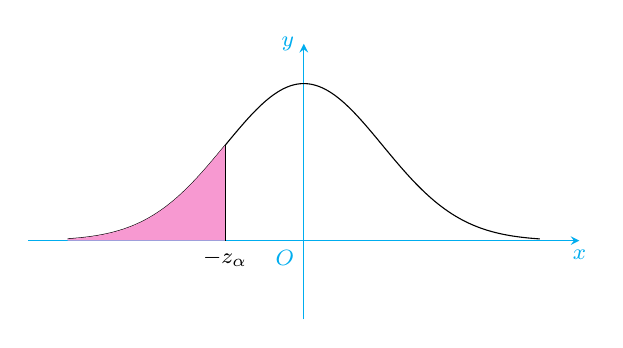
\begin{tikzpicture}[->,samples=100,>=stealth,font=\footnotesize,yscale=5]
            \def\xmin{-3.5}
            \def\xmax{3.5}
            \def\ymin{-.2}
            \def\ymax{.5}
            \def\a{0.398942}
            \draw[->,cyan](\xmin,0)--(0,0)node[below left]{$O$}--(\xmax,0)node[below]{$x$};
            \draw[->,cyan](0,\ymin)--(0,\ymax)node[left]{$y$};

            \draw[scale=1,domain=-3:3,smooth,variable=\x,black,-] plot ({\x},{\a*exp(-\x*\x/2)});

            % \fill[color=magenta!40] (1,0) -- plot[domain=1:3,smooth,variable=\x] ({\x},{\a*exp(-\x*\x/2)}) -- (3,0) --cycle;
            % \node[below] at (1,0) {$z_{\alpha/2}$};
            % \draw[-] (1,0)--plot[domain=1:1,smooth,variable=\x] ({\x},{\a*exp(-\x*\x/2)});

            \fill[color=magenta!40] (-1,0) -- plot[domain=-1:-3,smooth,variable=\x] ({\x},{\a*exp(-\x*\x/2)}) -- (-3,0) --cycle;
            \node[below] at (-1,0) {$-z_{\alpha}$};
            \draw[-] (-1,0)--plot[domain=-1:-1,smooth,variable=\x] ({\x},{\a*exp(-\x*\x/2)});
        \end{tikzpicture}
    }
    \caption{}
    \label{biaozfweidian}
\end{figure}

\begin{example}
    设某电子产品平均寿命 $ 5000 \mathrm{~h} $ 为达到标准, 现从一大批产品中抽出 $5$ 件, 试验结果 (单位: h) 如下:
    $$\begin{array}{lllll}
            5325 & 4878 & 4638 & 5652 & 4474
        \end{array}$$
    假设该产品的寿命 $ X \sim N(\mu, 1000)$, 试问此批产品是否合格 (取显著性水平 $ \alpha=0.05$)?
\end{example}
\begin{solution}
    由题意知, 需要检验假设
    $$H_0:\mu\geqslant 5000,~H_1:\mu<5000$$
    根据已知样本数据, 得 $ n=5, \bar{x}=4993, \sigma_{0}=\sqrt{1000} $, 则
    $$z=\frac{\bar{x}-\mu_{0}}{\sigma_{0} / \sqrt{n}}=\frac{\sqrt{5}(4993-5000)}{\sqrt{1000}}=-0.495$$
    查表知 $ z_{0.05}=1.645 $, 由于拒绝域为 $ z \leqslant-z_{\alpha}$, 故可接受 $ H_{0}$, 即认为该批产品合格.
\end{solution}

\subsubsection{\texorpdfstring{$\sigma^2$}. 未知, 关于 \texorpdfstring{$\mu$}. 的检验 (\texorpdfstring{$t$}. 检验)}

设总体 $ X \sim N\left(\mu, \sigma^{2}\right) $, 其中 $ \mu, \sigma^{2} $ 未知, 检验假设:
\begin{enumerate}[label=(\arabic{*})]
    \item 双边检验. $ H_{0}: \mu=\mu_{0} $, 备择假设 $ H_{1}: \mu \neq \mu_{0} $;
    \item 右边检验. $ H_{0}: \mu \leqslant \mu_{0}, H_{1}: \mu>\mu_{0}$ ;
    \item 左边检验. $ H_{0}: \mu \geqslant \mu_{0}, H_{1}: \mu<\mu_{0} $;
\end{enumerate}
这里以双边检验 $ H_{0}: \mu=\mu_{0}, H_{1}: \mu \neq \mu_{0} $ 为例求拒绝域.

若总体方差 $ \sigma^{2} $ 未知, $Z $ 检验法不能使用, 因为 $\displaystyle Z=\frac{\bar{X}-\mu_{0}}{\sigma / \sqrt{n}} $ 中含未知参数 $\sigma$, 不是统计量, 所以要选择其他的统计量来进行检验.
选取统计量 $\displaystyle t=\frac{\bar{X}-\mu_{0}}{S / \sqrt{n}} $ 作为检验统计量.
由抽样分布定理知, $\displaystyle\frac{\bar{X}-\mu_{0}}{S / \sqrt{n}} \sim t(n-1)$, 当原假设 $ H_{0} $ 成立时, 有
$$P_{\mu_{0}}\left\{\left|\frac{\bar{X}-\mu_{0}}{S / \sqrt{n}}\right| \geqslant t_{a / 2}(n-1)\right\}=\alpha$$
即得拒绝域为 $\displaystyle |t|=\left|\frac{\bar{x}-\mu_{0}}{s / \sqrt{n}}\right| \geqslant t_{\alpha / 2}(n-1)$. 
类似地, 可得单边检验的拒绝域:
\begin{enumerate}[label=(\arabic{*})]
    \item 假设 $ H_{0}: \mu \leqslant \mu_{0}, H_{1}: \mu>\mu_{0}$, 其检验的拒绝域为 $ t \geqslant t_{\alpha}(n-1) $;
    \item 假设 $ H_{0}: \mu \geqslant \mu_{0}, H_{1}: \mu<\mu_{0}$, 其检验的拒绝域为 $ t \leqslant-t_{\alpha}(n-1) $.
\end{enumerate}
这种利用 $ t $ 统计量得出的检验法称为 $ t $ 检验法.

\begin{example}
    已知钢筋强度服从正态分布, 现测得生产出的钢筋强度 (单位: $ \mathrm{Pa} $) 分别为
    $$\begin{array}{lllll}
            55.5 & 59.0 & 53.5 & 51.5 & 56.0
        \end{array}$$
    能否认为其强度的均值为 $ 52.0(\alpha=0.05) $?
\end{example}
\begin{solution}
    在 $ \sigma^{2} $ 未知的条件下, 检验假设
    $$H_{0}: \mu=52.0, \quad H_{1}: \mu \neq 52.0$$
    选择统计量 $\displaystyle t=\frac{\bar{X}-\mu_{0}}{S / \sqrt{n}}$, 
    由 $ n=5, \bar{x}=55.1, s=2.8151 $, 得统计量 $ t $ 的观测值为
    $$t=\frac{\bar{x}-\mu_{0}}{s / \sqrt{n}}=\frac{\sqrt{5}(55.1-52.0)}{2.8151}=2.4624$$
    当 $ \alpha=0.05 $, 查 $ t $ 分布表得临界值 $ t_{0.025}(4)=2.776 $, 由于 $ |t|=2.4624<2.776=t_{0.025}  (4)$, 所以接受假设 $ H_{0} $, 即认为钢笳强度的均值为 $ 52.0 $.
\end{solution}

\begin{example}
    已知某种电器在正常工作条件下平均消耗电流不会超过 $ 0.8 \mathrm{~A} $. 
    现随机抽取 $16$ 台这种电器进行试验, 求得平均消耗电流为 $ 0.91 \mathrm{~A} $, 消耗电流的标准差为 $ 0.2 \mathrm{~A}$. 
    假设电器所消耗的电流服从正态分布, 显著性水平为 $ \alpha=0.05$, 问能否认为电器在正常工作条件下平均消耗电流不会超过 $ 0.8 \mathrm{~A}$?
\end{example}
\begin{solution}
    根据题意, 检验假设
    $$H_{0}: \mu \leqslant 0.8, \quad H_{1}: \mu>0.8$$
    由于 $ \sigma $ 未知, 故采用 $ t $ 检验法, 选择检验统计量 $\displaystyle t=\frac{\bar{X}-\mu}{S / \sqrt{16}} \sim t(15) $, 
    查表得 $ t_{0.05}(15)=  1.753$, 故拒绝域为 $\displaystyle \frac{\bar{x}-0.8}{s / \sqrt{n}}>1.753 $, 代人样本数据, 得 $\displaystyle t=\frac{\bar{x}-0.8}{s / \sqrt{n}}=\frac{0.9-0.8}{0.2 / \sqrt{16}}=2 $, 因此拒绝原假设, 即认为电器在正常工作条件下平均消耗电流会超过  $0.8 \mathrm{~A}$ .
\end{solution}

\subsubsection{\texorpdfstring{$\mu$}. 未知, 关于 \texorpdfstring{$\sigma^2$}. 的检验 (\texorpdfstring{$\chi^2$}. 检验)}

设总体 $ X \sim N\left(\mu, \sigma^{2}\right), \mu, \sigma^{2} $ 均未知, $X_{1}, X_{2}, \cdots, X_{n} $ 是来自 $ X $ 的样本, 要求检验假设 $ H_{0}: \sigma^{2}=\sigma_{0}^{2} ; H_{1}: \sigma^{2} \neq \sigma_{0}^{2}, \sigma_{0}^{2} $ 为已知常数 (显著性水平为 $ \alpha $).

选取 $\displaystyle \chi^{2}=\frac{(n-1) S^{2}}{\sigma_{0}^{2}} $ 作为检验统计量, 原假设 $ H_{0} $ 成立时, $\displaystyle \frac{(n-1) S^{2}}{\sigma_{0}^{2}} \sim \chi^{2}(n-1)$, 其拒绝域的形式为 $\displaystyle \frac{(n-1) s^{2}}{\sigma_{0}^{2}} \leqslant k_{1} $ 或 $\displaystyle \frac{(n-1) s^{2}}{\sigma_{0}^{2}} \geqslant k_{2} $, 其中 $ k_{1}, k_{2} $ 由下式确定:
$$\text{由 }  P\left\{ \right. \text{拒绝 }  H_{0} \mid H_{0} \left.  \text{ 为真}  \right\}=P_{\delta_{0}}\left\{\left(\frac{(n-1) S^{2}}{\sigma_{0}^{2}} \leqslant k_{1}\right) \cup\left(\frac{(n-1) S^{2}}{\sigma_{0}^{2}} \geqslant k_{2}\right)\right\}=\alpha$$
为计算方便, 习惯上取 $\displaystyle P_{\delta_{0}}\left\{\frac{(n-1) S^{2}}{\sigma_{0}^{2}} \leqslant k_{1}\right\}=\frac{\alpha}{2},~ P_{\delta_0}\left\{\frac{(n-1) S^{2}}{\sigma_{0}^{2}} \geqslant k_{2}\right\}=\frac{\alpha}{2} $, 得 $$ k_{1}=\chi_{1-\alpha / 2}^{2}(n-1) ,~  k_{2}=\chi_{\alpha / 2}^{2}(n-1) $$
于是拒绝域为
$$\frac{(n-1) s^{2}}{\sigma_{0}^{2}} \leqslant \chi_{1-\alpha / 2}^{2}(n-1) \quad \text { 或 } \quad \frac{(n-1) s^{2}}{\sigma_{0}^{2}} \geqslant \chi_{\alpha / 2}^{2}(n-1) .$$

类似地可得关于方差的两个单边检验的拒绝域:

\begin{enumerate}[label=(\arabic{*})]
    \item 假设 $ H_{0}: \sigma^{2} \leqslant \sigma_{0}^{2} ; H_{1}: \sigma^{2}>\sigma_{0}^{2} $, 该检验的拒绝域为 $\displaystyle \frac{(n-1) s^{2}}{\sigma_{0}^{2}} \geqslant \chi_{\alpha}^{2}(n-1) $;
    \item 假设 $ H_{0}: \sigma^{2} \geqslant \sigma_{0}^{2} ; H_{1}: \sigma^{2}<\sigma_{0}^{2} $, 该检验的拒绝域为 $\displaystyle \frac{(n-1) s^{2}}{\sigma_{0}^{2}} \leqslant \chi_{1-\alpha}^{2}(n-1) $.
\end{enumerate}
以上检验法称为 $ \chi^{2} $ 检验法.

\begin{example}
    某厂应用新工艺对加工好的 $15 $ 个活塞的直径进行测量, 得样本方差 $ s^{2}=  0.0006$. 
    已知老工艺生产的活塞直径的方差为 $0.0004$. 问改革后活塞直径的方差是否不大于改革前的方差 (取显著性水平 $ \alpha=0.05$)?
\end{example}
\begin{solution}
    对方差进行右边检验, 且正态总体均值未知, 用 $ \chi^{2} $ 检验法. 
    设测量值 $ X \sim N\left(\mu, \sigma^{2}\right), \sigma^{2}=0.0004 $.
    检验假设为
    $$H_{0}: \sigma^{2} \leqslant 0.0004, \quad H_{1}: \sigma^{2}>0.0004 $$
    选择统计量 $\displaystyle \chi^{2}=\frac{(n-1) S^{2}}{\sigma_{0}^{2}} $, 拒绝域为 $ \chi^{2} \geqslant \chi_{\alpha}^{2}(n-1) $. 
    查表得 $ \chi_{0.05}^{2}(14)=23.685$, 代人样本数据, 得 $$\displaystyle \chi^{2}=\frac{(15-1) \times 0.0006}{0.0004}=21<23.685 $$ 
    故接受 $ H_{0} $, 即改革后活塞直径的方差不显著大于改革前的方差.
\end{solution}

\subsection{双正态总体的假设检验}

%TODO

\subsubsection{双正态总体均值的检验 (\texorpdfstring{$t$}. 检验)}

\subsubsection{双正态总体方差的假设检验}

正态总体方差的假设检验各情况表.
\setcounter{magicrownumbers}{0}
\begin{table}[H]
    \centering
    \resizebox{.99\textwidth}{!}{
        \begin{tabular}{cccll}
            \textbf{条件}                                 & \textbf{原假设}                      & \textbf{统计量}                                                                                                   & \textbf{对应样本函数分布}                                                        & \textbf{拒绝域}                          \\
            \toprule
            \multicolumn{5}{c}{单正态总体均值和方差的假}                                                                                                                                                                                                                                                                                           \\
            \midrule
            \multirow{3}{*}{已知 $\sigma^2$}              & $H_0:\mu=\mu_0$                      & \multirow{3}{*}{$Z=\dfrac{\bar{X}-\mu_0}{\sigma/\sqrt{n}}$}                                                       & \multirow{3}{*}{$N(0,1)$}                                                        & $|z|\geqslant z_{\alpha/2}$              \\
                                                          & $H_0:\mu\leqslant \mu_0$             &                                                                                                                   &                                                                                  & $z\geqslant z_\alpha$                    \\
                                                          & $H_0:\mu\geqslant \mu_0$             &                                                                                                                   &                                                                                  & $z\leqslant -z_\alpha $                  \\
            \midrule
            \multirow{3}{*}{未知 $\sigma^2$}              & $H_0:\mu=\mu_0$                      & \multirow{3}{*}{$t=\dfrac{\bar{X}-\mu_0}{S/\sqrt{n}}$}                                                            & \multirow{3}{*}{$t(n-1)$}                                                        & $|t|\geqslant t_{\alpha/2}(n_1+n_2-2)$   \\
                                                          & $H_0:\mu\leqslant \mu_0$             &                                                                                                                   &                                                                                  & $t\geqslant t_{\alpha}(n_1+n_2-2)$       \\
                                                          & $H_0:\mu\geqslant \mu_0$             &                                                                                                                   &                                                                                  & $t\leqslant -t_{\alpha}(n_1+n_2-2)$      \\
            \midrule
            \multirow{3}{*}{未知 $\mu$}                   & $H_0:\sigma^2=\sigma_0^2$            & \multirow{3}{*}{$\chi^2=\dfrac{(n-1)S^2}{\sigma_0^2}$}                                                            & \multirow{3}{*}{$\chi^2(n-1)$}                                                   & $\chi^2\geqslant \chi^2_{\alpha/2}(n-1)$ \\
                                                          & $H_0:\sigma^2\leqslant \sigma_0^2$   &                                                                                                                   &                                                                                  & $\chi^2\geqslant \chi^2_\alpha(n-1)$     \\
                                                          & $H_0:\sigma^2\geqslant \sigma_0^2$   &                                                                                                                   &                                                                                  & $\chi^2\leqslant \chi^2_{1-\alpha}(n-1)$ \\
            \midrule
            \multicolumn{5}{c}{双正态总体均值和方差的假}                                                                                                                                                                                                                                                                                           \\
            \midrule
            \multirow{3}{*}{已知 $\sigma_1^2,\sigma_2^2$} & $H_0:\mu_1-\mu_2=\delta$             & \multirow{3}{*}{$Z=\dfrac{\qty(\bar{X}-\bar{Y})-\sigma}{\sqrt{\dfrac{\sigma_1^2}{n_1}+\dfrac{\sigma_2^2}{n_2}}}$} & \multirow{3}{*}{$N(0,1)$}                                                        & $|z|\geqslant z_{\alpha/2}$              \\
                                                          & $H_0:\mu_1-\mu_2\leqslant \delta$    &                                                                                                                   &                                                                                  & $z\geqslant z_\alpha$                    \\
                                                          & $H_0:\mu_1-\mu_2\geqslant \delta$    &                                                                                                                   &                                                                                  & $z\leqslant -z_\alpha $                  \\
            \midrule
            \multirow{3}{*}{未知 $\sigma_1^2=\sigma_2^2$} & $H_0:\mu_1-\mu_2=\delta$             & \multirow{3}{*}{$t=\dfrac{\qty(\bar{X}-\bar{Y})-\delta}{S_w\sqrt{\dfrac{1}{n_1}+\dfrac{1}{n_2}}}$}                & \multirow{3}{*}{$t(n_1+n_2-2)$}                                                  & $|t|\geqslant t_{\alpha/2}(n_1+n_2-2)$   \\
                                                          & $H_0:\mu_1-\mu_2\leqslant \delta$    &                                                                                                                   &                                                                                  & $t\geqslant t_{\alpha}(n_1+n_2-2)$       \\
                                                          & $H_0:\mu_1-\mu_2\geqslant \delta$    &                                                                                                                   &                                                                                  & $t\leqslant -t_{\alpha}(n_1+n_2-2)$      \\
            \midrule
            \multirow{3}{*}{未知 $\mu_1,\mu_2$}           & $H_0:\sigma_1^2=\sigma_2^2$          & \multirow{3}{*}{$F=\dfrac{S_1^2}{S_2^2}$}                                                                         & \multirow{3}{*}{$\dfrac{S_1^2/S_2^2}{\sigma_1^2/\sigma_2^2}\sim F(n_1-1,n_2-1)$} & $F\geqslant F_{\alpha/2}(n_1-1,n_2-1)$   \\
                                                          & $H_0:\sigma_1^2\leqslant \sigma_2^2$ &                                                                                                                   &                                                                                  & $F\geqslant F_\alpha(n_1-1,n_2-1)$       \\
                                                          & $H_0:\sigma_1^2\geqslant \sigma_2^2$ &                                                                                                                   &                                                                                  & $F\leqslant F_{1-\alpha}(n_1-1,n_2-1)$
        \end{tabular}}
\end{table}


\section{单个正态总体的假设检验}

\subsection{\texorpdfstring{$\sigma^2$}. 已知,关于 \texorpdfstring{$\mu$}. 的检验 (\texorpdfstring{$Z$}. 检验)}


\section{双正态总体的假设检验}

\subsection{双正态总体均值的检验 (\texorpdfstring{$t$}. 检验)}

\subsection{双正态总体方差的假设检验}

正态总体方差的假设检验各情况表.
\setcounter{magicrownumbers}{0}
\begin{table}[H]
    \centering
    \resizebox{.99\textwidth}{!}{
        \begin{tabular}{cccll}
            \textbf{条件}                                 & \textbf{原假设}                      & \textbf{统计量}                                                                                                   & \textbf{对应样本函数分布}                                                        & \textbf{拒绝域}                          \\
            \toprule
            \multicolumn{5}{c}{单正态总体均值和方差的假}                                                                                                                                                                                                                                                                                           \\
            \midrule
            \multirow{3}{*}{已知 $\sigma^2$}              & $H_0:\mu=\mu_0$                      & \multirow{3}{*}{$Z=\dfrac{\bar{X}-\mu_0}{\sigma/\sqrt{n}}$}                                                       & \multirow{3}{*}{$N(0,1)$}                                                        & $|z|\geqslant z_{\alpha/2}$              \\
                                                          & $H_0:\mu\leqslant \mu_0$             &                                                                                                                   &                                                                                  & $z\geqslant z_\alpha$                    \\
                                                          & $H_0:\mu\geqslant \mu_0$             &                                                                                                                   &                                                                                  & $z\leqslant -z_\alpha $                  \\
            \midrule
            \multirow{3}{*}{未知 $\sigma^2$}              & $H_0:\mu=\mu_0$                      & \multirow{3}{*}{$t=\dfrac{\bar{X}-\mu_0}{S/\sqrt{n}}$}                                                            & \multirow{3}{*}{$t(n-1)$}                                                        & $|t|\geqslant t_{\alpha/2}(n_1+n_2-2)$   \\
                                                          & $H_0:\mu\leqslant \mu_0$             &                                                                                                                   &                                                                                  & $t\geqslant t_{\alpha}(n_1+n_2-2)$       \\
                                                          & $H_0:\mu\geqslant \mu_0$             &                                                                                                                   &                                                                                  & $t\leqslant -t_{\alpha}(n_1+n_2-2)$      \\
            \midrule
            \multirow{3}{*}{未知 $\mu$}                   & $H_0:\sigma^2=\sigma_0^2$            & \multirow{3}{*}{$\chi^2=\dfrac{(n-1)S^2}{\sigma_0^2}$}                                                            & \multirow{3}{*}{$\chi^2(n-1)$}                                                   & $\chi^2\geqslant \chi^2_{\alpha/2}(n-1)$ \\
                                                          & $H_0:\sigma^2\leqslant \sigma_0^2$   &                                                                                                                   &                                                                                  & $\chi^2\geqslant \chi^2_\alpha(n-1)$     \\
                                                          & $H_0:\sigma^2\geqslant \sigma_0^2$   &                                                                                                                   &                                                                                  & $\chi^2\leqslant \chi^2_{1-\alpha}(n-1)$ \\
            \midrule
            \multicolumn{5}{c}{双正态总体均值和方差的假}                                                                                                                                                                                                                                                                                           \\
            \midrule
            \multirow{3}{*}{已知 $\sigma_1^2,\sigma_2^2$} & $H_0:\mu_1-\mu_2=\delta$             & \multirow{3}{*}{$Z=\dfrac{\qty(\bar{X}-\bar{Y})-\sigma}{\sqrt{\dfrac{\sigma_1^2}{n_1}+\dfrac{\sigma_2^2}{n_2}}}$} & \multirow{3}{*}{$N(0,1)$}                                                        & $|z|\geqslant z_{\alpha/2}$              \\
                                                          & $H_0:\mu_1-\mu_2\leqslant \delta$    &                                                                                                                   &                                                                                  & $z\geqslant z_\alpha$                    \\
                                                          & $H_0:\mu_1-\mu_2\geqslant \delta$    &                                                                                                                   &                                                                                  & $z\leqslant -z_\alpha $                  \\
            \midrule
            \multirow{3}{*}{未知 $\sigma_1^2=\sigma_2^2$} & $H_0:\mu_1-\mu_2=\delta$             & \multirow{3}{*}{$t=\dfrac{\qty(\bar{X}-\bar{Y})-\delta}{S_w\sqrt{\dfrac{1}{n_1}+\dfrac{1}{n_2}}}$}                & \multirow{3}{*}{$t(n_1+n_2-2)$}                                                  & $|t|\geqslant t_{\alpha/2}(n_1+n_2-2)$   \\
                                                          & $H_0:\mu_1-\mu_2\leqslant \delta$    &                                                                                                                   &                                                                                  & $t\geqslant t_{\alpha}(n_1+n_2-2)$       \\
                                                          & $H_0:\mu_1-\mu_2\geqslant \delta$    &                                                                                                                   &                                                                                  & $t\leqslant -t_{\alpha}(n_1+n_2-2)$      \\
            \midrule
            \multirow{3}{*}{未知 $\mu_1,\mu_2$}           & $H_0:\sigma_1^2=\sigma_2^2$          & \multirow{3}{*}{$F=\dfrac{S_1^2}{S_2^2}$}                                                                         & \multirow{3}{*}{$\dfrac{S_1^2/S_2^2}{\sigma_1^2/\sigma_2^2}\sim F(n_1-1,n_2-1)$} & $F\geqslant F_{\alpha/2}(n_1-1,n_2-1)$   \\
                                                          & $H_0:\sigma_1^2\leqslant \sigma_2^2$ &                                                                                                                   &                                                                                  & $F\geqslant F_\alpha(n_1-1,n_2-1)$       \\
                                                          & $H_0:\sigma_1^2\geqslant \sigma_2^2$ &                                                                                                                   &                                                                                  & $F\leqslant F_{1-\alpha}(n_1-1,n_2-1)$
        \end{tabular}}
\end{table}

\chapter{参数的点估计及其优良性}%============================22

\begin{flushright}
    \begin{tabular}{r|||}
        \textit{“数学家通常是先通过直觉来发现一个定理; }\\
        \textit{这个结果对于他首先是似然的, 然后他再着手去制造一个证明. ”}\\
        ——\textit{哈代}
    \end{tabular}
\end{flushright}

在统计学中, 参数的点估计是指利用样本数据来估计总体参数的值. 点估计是统计推断的基础, 它可以帮助我们对未知参数进行估计, 并提供关于参数的一些信息. 以下是关于参数的点估计及其优良性的一些基本概念: 

1. 点估计的定义: 点估计是指用样本数据计算出一个数值作为总体参数的估计值. 常见的点估计方法包括最大似然估计、矩估计等. 

2. 最大似然估计: 最大似然估计是一种常用的点估计方法, 它通过最大化似然函数来估计参数的值. 最大似然估计的估计量具有一些优良性质, 例如渐近正态性、一致性等. 

3. 矩估计: 矩估计是另一种常见的点估计方法, 它基于样本矩来估计总体参数. 矩估计的优良性质包括无偏性、一致性等. 

4. 优良性质: 一个好的点估计应当具有一些优良性质, 例如无偏性、有效性、一致性、渐近正态性等. 无偏性是指估计量的期望值等于真实参数的值, 有效性是指估计量的方差最小, 一致性是指估计量在样本量趋于无穷时收敛于真实参数的值, 渐近正态性是指估计量在样本量趋于无穷时服从正态分布. 

通过对参数的点估计及其优良性的研究, 我们可以更好地理解样本数据中的信息, 对总体参数进行估计, 并进行统计推断. 点估计是统计学中重要的概念, 也是实际问题分析和决策制定中不可或缺的工具. 
\section{矩估计法}

设总体 $ X $ 的分布形式已知,$\theta $ 为总体的待估参数,$X_{1}, X_{2}, \cdots, X_{n} $ 为从总体 $ X $ 中抽取的样本,
如果总体 $ X $ 的数学期望 $ E(X) $ 存在,那么 $ E(X) $ 是 $ \theta $ 的函数. 例如,在泊松分布总体 $ \pi(\lambda) $ 中,
样本一阶矩 $ E(X)=\lambda$; 在指数分布总体 $ X \sim e(\lambda) $ 中,$E(X)=\dfrac{1}{\lambda}$.
由于 $ X_{1}, X_{2}, \cdots, X_{n} $ 相互独立且与总体 $ X $ 同分布,由大数定理知,当 $ n $ 越来越大时,$\displaystyle\bar{X}=\dfrac{1}{n} \sum_{i=1}^{n} X_{i} $
依概率收玫到 $ E(X)=h(\theta) .$
要估计 $ \theta $,令
$$E(X)=\frac{1}{n} \sum_{i=1}^{n} X_{i}=\bar{X}$$
解方程 $h(\theta)=\bar{X}$,可求出 $ \theta$,此种方法所得的估计 $ \hat{\theta} $ 称为未知参数 $ \theta $ 的矩估计.

\begin{example}
    设总体 $ X \sim U(a, b)$,$ a, b $ 未知,$X_{1}, X_{2}, \cdots, X_{n} $ 为来自总体 $ X $ 的样本,$  x_{1} ,  x_{2}, \cdots, x_{n} $ 是样本值,试求 $ a, b $ 的矩估计量和矩估计值.
\end{example}
\begin{solution}
    令 $\begin{cases}
            \displaystyle E(X)=\dfrac{1}{n}\sum_{i=1}^{n}X_i=\bar{X} \\
            \displaystyle E\qty(X^2)=\dfrac{1}{n}\sum_{i=1}^{n}X_i^2
        \end{cases}$,且 $X\sim U(a,b)$,那么
    $$E(X)=\dfrac{a+b}{2},~E\qty(X^2)=D(X)+E^2(X)=\dfrac{(b-a)^2}{12}+\dfrac{(a+b)^2}{4}$$
    即 $\begin{cases}
            a+b =2\bar{X} \\
            \displaystyle b-a=2\sqrt{3}\sqrt{\dfrac{1}{n}\sum_{i=1}^{n}X_i^2-\bar{X}^2}
        \end{cases}$ 并且 $\displaystyle\dfrac{1}{n}\sum_{i=1}^{n}X_i^2-\bar{X}^2=\dfrac{1}{n}\sum_{i=1}^{n}\qty(X_i-\bar{X})^2$,
    解得矩估计量和矩估计值分别为
    $$\begin{cases}
            \displaystyle \hat{a}=\bar{X}-\sqrt{\dfrac{3}{n}\sum_{i=1}^{n}\qty(X_i-\bar{X})^2} \\
            \displaystyle \hat{b}=\bar{X}+\sqrt{\dfrac{3}{n}\sum_{i=1}^{n}\qty(X_i-\bar{X})^2},
        \end{cases}
        \begin{cases}
            \displaystyle \hat{a}=\bar{x}-\sqrt{\dfrac{3}{n}\sum_{i=1}^{n}\qty(x_i-\bar{x})^2} \\
            \displaystyle \hat{b}=\bar{x}+\sqrt{\dfrac{3}{n}\sum_{i=1}^{n}\qty(x_i-\bar{x})^2}.
        \end{cases}$$
\end{solution}

\begin{example}
    设总体 $X$ 的分布函数为 $F(x)=\begin{cases}
            1-\e ^{-(x-\theta)^2}, & x\geqslant \theta \\
            0,                     & x<\theta
        \end{cases}(\theta>0\text{ 为未知数})$,$X_1,X_2,\cdots,X_n$ 为来自总体 $X$ 的简单随机样本,$\displaystyle\bar{X}=\dfrac{1}{n}\sum_{i=1}^{n}X_i$,求 $\theta$ 的矩估计量 $\bar\theta$.
\end{example}
\begin{solution}
    总体 $ X $ 的密度函数为 $f(x)=
        \begin{cases}
            2(x-\theta) \mathrm{e}^{-(x-\theta)^{2}}, & x \geqslant \theta \\ 0, & x<\theta
        \end{cases}$,那么
    \begin{flalign*}
        E(X) & =\int_{0}^{+\infty} x \cdot 2(x-\theta) \mathrm{e}^{-(x-\theta)^{2}} \dd  x=2 \int_{\theta}^{+\infty}[(x-\theta)+\theta] \cdot(x-\theta) \mathrm{e}^{-(x-\theta)^{2}} \dd (x-\theta)                                                      \\
             & =2 \int_{0}^{+\infty} x(x+\theta) \mathrm{e}^{-x^{2}} \dd  x=2 \int_{0}^{+\infty} x^{2} \mathrm{e}^{-x^{2}} \dd  x+\theta \int_{0}^{+\infty} \mathrm{e}^{-x^{2}} \dd \left(x^{2}\right)                                                   \\
             & \xlongequal{x^{2}=t} 2 \int_{0}^{+\infty} t \mathrm{e}^{-t} \cdot \frac{1}{2 \sqrt{t}} \dd  t+\theta=\int_{0}^{+\infty} t^{\frac{1}{2}} \mathrm{e}^{-t} \dd  t+\theta=\Gamma\left(\frac{1}{2}+1\right)+\theta=\frac{\sqrt{\pi}}{2}+\theta
    \end{flalign*}
    令 $ E(X)=\bar{X} $ 得参数 $ \theta $ 的矩估计量为 $ \displaystyle\hat{\theta}=\bar{X}-\frac{\sqrt{\pi}}{2} .$
\end{solution}

\begin{example}
    设总体 $ X $ 的概率密度为
    $f(x)=\begin{cases}
            2(x-\theta) \mathrm{e}^{-(x-\theta)^{2}}, & x>\theta \\ 0, & x \leqslant \theta
        \end{cases}$
    $\left(X_{1}, X_{2}, \cdots, X_{n}\right)$ 为来自总体 $ X $ 的简单随机样本.
    \begin{enumerate}[label=(\arabic{*})]
        \item 求参数 $ \theta $ 的矩估计量;
        \item 设 $ U=\min \left\{X_{1}, X_{2}, \cdots, X_{n}\right\} $,求 $ E(U) .$
    \end{enumerate}
\end{example}
\begin{solution}
    \begin{enumerate}[label=(\arabic{*})]
        \item 与上题类似,有
              \begin{flalign*}
                  E(X) & =\int_{\theta}^{+\infty} x \cdot 2(x-\theta) \mathrm{e}^{-(x-\theta)^{2}} \dd  x \xlongequal{x-\theta=t} \int_{0}^{+\infty}(t+\theta) \cdot 2 t \mathrm{e}^{-t^{2}} \dd  t                                                                                                         \\
                       & =\int_{0}^{+\infty} 2 t^{2} \mathrm{e}^{-t^{2}} \dd  t+\theta \int_{0}^{+\infty} 2 t \mathrm{e}^{-t^{2}} \dd  t=\int_{0}^{+\infty}\left(t^{2}\right)^{\frac{1}{2}} \mathrm{e}^{-t^{2}} \dd \left(t^{2}\right)+\theta \int_{0}^{+\infty} \mathrm{e}^{-t^{2}} \dd \left(t^{2}\right) \\
                       & =\Gamma\left(\frac{1}{2}+1\right)+\theta=\frac{1}{2} \Gamma\left(\frac{1}{2}\right)+\theta=\theta+\frac{\sqrt{\pi}}{2}
              \end{flalign*}
              由 $ E(X)=\bar{X} $ 得参数 $ \theta $ 的矩估计量为 $\displaystyle\hat{\theta}=\bar{X}-\frac{\sqrt{\pi}}{2}$.
        \item 总体 $ X $ 的分布函数为 $F(x)=P\{X \leqslant x\}$,

              当 $ x<\theta $ 时,$F(x)=0$; \\
              当 $ x \geqslant \theta $ 时,$\displaystyle F(x)=\int_{\theta}^{x} 2(x-\theta) \mathrm{e}^{-(x-\theta)^{2}} \dd  x=1-\mathrm{e}^{-(x-\theta)^{2}} $,即
              $$F(x)=\begin{cases}
                      0,                              & x<\theta           \\
                      1-\mathrm{e}^{-(x-\theta)^{2}}, & x \geqslant \theta
                  \end{cases}$$
              $U $ 的分布函数为
              \begin{flalign*}
                  F_{U}(x) & =P\{U \leqslant x\}=1-P\{U>x\}=1-P\left\{X_{1}>x\right\} P\left\{X_{2}>x\right\} \cdots P\left\{X_{n}>x\right\} \\
                           & =1-[P\{X>x\}]^{n}=1-[1-F(x)]^{n}=\begin{cases}
                                                                  0,                               & x<\theta           \\
                                                                  1-\mathrm{e}^{-n(x-\theta)^{2}}, & x \geqslant \theta
                                                              \end{cases}
              \end{flalign*}
              $U$ 的密度函数为
              $$f_{U}(x)=\begin{cases}
                      0,                                           & x \leqslant \theta \\
                      2 n(x-\theta) \mathrm{e}^{-n(x-\theta)^{2}}, & x>\theta
                  \end{cases}$$
              则
              \begin{flalign*}
                  E(U) & =\int_{\theta}^{+\infty} 2 n x(x-\theta) \mathrm{e}^{-n(x-\theta)^{2}} \dd  x=\int_{\theta}^{+\infty}\left[\frac{1}{\sqrt{n}}\left[n(x-\theta)^{2}\right]^{\frac{1}{2}}+\theta\right] \mathrm{e}^{-n(x-\theta)^{2}} \dd\left[n(x-\theta)^{2}\right] \\
                       & =\int_{0}^{+\infty}\left(\frac{1}{\sqrt{n}} t^{\frac{1}{2}}+\theta\right) \mathrm{e}^{-t} \dd  t=\frac{1}{\sqrt{n}} \cdot \Gamma\left(\frac{1}{2}+1\right)+\theta=\frac{\sqrt{\pi n}}{2 n}+\theta
              \end{flalign*}
    \end{enumerate}
\end{solution}
% \section{区间估计}

% \subsection{矩估计量}

% % \begin{example}
% %     设总体 $X$ 的概率密度为 $$f(x;\theta)=\begin{cases}
% %         \dfrac{\theta ^2}{x^3}\mathrm{e}^{-\frac{\theta }{x} }&,x>0  \\
% %        0&,\text{其他}
% %        \end{cases}$$
% %        其中 $\theta$ 为未知参数且大于零, $X_1,X_2,\cdots,X_n$ 为来自总体 $X$ 的简单随机样本, 
% %        求 $\theta$ 的矩估计量.
% % \end{example}

% \begin{example}
%     设总体 $X$ 的概率密度为
%     $$f(x;\theta)=\begin{cases}
%             \dfrac{6x}{\theta^3}(\theta-x) & ,0<x<\theta  \\
%             0                              & ,\text{其他}
%         \end{cases}$$
%     $X_1,X_2,\cdots,X_n$ 为来自总体 $X$ 的简单随机样本, 求 $\theta$ 的矩估计量 $\hat{\theta} $ 以及求 $\hat{\theta} $ 的方差 $D\qty(\hat{\theta} ).$
% \end{example}
% \begin{solution}
%     由 $\displaystyle E(X)=\int_{0}^{\theta}xf(x)\dd x$ 得, 
%     $$E(X)=\int_{0}^{\theta}\dfrac{6x^2}{\theta^3}(\theta-x)\dd x=\dfrac{\theta}{2}$$
%     记 $\displaystyle\bar{X}=\dfrac{1}{n}\sum_{i=1}^{n}X_i$, 令 $\dfrac{\theta}{2}=\bar{X}$, 得 $\theta$ 的矩估计量为 $\hat{\theta}=2\bar{X}$;
%     根据方差与期望的关系 $$D(X)=E(X^2)-E^2(X)$$
%     且 $\displaystyle E(X^2)=\int_{0}^{\theta}x^2f(x)\dd x=\int_{0}^{\theta}\dfrac{6x^3}{\theta^3}(\theta-x)\dd x=\dfrac{3\theta^2}{10}$, 
%     那么 $D(X)=\dfrac{\theta^2}{20}$, 所以 $\hat{\theta}=2\bar{X}$ 的方差为
%     $$D\qty(\hat{\theta})=D\qty(2\bar{X})=4D(\bar{X})=\dfrac{4}{n}D(X)=\dfrac{\theta^2}{5n}.$$
% \end{solution}

% \subsection{置信区间}

% \begin{theorem}[单个正态总体均值和方差的置信区间]
%     设总体 $X\sim N(\mu,\sigma^2)$, 常见的置信区间有: 
%     \begin{enumerate}[label=(\arabic{*})]
%         \item 当 $\sigma^2$ 已知时, $\mu$ 的置信度为 $1-\alpha$ 的置信区间为 $\qty(\bar{X}-U_{\frac{\alpha}{2}}\dfrac{\sigma}{\sqrt{n}},\bar{X}+U_{\frac{\alpha}{2}}\dfrac{\sigma}{\sqrt{n}})$.
%         \item 当 $\sigma^2$ 未知时, $\mu$ 的置信度为 $1-\alpha$ 的置信区间为 $\qty(\bar{X}-t_{\frac{\alpha}{2}}(n-1)\dfrac{S}{\sqrt{n}},\bar{X}+t_{\frac{\alpha}{2}}(n-1)\dfrac{S}{\sqrt{n}})$.
%         \item 当 $\mu$ 已知时, $\sigma^2$ 的置信度为 $1-\alpha$ 的置信区间为 $\qty(\dfrac{\sum_{i=1}^{n}(X_i-n)^2}{\chi^2_{\frac{\alpha}{2}}(n)},\dfrac{\sum_{i=1}^{n}(X_i-n)^2}{\chi^2_{1-\frac{\alpha}{2}}(n)}).$
%         \item 当 $\mu$ 未知时, $\sigma^2$ 的置信度为 $1-\alpha$ 的置信区间为 $\qty(\dfrac{(n-1)S^2}{\chi^2_{\frac{\alpha}{2}}(n)},\dfrac{(n-1)S^2}{\chi^2_{1-\frac{\alpha}{2}}(n)})$, $\sigma$ 的置信区间为 $\qty(\sqrt{\dfrac{(n-1)S^2}{\chi^2_{\frac{\alpha}{2}}(n)}},\sqrt{\dfrac{(n-1)S^2}{\chi^2_{1-\frac{\alpha}{2}}(n)}})$.
%     \end{enumerate}
% \end{theorem}

% \begin{theorem}[两个正态总体均值差的置信区间]
%     $\qty(\bar{X}-\bar{Y}-u_{\frac{\alpha}{2}}\sqrt{\dfrac{\sigma_1^2}{n_1}+\dfrac{\sigma_2^2}{n_2}},\bar{X}-\bar{Y}+u_{\frac{\alpha}{2}}\sqrt{\dfrac{\sigma_1^2}{n_1}+\dfrac{\sigma_2^2}{n_2}}).$
% \end{theorem}

\section{极大似然估计}

极大似然估计法是参数估计使用的最广泛的方法, 最早由德国数学家 Gauss 在 1821 年提出, 
但是此法一般归功于英国统计学家 Fisher, 因为 Fisher 于 1922 年再次提出了这个思想, 并且证明了这种方法的一些性质, 
从而使得极大似然法得到更普遍的应用.

\begin{example}
    设 $X_i,~i=1,2,\cdots,n$ 为来自总体 $X\sim B(N,p)~~(0<p<1)$ 的简单随机样本, 求 $p$ 的极大似然估计量.
\end{example}
\begin{solution}
    似然函数为 $\displaystyle L(p)=\prod_{i=1}^{n} \mathrm{C}_{N}^{x_{i}} \cdot p^{x_{i}} \cdot(1-p)^{N-x_{i}} $, 两边取对数, 得
    $$\ln L(p)=\sum_{i=1}^{n} \ln C_{N}^{x_{i}}+\sum_{i=1}^{n} x_{i} \ln p+\sum_{i=1}^{n}\left(N-X_{i}\right) \ln (1-p)$$
    令 $$\frac{\mathrm{d}}{\mathrm{d} p} \ln L(p)=\frac{1}{p} \sum_{i=1}^{n} x_{i}-\frac{1}{1-p}\left(n N-\sum_{i=1}^{n} x_{i}\right)=0$$
    解得 $\displaystyle p=\frac{\displaystyle \sum_{i=1}^{n} x_{i}}{n N}=\frac{\bar{X}}{N} $, 故 $ p $ 的最大似然估计量为 $ \hat{p}=\dfrac{\bar{X}}{N} $, 
    其中 $ \displaystyle\bar{X}=\dfrac{1}{n} \sum_{i=1}^{n} X_{i} .$
\end{solution}

\begin{example}
    设总体概率函数如下, $x_1,x_2,\cdots,x_n$ 是样本, 试求未知参数的极大似然估计:
    \begin{enumerate}[label=(\arabic{*})]
        \item $\displaystyle p(x;\theta)=\sqrt{\theta}x^{\sqrt{\theta}-1},0<x<1,\theta>0;$
        \item $\displaystyle p(x;\theta)=\theta c^\theta x^{-(\theta+1)},x>c>0,\theta>1.$
    \end{enumerate}
\end{example}
\begin{solution}
    \begin{enumerate}[label=(\arabic{*})]
        \item 似然函数 $\displaystyle L(\theta)=\left( \sqrt{\theta }\right) ^{n}\left( \prod ^{n}_{i=1}x_{i}\right) ^{\sqrt{\theta }-1}$, 取对数得
              $$\ln L\left( \theta \right) =\dfrac{n}{2}\ln \theta +\left( \sqrt{\theta }-1\right) \sum ^{n}_{i=1}\ln x_{i}$$
              将 $\ln L(\theta)$ 关于 $\theta$ 求导, 并令其值为 $0$ 即得到似然函数
              $$\dfrac{\partial \ln L\left( \theta \right) }{\partial \theta }=\dfrac{n}{2\theta }+\dfrac{1}{2\sqrt{\theta }}\sum ^{n}_{i=1}x_{i}=0$$
              解得 $\displaystyle\widehat{\theta }=\left( \dfrac{1}{n}\sum ^{n}_{i=1}\ln x_{i}\right) ^{-2}$, 并且
              $$ \dfrac{\partial ^{2}\ln L\left( \theta \right) }{\partial \theta ^{2}}\bigg | _{\theta=\widehat{\theta }}= \left( -\dfrac{n}{2\theta ^{2}}-\dfrac{1}{4\theta ^{3/2}}\sum ^{n}_{i=1}\ln x_{i}\right) \bigg | _{\theta=\widehat{\theta }}=-\dfrac{3}{4n^{3}}\left( \sum ^{n}_{i=1}\ln x_{i}\right) ^{4}<0$$
              所以 $\widehat{\theta}$ 是 $\theta$ 的极大似然估计.
        \item 似然函数 $\displaystyle L(\theta)=\theta ^{n}c^{n\theta }\left( \prod ^{n}_{i=1}x_{i}\right) ^{-\left( \theta +1\right) }$, 取对数得
              $$\ln L\left( \theta \right) =n\ln \theta +n\theta \ln c-\left( \theta +1\right) \sum ^{n}_{i=1}\ln x_{i}$$
              将 $\ln L(\theta)$ 关于 $\theta$ 求导, 并令其值为 $0$ 即得到似然函数
              $$\dfrac{\partial \ln L\left( \theta \right) }{\partial \theta }=\dfrac{n}{\theta }+n\ln c-\sum ^{n}_{i=1}\ln x_{i}=0$$
              解得 $\displaystyle \widehat{\theta }=\left[ \dfrac{1}{n}\sum ^{n}_{i=1}\left( \ln x_{i}-\ln c\right) \right] ^{-1}$, 
              并且 $\displaystyle \dfrac{\partial ^{2}\ln L\left( \theta \right) }{\partial \theta ^{2}}=\dfrac{-n}{\theta ^{2}} <0$, 所以 $\widehat{\theta}$ 是 $\theta$ 的极大似然估计.
    \end{enumerate}
\end{solution}

\begin{example}[2020 数一]
    设某种元件的使用寿命 $T$ 的分布函数为 $$F(t)=\begin{cases}
            1-\mathrm{e}^{-\qty(\frac{t}{\theta})^m} & ,t\geqslant 0 \\
            0                                        & ,\text{其他}
        \end{cases}$$
    其中 $m,~\theta$ 为参数且大于 0, 
    \begin{enumerate}[label=(\arabic{*})]
        \item 求概率 $P\qty{T>t}$ 与 $P\qty{T>s+t~|~T>s}$, 其中 $s,t>0$;
        \item 任取 $n$ 个这种元件做寿命试验, 测得它们的寿命分别为 $t_1,t_2,\cdots,t_n$, 若 $m$ 已知, 求 $\theta$ 的极大似然估计值 $\hat\theta.$
    \end{enumerate}
\end{example}
\begin{solution}
    \begin{enumerate}[label=(\arabic{*})]
        \item 由 $P\qty{T>t}=1-P\qty{T\leqslant t}$, 所以 $P\qty{T>t}=1-F(t)=\mathrm{e}^{-\qty(\frac{t}{\theta})^m}$, 
              并且 $$P\qty{T>s+t~|~T>s}=\dfrac{P\qty{T>s+t,T>s}}{P\qty{T>s}}=\dfrac{P\qty{T>s+t}}{P\qty{T>s}}$$
              所以 $P\qty{T>s+t~|~T>s}=\mathrm{e}^{-\qty(\frac{s+t}{\theta})^m+\qty(\frac{s}{\theta})^m},~s,t>0$;
        \item 由 $f(t)=F'(t)$ 可得概率密度函数 $$f(t)=\begin{cases}
                      \dfrac{mt^{m-1}}{\theta^m}\mathrm{e}^{-\qty(\frac{t}{\theta})^m} & ,t\geqslant 0 \\
                      0                                                                & ,t<0
                  \end{cases}$$
              对数似然函数为
              \begin{flalign*}
                  \ln\qty[L(\theta)] & =\ln\qty[\prod_{i=1}^{n}f(t_i;\theta)]=\ln\qty[\prod_{i=1}^{n}\dfrac{mt_i^{m-1}}{\theta^m}\mathrm{e}^{-\qty(\frac{t_i}{\theta})^m}]=\ln\qty[\dfrac{m^n(t_1t_2\cdots t_n)^{m-1}}{\theta^{mn}}\cdot\mathrm{e}^{-\frac{1}{\theta^m}\sum\limits_{i=1}^{n}t_i^m}] \\
                                     & =n\ln m+(m-1)\ln\prod_{i=1}^{n}t_i-mn\ln\theta-\dfrac{1}{\theta^m}\sum_{i=1}^{n}t_i^m
              \end{flalign*}
              求导得 $\displaystyle\dv{\ln\qty[L(\theta)]}{\theta}=-\dfrac{mn}{\theta}+m\dfrac{1}{\theta^{m+1}}\sum_{i=1}^{n}t_i^m=0$, 解得 $\displaystyle\dfrac{1}{\theta^m}\sum_{i=1}^{n}t_i^m=n$, 
              那么 $\theta$ 的极大似然估计值为 $\hat\theta=\sqrt[m]{\dfrac{1}{n}\displaystyle\sum_{i=1}^{n}t_i^m}.$
    \end{enumerate}
\end{solution}


\section{估计量优良性的判定标准}

虽然总体分布中的参数是确定的, 但是对于同一个参数, 可以有许多不同的点估计. 
在这些估计中, 我们自然地希望挑选一个最“优”的点估计, 因此, 有必要建立评价估计量优劣的标准. 下面介绍几个常用的标准:无偏性、有效性和一致性.

\subsection{无偏性}

\begin{definition}[无偏性]
    \index{无偏性}
    若 $ \hat{\theta}=\hat{\theta}\left(X_{1}, X_{2}, \cdots, X_{n}\right) $ 是参数 $ \theta $ 的估计量, 
    其数学期望 $ E\qty(\hat{\theta}) $ 存在, 且 $ E\qty(\hat{\theta})=\theta $, 则称 $ \hat{\theta} $ \textit{是} $ \theta $ \textit{的无偏估计量}.
\end{definition}

\begin{example}
    已知 $E(X)=\mu, D(X)=\sigma^{2} $ 存在, $ X_{1}, X_{2}, \cdots, X_{n} $ 为来自总体 $ X $ 的样本, 试判定:\label{wpgjllti}
    \begin{enumerate}[label=(\arabic{*})]
        \item $\bar{X} $ 是否为 $ \mu $ 的无偏估计量;
        \item $\displaystyle\frac{1}{n} \sum_{i=1}^{n}\left(X_{i}-\bar{X}\right)^{2} $ 是否为 $ \sigma^{2} $ 的无偏估计量.
    \end{enumerate}
\end{example}
\begin{solution}
    由定义可知, 
    \begin{enumerate}[label=(\arabic{*})]
        \item 因为总体 $ E(X)=\mu, D(X)=\sigma^{2}, X_{1}, X_{2}, \cdots, X_{n} $ 为来自总体 $ X $ 的样本, 则
              $$E\left(X_{i}\right)=\mu, D\left(X_{i}\right)=\sigma^{2}, \quad i=1,2, \cdots, n $$
              所以 $\displaystyle E\qty(\bar{X})=E\qty(\dfrac{1}{n}\sum_{i=1}^{n}X_i)=\dfrac{1}{n}\sum_{i=1}^{n}E(X_i)=\mu$, 
              所以 $\bar{X} $ 为 $ \mu $ 的无偏估计量.
        \item 因为 $\displaystyle D\qty(\bar{X})=D\qty(\dfrac{1}{n}\sum_{i=1}^{n}X_i)=\dfrac{1}{n^2}\sum_{i=1}^{n}D(X_i)=\dfrac{\sigma^2}{n}$, 所以
              $$E\qty(\bar{X}^2)=D\qty(\bar{X})+E^2\qty(\bar{X})=\dfrac{\sigma^2}{n}+\mu^2,~E\qty(X_i^2)=D(X_i)+E^2(X_i)=\sigma^2+\mu^2$$
              \begin{flalign*}
                  E\qty[\dfrac{1}{n}\sum_{i=1}^{n}\qty(X_i-\bar{X})^2] & =E\qty(\dfrac{1}{n}\sum_{i=1}^{n}X_i^2-\bar{X}^2)=\dfrac{1}{n}\sum_{i=1}^{n}E\qty(X_i^2)-E\qty(\bar{X}^2) \\
                                                                       & =\dfrac{1}{n}\sum_{i=1}^{n}\qty(\mu^2+\sigma^2)-\qty(\dfrac{\sigma^2}{n}+\mu^2)=\dfrac{n-1}{n}\sigma^2
              \end{flalign*}
              所以 $\displaystyle\dfrac{1}{n}\sum_{i=1}^{n}\qty(X_i-\bar{X})^2$ 不是 $\sigma^2$ 的无偏估计量.
    \end{enumerate}
\end{solution}

由例题 \ref{wpgjllti} 可以看出, 如果在 $ \displaystyle\frac{1}{n} \sum_{i=1}^{n}\left(X_{i}-\bar{X}\right)^{2} $ 前面乘以系数
$ \displaystyle\frac{n}{n-1} $, 就修正成为 $ \sigma^{2} $ 的无偏估计量.
由此也解释了在定义样本方差时, 我们之所以选择 $\displaystyle S^{2}=\frac{1}{n-1} \sum_{i=1}^{n}\left(X_{i}-\bar{X}\right)^{2}$, 
而不是 $\displaystyle \frac{1}{n} \sum_{i=1}^{n}\left(X_{i}-\bar{X}\right)^{2} $ 形式, 是因为 $ S^{2} $ 是 $ \sigma^{2} $ 的无偏估计量.

\subsection{有效性}

同一个参数可以有多个无偏估计量, 那么选择哪一个为好呢? 设参数 $ \theta $ 有两个无偏估计量 $ \hat{\theta}_{1} $ 和 $ \hat{\theta}_{2}$, 
在样本容量 $ n $ 相同的情况下, 若 $ \hat{\theta}_{1} $ 的观测值都集中在 $ \theta $ 的真值附近, 
而 $\hat{\theta}_{2}$ 的观测值较远离 $\theta$ 的真值, 很显然 $\hat{\theta}_{1}$ 作为 $\theta$ 的估计更合适.
即 $\hat{\theta}_{1}$ 的方差较 $\hat{\theta}_{2}$ 的方差小, 我们认为 $\hat{\theta}_{1}$ 较 $\hat{\theta}_{2}$ 要好, 由此有如下的定义.

\begin{definition}[有效性]
    \index{有效性}
    设 $ \hat{\theta}_{1}=\hat{\theta}_{1}\left(X_{1}, X_{2}, \cdots, X_{n}\right) $ 与 $ \hat{\theta}_{2}=\hat{\theta}_{2}\left(X_{1}, X_{2}, \cdots, X_{n}\right)$
    都是参数 $ \theta $ 的无偏估计量, 若 $ D\left(\hat{\theta}_{1}\right) \leqslant D\left(\hat{\theta}_{2}\right) $, 则称 $ \hat{\theta}_{1} $ \textit{较} $ \hat{\theta}_{2} $ \textit{更有效}.
\end{definition}

% \begin{example}
%     设 $X_{1}, X_{2}, X_{3}, X_{4}$ 是来自均值为 $\theta$ 的指数分布总体的样本, 其中 $\theta$ 未知, 设有估计量
%     \begin{flalign*}
%         T_{1} & =\dfrac{1}{6}\left(X_{1}+X_{2}\right)+\dfrac{1}{3}\left(X_{3}+X_{4}\right), \\
%         T_{2} & =\dfrac{X_{1}+2 X_{2}+3 X_{3}+4 X_{4}}{5},                                  \\
%         T_{3} & =\dfrac{X_{1}+X_{2}+X_{3}+X_{4}}{4} .
%     \end{flalign*}
%     \begin{enumerate}[label=(\arabic{*})]
%         \item 指出 $T_{1}, T_{2}, T_{3}$ 中哪几个是 $\theta$ 的无偏估计量;
%         \item 在上述 $\theta$ 的无偏估计中指出哪一个较为有效.
%     \end{enumerate}
% \end{example}
% \begin{solution}
    
% \end{solution}

\subsection{一致性}

无偏性和有效性都是在假设样本容量 $n$ 固定的条件下讨论的.
由于估计量是样本的函数,它依赖样本容量 $n$, 自然地, 我们希望一个好的估计量, 当 $n$ 越来越大时, 它与参数的真值几乎一致, 
这就是估计量的一致性或称之为相合性.

\begin{definition}[一致性]
    \index{一致性}
    设 $ \hat{\theta}\left(X_{1}, X_{2}, \cdots, X_{n}\right) $ 为参数 $ \theta $ 的估计量, 当 $ n \to \infty $ 时, $\hat{\theta}\left(X_{1}, X_{2}, \cdots, X_{n}\right) $ 概率收敛于
    $ \theta $, 即对于任意 $ \varepsilon>0 $, 有
    $$\lim _{n \to \infty} P\qty{\qty|\hat{\theta}-\theta|<\varepsilon}=1$$
    则称 $ \hat{\theta} $ \textit{为} $ \theta $ \textit{的相合估计量}.
\end{definition}


